\documentclass[twoside]{book}

% Packages required by doxygen
\usepackage{fixltx2e}
\usepackage{calc}
\usepackage{doxygen}
\usepackage[export]{adjustbox} % also loads graphicx
\usepackage{graphicx}
\usepackage[utf8]{inputenc}
\usepackage{makeidx}
\usepackage{multicol}
\usepackage{multirow}
\PassOptionsToPackage{warn}{textcomp}
\usepackage{textcomp}
\usepackage[nointegrals]{wasysym}
\usepackage[table]{xcolor}

% Font selection
\usepackage[T1]{fontenc}
\usepackage[scaled=.90]{helvet}
\usepackage{courier}
\usepackage{amssymb}
\usepackage{sectsty}
\renewcommand{\familydefault}{\sfdefault}
\allsectionsfont{%
  \fontseries{bc}\selectfont%
  \color{darkgray}%
}
\renewcommand{\DoxyLabelFont}{%
  \fontseries{bc}\selectfont%
  \color{darkgray}%
}
\newcommand{\+}{\discretionary{\mbox{\scriptsize$\hookleftarrow$}}{}{}}

% Page & text layout
\usepackage{geometry}
\geometry{%
  a4paper,%
  top=2.5cm,%
  bottom=2.5cm,%
  left=2.5cm,%
  right=2.5cm%
}
\tolerance=750
\hfuzz=15pt
\hbadness=750
\setlength{\emergencystretch}{15pt}
\setlength{\parindent}{0cm}
\setlength{\parskip}{3ex plus 2ex minus 2ex}
\makeatletter
\renewcommand{\paragraph}{%
  \@startsection{paragraph}{4}{0ex}{-1.0ex}{1.0ex}{%
    \normalfont\normalsize\bfseries\SS@parafont%
  }%
}
\renewcommand{\subparagraph}{%
  \@startsection{subparagraph}{5}{0ex}{-1.0ex}{1.0ex}{%
    \normalfont\normalsize\bfseries\SS@subparafont%
  }%
}
\makeatother

% Headers & footers
\usepackage{fancyhdr}
\pagestyle{fancyplain}
\fancyhead[LE]{\fancyplain{}{\bfseries\thepage}}
\fancyhead[CE]{\fancyplain{}{}}
\fancyhead[RE]{\fancyplain{}{\bfseries\leftmark}}
\fancyhead[LO]{\fancyplain{}{\bfseries\rightmark}}
\fancyhead[CO]{\fancyplain{}{}}
\fancyhead[RO]{\fancyplain{}{\bfseries\thepage}}
\fancyfoot[LE]{\fancyplain{}{}}
\fancyfoot[CE]{\fancyplain{}{}}
\fancyfoot[RE]{\fancyplain{}{\bfseries\scriptsize Generated by Doxygen }}
\fancyfoot[LO]{\fancyplain{}{\bfseries\scriptsize Generated by Doxygen }}
\fancyfoot[CO]{\fancyplain{}{}}
\fancyfoot[RO]{\fancyplain{}{}}
\renewcommand{\footrulewidth}{0.4pt}
\renewcommand{\chaptermark}[1]{%
  \markboth{#1}{}%
}
\renewcommand{\sectionmark}[1]{%
  \markright{\thesection\ #1}%
}

% Indices & bibliography
\usepackage{natbib}
\usepackage[titles]{tocloft}
\setcounter{tocdepth}{3}
\setcounter{secnumdepth}{5}
\makeindex

% Hyperlinks (required, but should be loaded last)
\usepackage{ifpdf}
\ifpdf
  \usepackage[pdftex,pagebackref=true]{hyperref}
\else
  \usepackage[ps2pdf,pagebackref=true]{hyperref}
\fi
\hypersetup{%
  colorlinks=true,%
  linkcolor=blue,%
  citecolor=blue,%
  unicode%
}

% Custom commands
\newcommand{\clearemptydoublepage}{%
  \newpage{\pagestyle{empty}\cleardoublepage}%
}

\usepackage{caption}
\captionsetup{labelsep=space,justification=centering,font={bf},singlelinecheck=off,skip=4pt,position=top}

%===== C O N T E N T S =====

\begin{document}

% Titlepage & ToC
\hypersetup{pageanchor=false,
             bookmarksnumbered=true,
             pdfencoding=unicode
            }
\pagenumbering{alph}
\begin{titlepage}
\vspace*{7cm}
\begin{center}%
{\Large Superimpose\+Mesh Library }\\
\vspace*{1cm}
{\large Generated by Doxygen 1.8.14}\\
\end{center}
\end{titlepage}
\clearemptydoublepage
\pagenumbering{roman}
\tableofcontents
\clearemptydoublepage
\pagenumbering{arabic}
\hypersetup{pageanchor=true}

%--- Begin generated contents ---
\chapter{📚 Superimpose\+Mesh Library}
\label{index}\hypertarget{index}{}\hypertarget{index_overview}{}\section{Overview}\label{index_overview}
A modern C++ augmented-\/reality library to superimpose 3D objects on an images.\hypertarget{index_versioning}{}\section{⚠️ About versioning}\label{index_versioning}


 The project is undergoing {\itshape heavy} development\+: A\+P\+Is will be subject to changes quite often. To be able to understand A\+PI compatibility during development, the project will follow \href{http://semver.org/}{\tt Sem\+Ver} specs.

In particular, the library will have {\bfseries zero major version}, i.\+e. {\bfseries 0.\+M\+I\+N\+O\+R.\+P\+A\+T\+CH}, as specified by \href{http://semver.org/#spec-item-4}{\tt Sem\+Ver spec. 4} and the project will comply with the following rules\+:
\begin{DoxyEnumerate}
\item {\bfseries M\+I\+N\+OR} version increases when A\+PI compatibility is broken;
\item {\bfseries P\+A\+T\+CH} version increases when functionality are added in a backwards-\/compatible manner;
\item Additional labels for pre-\/release and build metadata are available as extensions to the 0.\+M\+I\+N\+O\+R.\+P\+A\+T\+CH format.
\end{DoxyEnumerate}\hypertarget{index_background}{}\section{📖 Background}\label{index_background}


 The main interest of the present library is superimposition, which refers to the placement of one thing over another so that both are still evident. In particular, this library provides function to superimpose 3D mesh model on top of an image, which are of central importance for computer vision and augmented-\/reality applications.\hypertarget{index_dependencies}{}\section{🎛 Dependencies}\label{index_dependencies}


 Superimpose\+Mesh library depends on
\begin{DoxyItemize}
\item \href{http://www.glfw.org}{\tt G\+L\+FW} -\/ {\ttfamily version $>$= 3.\+1}
\item \href{http://assimp.org}{\tt Open Asset Import Library, A\+S\+S\+I\+MP} -\/ {\ttfamily version $>$= 3.\+0}
\item \href{http://glew.sourceforge.net}{\tt Open\+GL Extension Wrangler, G\+L\+EW} -\/ {\ttfamily version $>$= 2.\+0}
\item \href{http://opencv.org}{\tt Open\+CV} -\/ {\ttfamily version $>$= 3.\+0}
\item \href{http://glm.g-truc.net}{\tt Open\+GL Mathematics, G\+LM} -\/ {\ttfamily version $>$= 0.\+9}
\end{DoxyItemize}\hypertarget{index_build-and-link-the-library}{}\section{🔨 Build and link the library}\label{index_build-and-link-the-library}




Use the following commands to build, install and link the library.

\subsection*{Build}


\begin{DoxyCode}
$ git clone https://github.com/robotology/bayes-filters-lib
$ cd bayes-filters-lib
$ mkdir build && cd build
$ cmake ..
$ make
$ [sudo] make install
\end{DoxyCode}


\subsection*{Link}

Once the library is installed, you can link it using {\ttfamily C\+Make} with as little effort as writing the following line of code in your poject {\ttfamily C\+Make\+Lists.\+txt}\+: 
\begin{DoxyCode}
...
find\_package(SuperimposeMesh 0.MINOR.PATCH EXACT REQUIRED)
...
target\_link\_libraries(<target> SuperimposeMesh::SuperimposeMesh)
...
\end{DoxyCode}
\hypertarget{index_test-the-library}{}\section{🔬 Test the library}\label{index_test-the-library}


 We have designed some test to run with {\ttfamily C\+Make} to see whether everything run smoothly or not. Simply use 
\begin{DoxyCode}
$ ctest [-VV]
\end{DoxyCode}
 to run all the tests.

Tests are also a nice {\bfseries starting points} to learn how to use the library and how to implement your own filters! {\itshape Just have a look at them!}\hypertarget{index_tutorials}{}\section{📘 Tutorials}\label{index_tutorials}


 The best way to learn the basic principles about the library is by examples\+:
\begin{DoxyItemize}
\item \mbox{\hyperlink{tutorial_superimpose}{Superimpose an object}}
\item \mbox{\hyperlink{tutorial_superimpose_background}{Superimpose an object with the background}} 
\end{DoxyItemize}
\chapter{Superimpose an object}
\label{tutorial_superimpose}
\Hypertarget{tutorial_superimpose}
This tutorial introduces the basic steps to superimpose an object, i.\+e. a mesh, on top of an image by using the \mbox{\hyperlink{classSICAD}{S\+I\+C\+AD}} helper class and its methods.~\newline


Just have a look at the following commented ready-\/to-\/go snippet code!.~\newline



\begin{DoxyCodeInclude}
1 \textcolor{preprocessor}{#include <cmath>}
2 \textcolor{preprocessor}{#include <exception>}
3 \textcolor{preprocessor}{#include <iostream>}
4 \textcolor{preprocessor}{#include <string>}
5 
6 \textcolor{preprocessor}{#include <glm/glm.hpp>}
7 \textcolor{preprocessor}{#include <glm/gtc/matrix\_transform.hpp>}
8 \textcolor{preprocessor}{#include <opencv2/core/core.hpp>}
9 \textcolor{preprocessor}{#include <opencv2/imgcodecs/imgcodecs.hpp>}
10 \textcolor{preprocessor}{#include <opencv2/imgproc/imgproc.hpp>}
11 \textcolor{preprocessor}{#include <\mbox{\hyperlink{SICAD_8h}{SuperimposeMesh/SICAD.h}}>}
12 
13 
14 \textcolor{keywordtype}{int} \mbox{\hyperlink{tutorial__superimpose_8cpp_ae66f6b31b5ad750f1fe042a706a4e3d4}{main}}()
15 \{\textcolor{comment}{}
16 \textcolor{comment}{    /**}
17 \textcolor{comment}{     * We want to rendere a single mesh on 1 OpenGL viewport.}
18 \textcolor{comment}{     * The SICAD class can be profitably used to accomplish this!}
19 \textcolor{comment}{     *}
20 \textcolor{comment}{     * We first need some parameters to properly draw the object.}
21 \textcolor{comment}{     * These parameters are the hypothetical intrinsic camera parameters that}
22 \textcolor{comment}{     * would be used, or that is actually used, to take grab the image on which}
23 \textcolor{comment}{     * we want to superimpose the mesh.}
24 \textcolor{comment}{     *}
25 \textcolor{comment}{     * For example, we suppose to have a 320x240 camera with focal length}
26 \textcolor{comment}{     * of 257.34 pixels and exact camera center (principal point) at (160, 120).}
27 \textcolor{comment}{     **/}
28     \textcolor{keyword}{const} \textcolor{keywordtype}{unsigned} \textcolor{keywordtype}{int} cam\_width  = 320;
29     \textcolor{keyword}{const} \textcolor{keywordtype}{unsigned} \textcolor{keywordtype}{int} cam\_height = 240;
30     \textcolor{keyword}{const} \textcolor{keywordtype}{float}        cam\_fx     = 257.34;
31     \textcolor{keyword}{const} \textcolor{keywordtype}{float}        cam\_cx     = 160;
32     \textcolor{keyword}{const} \textcolor{keywordtype}{float}        cam\_fy     = 257.34;
33     \textcolor{keyword}{const} \textcolor{keywordtype}{float}        cam\_cy     = 120;
34 \textcolor{comment}{}
35 \textcolor{comment}{    /**}
36 \textcolor{comment}{     * Next, we need a mesh file!}
37 \textcolor{comment}{     * For example, we may want to superimpose the good ol' fiend of Space}
38 \textcolor{comment}{     * Invader arcade game.}
39 \textcolor{comment}{     * Here, by chance, we have a mesh of it ready to for you!}
40 \textcolor{comment}{     *}
41 \textcolor{comment}{     * To associate a mesh to a particular object the SICAD::ModelPathContainer}
42 \textcolor{comment}{     * comes into play. In this way we can associate a tag to a mesh model and}
43 \textcolor{comment}{     * use it during rendering to assign to it a particular pose (position and}
44 \textcolor{comment}{     * orientation).}
45 \textcolor{comment}{     *}
46 \textcolor{comment}{     * NOTE: supported mesh format are the one provided by the ASSIMP library.}
47 \textcolor{comment}{     *       Have a look here: http://assimp.org/main\_features\_formats.html}
48 \textcolor{comment}{     **/}
49     \mbox{\hyperlink{classSICAD_a9e1e1460d4c0f331b4fd015aae4dd721}{SICAD::ModelPathContainer}} obj;
50     obj.emplace(\textcolor{stringliteral}{"alien"}, \textcolor{stringliteral}{"./Space\_Invader.obj"});
51 \textcolor{comment}{}
52 \textcolor{comment}{    /**}
53 \textcolor{comment}{     * We allocate the SICAD class passing all the parameters, the folder path}
54 \textcolor{comment}{     * containing the shader code (don't worry, we provide basic shaders as}
55 \textcolor{comment}{     * well!) and finally that we want to see the rendering on screen, i.e}
56 \textcolor{comment}{     * we don't want to do off-screen rendering.}
57 \textcolor{comment}{     *}
58 \textcolor{comment}{     * Shader code is included at the end of this snippet code. Have a look at}
59 \textcolor{comment}{     * it, it's really simple! If you are not used to it, there are plenty of}
60 \textcolor{comment}{     * tutorials online for writing OpenGL shaders.}
61 \textcolor{comment}{     **/}
62     \mbox{\hyperlink{classSICAD}{SICAD}} si\_cad(obj,
63                  cam\_width, cam\_height, cam\_fx, cam\_fy, cam\_cx, cam\_cy,
64                  \textcolor{stringliteral}{"."},
65                  \textcolor{keyword}{true});
66 
67 \textcolor{comment}{}
68 \textcolor{comment}{    /**}
69 \textcolor{comment}{     * We are close to getting our superimposed mesh!}
70 \textcolor{comment}{     * We now need to choose a pose (position and orientation) to which we}
71 \textcolor{comment}{     * render the Space Invader fiend.}
72 \textcolor{comment}{     * Suppose we want it right in front of us, 10 cm away from the camera.}
73 \textcolor{comment}{     * Note that the OpenGL convention is right handed, expressed in meters,}
74 \textcolor{comment}{     * with the z axis coming out from the screen.}
75 \textcolor{comment}{     * This imply that we want the alien at -0.10 m on the z axis.}
76 \textcolor{comment}{     * As far as the orientation is concerned we want it facing us.}
77 \textcolor{comment}{     * Since we have to pass an axis-angle vector and that all zeros is invalid,}
78 \textcolor{comment}{     * we can just pass any versor with a 0 degree angle.}
79 \textcolor{comment}{     *}
80 \textcolor{comment}{     * We now have to associate the pose with a particular mesh model.}
81 \textcolor{comment}{     * Do you remember that we used "alien" for the Space Invader fiend?}
82 \textcolor{comment}{     * Then we just have to associate a tag to the pose and we are ready to}
83 \textcolor{comment}{     * render!}
84 \textcolor{comment}{     * To do so, we just use Superimpose::ModelPose and}
85 \textcolor{comment}{     * Superimpose::ModelPoseContainer as follows.}
86 \textcolor{comment}{     **/}
87     \mbox{\hyperlink{classSuperimpose_a85d40a5caf19f486d1e0c15c0a025378}{Superimpose::ModelPose}} obj\_pose(7);
88     obj\_pose[0] = 0;
89     obj\_pose[1] = 0;
90     obj\_pose[2] = -0.1;
91     obj\_pose[3] = 1;
92     obj\_pose[4] = 0;
93     obj\_pose[5] = 0;
94     obj\_pose[6] = 0;
95 
96     \mbox{\hyperlink{classSuperimpose_a178e3d4e2def6635bfcf9454dd4b5d22}{Superimpose::ModelPoseContainer}} objpose\_map;
97     objpose\_map.emplace(\textcolor{stringliteral}{"alien"}, obj\_pose);
98 \textcolor{comment}{}
99 \textcolor{comment}{    /**}
100 \textcolor{comment}{     * Finally we trivially set the pose of the camera as follows.}
101 \textcolor{comment}{     *}
102 \textcolor{comment}{     * Q: why don't we have another Superimpose:: object to do this?}
103 \textcolor{comment}{     * W: well...it's under development!}
104 \textcolor{comment}{     **/}
105     \textcolor{keywordtype}{double} cam\_x[] = \{  0, 0, 0\};
106     \textcolor{keywordtype}{double} cam\_o[] = \{1.0, 0, 0, 0\};
107 \textcolor{comment}{}
108 \textcolor{comment}{    /**}
109 \textcolor{comment}{     * It's render time!}
110 \textcolor{comment}{     * We save the output of the render right into a cv::Mat and we can use}
111 \textcolor{comment}{     * the well known OpenCV facilities to do whatever we want with it, for}
112 \textcolor{comment}{     * example saving it.}
113 \textcolor{comment}{     **/}
114     cv::Mat img;
115     si\_cad.superimpose(objpose\_map, cam\_x, cam\_o, img);
116     cv::imwrite(\textcolor{stringliteral}{"./Space\_Invader.jpg"}, img);
117 
118     \textcolor{keywordflow}{return} EXIT\_SUCCESS;
119 \}
\end{DoxyCodeInclude}


Here are the shaders and the Space Invaders mesh model\+:
\begin{DoxyItemize}
\item \href{https://github.com/robotology/superimpose-mesh-lib/blob/gh-pages/doxygen/tutorial_code/shader_model.vert}{\tt Model vertex shader}
\item \href{https://github.com/robotology/superimpose-mesh-lib/blob/gh-pages/doxygen/tutorial_code/shader_model.frag}{\tt Model fragment shader}
\item \href{https://github.com/robotology/superimpose-mesh-lib/blob/gh-pages/doxygen/tutorial_code/shader_background.vert}{\tt Background vertex shader}
\item \href{https://github.com/robotology/superimpose-mesh-lib/blob/gh-pages/doxygen/tutorial_code/shader_background.frag}{\tt Background fragment shader}
\item \href{https://github.com/robotology/superimpose-mesh-lib/blob/gh-pages/doxygen/tutorial_code/Space_Invader.obj}{\tt Space Invader fiend}
\end{DoxyItemize}

⚠️ The four shaders must have that exact names, i.\+e.\+:
\begin{DoxyItemize}
\item {\itshape shader\+\_\+model.\+vert} for the model vertex shader
\item {\itshape shader\+\_\+model.\+frag} for the model fragment shader
\item {\itshape shader\+\_\+background.\+vert} for the background vertex shader
\item {\itshape shader\+\_\+background.\+frag} for the background fragment shader
\end{DoxyItemize}

You should get something like this\+:  You can now proceed to the next tutorial\+: \mbox{\hyperlink{tutorial_superimpose_background}{how to add a background}}! 
\chapter{Superimpose an object with the background}
\label{tutorial_superimpose_background}
\Hypertarget{tutorial_superimpose_background}
This tutorial is based upon the \mbox{\hyperlink{tutorial_superimpose}{previous one}} and explain how to add a background image to the rendering process. Our good ol\textquotesingle{} fiend 👾 from Space Invaders will finally have the {\itshape Space} behind him.

 One of the main reason to why this is important, and to why actually this library exists, is that in computer vision and augmented-\/reality applications you want your mesh to be in a specific pose relative to a camera viewpoint. As a consequence, you usually have an image grabbed from a camera and the pose of an object relative to it.~\newline



\begin{DoxyCodeInclude}
1 \textcolor{preprocessor}{#include <cmath>}
2 \textcolor{preprocessor}{#include <exception>}
3 \textcolor{preprocessor}{#include <iostream>}
4 \textcolor{preprocessor}{#include <string>}
5 
6 \textcolor{preprocessor}{#include <glm/glm.hpp>}
7 \textcolor{preprocessor}{#include <glm/gtc/matrix\_transform.hpp>}
8 \textcolor{preprocessor}{#include <opencv2/core/core.hpp>}
9 \textcolor{preprocessor}{#include <opencv2/imgcodecs/imgcodecs.hpp>}
10 \textcolor{preprocessor}{#include <opencv2/imgproc/imgproc.hpp>}
11 \textcolor{preprocessor}{#include <\mbox{\hyperlink{SICAD_8h}{SuperimposeMesh/SICAD.h}}>}
12 
13 
14 \textcolor{keywordtype}{int} \mbox{\hyperlink{tutorial__background_8cpp_ae66f6b31b5ad750f1fe042a706a4e3d4}{main}}()
15 \{
16     \textcolor{keyword}{const} \textcolor{keywordtype}{unsigned} \textcolor{keywordtype}{int} cam\_width  = 320;
17     \textcolor{keyword}{const} \textcolor{keywordtype}{unsigned} \textcolor{keywordtype}{int} cam\_height = 240;
18     \textcolor{keyword}{const} \textcolor{keywordtype}{float}        cam\_fx     = 257.34;
19     \textcolor{keyword}{const} \textcolor{keywordtype}{float}        cam\_cx     = 160;
20     \textcolor{keyword}{const} \textcolor{keywordtype}{float}        cam\_fy     = 257.34;
21     \textcolor{keyword}{const} \textcolor{keywordtype}{float}        cam\_cy     = 120;
22 
23     \mbox{\hyperlink{classSICAD_a9e1e1460d4c0f331b4fd015aae4dd721}{SICAD::ModelPathContainer}} obj;
24     obj.emplace(\textcolor{stringliteral}{"alien"}, \textcolor{stringliteral}{"./Space\_Invader.obj"});
25 
26     \mbox{\hyperlink{classSICAD}{SICAD}} si\_cad(obj,
27                  cam\_width, cam\_height, cam\_fx, cam\_fy, cam\_cx, cam\_cy,
28                  \textcolor{stringliteral}{"."},
29                  \textcolor{keyword}{true});
30 
31     \mbox{\hyperlink{classSuperimpose_a85d40a5caf19f486d1e0c15c0a025378}{Superimpose::ModelPose}} obj\_pose(7);
32     obj\_pose[0] = 0;
33     obj\_pose[1] = 0;
34     obj\_pose[2] = -0.1;
35     obj\_pose[3] = 1;
36     obj\_pose[4] = 0;
37     obj\_pose[5] = 0;
38     obj\_pose[6] = 0;
39 
40     \mbox{\hyperlink{classSuperimpose_a178e3d4e2def6635bfcf9454dd4b5d22}{Superimpose::ModelPoseContainer}} objpose\_map;
41     objpose\_map.emplace(\textcolor{stringliteral}{"alien"}, obj\_pose);
42 
43     \textcolor{keywordtype}{double} cam\_x[] = \{  0, 0, 0\};
44     \textcolor{keywordtype}{double} cam\_o[] = \{1.0, 0, 0, 0\};
45 \textcolor{comment}{}
46 \textcolor{comment}{    /**}
47 \textcolor{comment}{     * It's background time!}
48 \textcolor{comment}{     * The steps are the same, but now the cv::Mat is created from an image and}
49 \textcolor{comment}{     * we instruct the SICAD class to draw the background (as a texture, ed)}
50 \textcolor{comment}{     * with setBackgroundOpt(true).}
51 \textcolor{comment}{     * That's it!}
52 \textcolor{comment}{     **/}
53     cv::Mat img = cv::imread(\textcolor{stringliteral}{"./space.png"});
54     si\_cad.setBackgroundOpt(\textcolor{keyword}{true});
55     si\_cad.superimpose(objpose\_map, cam\_x, cam\_o, img);
56     cv::imwrite(\textcolor{stringliteral}{"./Space\_Invader.jpg"}, img);
57 
58     \textcolor{keywordflow}{return} EXIT\_SUCCESS;
59 \}
\end{DoxyCodeInclude}


You should get something like this\+: 
\chapter{Hierarchical Index}
\section{Class Hierarchy}
This inheritance list is sorted roughly, but not completely, alphabetically\+:\begin{DoxyCompactList}
\item \contentsline{section}{Mesh}{\pageref{classMesh}}{}
\item \contentsline{section}{Model}{\pageref{classModel}}{}
\item \contentsline{section}{Shader}{\pageref{classShader}}{}
\item \contentsline{section}{Superimpose}{\pageref{classSuperimpose}}{}
\begin{DoxyCompactList}
\item \contentsline{section}{S\+I\+C\+AD}{\pageref{classSICAD}}{}
\item \contentsline{section}{S\+I\+Skeleton}{\pageref{classSISkeleton}}{}
\end{DoxyCompactList}
\item \contentsline{section}{Texture}{\pageref{structTexture}}{}
\item \contentsline{section}{Vertex}{\pageref{structVertex}}{}
\end{DoxyCompactList}

\chapter{Class Index}
\section{Class List}
Here are the classes, structs, unions and interfaces with brief descriptions\+:\begin{DoxyCompactList}
\item\contentsline{section}{\mbox{\hyperlink{classMesh}{Mesh}} }{\pageref{classMesh}}{}
\item\contentsline{section}{\mbox{\hyperlink{classModel}{Model}} }{\pageref{classModel}}{}
\item\contentsline{section}{\mbox{\hyperlink{classShader}{Shader}} }{\pageref{classShader}}{}
\item\contentsline{section}{\mbox{\hyperlink{classSICAD}{S\+I\+C\+AD}} \\*A \mbox{\hyperlink{classSuperimpose}{Superimpose}} derived class to superimpose mesh models on top of images }{\pageref{classSICAD}}{}
\item\contentsline{section}{\mbox{\hyperlink{classSISkeleton}{S\+I\+Skeleton}} }{\pageref{classSISkeleton}}{}
\item\contentsline{section}{\mbox{\hyperlink{classSuperimpose}{Superimpose}} }{\pageref{classSuperimpose}}{}
\item\contentsline{section}{\mbox{\hyperlink{structTexture}{Texture}} }{\pageref{structTexture}}{}
\item\contentsline{section}{\mbox{\hyperlink{structVertex}{Vertex}} }{\pageref{structVertex}}{}
\end{DoxyCompactList}

\chapter{File Index}
\section{File List}
Here is a list of all files with brief descriptions\+:\begin{DoxyCompactList}
\item\contentsline{section}{tutorial\+\_\+code/\mbox{\hyperlink{tutorial__background_8cpp}{tutorial\+\_\+background.\+cpp}} }{\pageref{tutorial__background_8cpp}}{}
\item\contentsline{section}{tutorial\+\_\+code/\mbox{\hyperlink{tutorial__superimpose_8cpp}{tutorial\+\_\+superimpose.\+cpp}} }{\pageref{tutorial__superimpose_8cpp}}{}
\item\contentsline{section}{C\+:/\+Users/cfantacci/\+Git\+Hub/superimpose-\/mesh-\/lib/src/\+Superimpose\+Mesh/include/\+Superimpose\+Mesh/\mbox{\hyperlink{Mesh_8h}{Mesh.\+h}} }{\pageref{Mesh_8h}}{}
\item\contentsline{section}{C\+:/\+Users/cfantacci/\+Git\+Hub/superimpose-\/mesh-\/lib/src/\+Superimpose\+Mesh/include/\+Superimpose\+Mesh/\mbox{\hyperlink{Model_8h}{Model.\+h}} }{\pageref{Model_8h}}{}
\item\contentsline{section}{C\+:/\+Users/cfantacci/\+Git\+Hub/superimpose-\/mesh-\/lib/src/\+Superimpose\+Mesh/include/\+Superimpose\+Mesh/\mbox{\hyperlink{Shader_8h}{Shader.\+h}} }{\pageref{Shader_8h}}{}
\item\contentsline{section}{C\+:/\+Users/cfantacci/\+Git\+Hub/superimpose-\/mesh-\/lib/src/\+Superimpose\+Mesh/include/\+Superimpose\+Mesh/\mbox{\hyperlink{SICAD_8h}{S\+I\+C\+A\+D.\+h}} }{\pageref{SICAD_8h}}{}
\item\contentsline{section}{C\+:/\+Users/cfantacci/\+Git\+Hub/superimpose-\/mesh-\/lib/src/\+Superimpose\+Mesh/include/\+Superimpose\+Mesh/\mbox{\hyperlink{SISkeleton_8h}{S\+I\+Skeleton.\+h}} }{\pageref{SISkeleton_8h}}{}
\item\contentsline{section}{C\+:/\+Users/cfantacci/\+Git\+Hub/superimpose-\/mesh-\/lib/src/\+Superimpose\+Mesh/include/\+Superimpose\+Mesh/\mbox{\hyperlink{Superimpose_8h}{Superimpose.\+h}} }{\pageref{Superimpose_8h}}{}
\item\contentsline{section}{C\+:/\+Users/cfantacci/\+Git\+Hub/superimpose-\/mesh-\/lib/src/\+Superimpose\+Mesh/src/\mbox{\hyperlink{Mesh_8cpp}{Mesh.\+cpp}} }{\pageref{Mesh_8cpp}}{}
\item\contentsline{section}{C\+:/\+Users/cfantacci/\+Git\+Hub/superimpose-\/mesh-\/lib/src/\+Superimpose\+Mesh/src/\mbox{\hyperlink{Model_8cpp}{Model.\+cpp}} }{\pageref{Model_8cpp}}{}
\item\contentsline{section}{C\+:/\+Users/cfantacci/\+Git\+Hub/superimpose-\/mesh-\/lib/src/\+Superimpose\+Mesh/src/\mbox{\hyperlink{Shader_8cpp}{Shader.\+cpp}} }{\pageref{Shader_8cpp}}{}
\item\contentsline{section}{C\+:/\+Users/cfantacci/\+Git\+Hub/superimpose-\/mesh-\/lib/src/\+Superimpose\+Mesh/src/\mbox{\hyperlink{SICAD_8cpp}{S\+I\+C\+A\+D.\+cpp}} }{\pageref{SICAD_8cpp}}{}
\item\contentsline{section}{C\+:/\+Users/cfantacci/\+Git\+Hub/superimpose-\/mesh-\/lib/src/\+Superimpose\+Mesh/src/\mbox{\hyperlink{SISkeleton_8cpp}{S\+I\+Skeleton.\+cpp}} }{\pageref{SISkeleton_8cpp}}{}
\end{DoxyCompactList}

\chapter{Class Documentation}
\hypertarget{classMesh}{}\section{Mesh Class Reference}
\label{classMesh}\index{Mesh@{Mesh}}


{\ttfamily \#include $<$Mesh.\+h$>$}

\subsection*{Public Member Functions}
\begin{DoxyCompactItemize}
\item 
\mbox{\hyperlink{classMesh_af1baf95f510199fd2b3631e9daae79ce}{Mesh}} (std\+::vector$<$ \mbox{\hyperlink{structVertex}{Vertex}} $>$ \mbox{\hyperlink{classMesh_a6465a888c97232a39e12aad008c969c3}{vertices}}, std\+::vector$<$ G\+Luint $>$ \mbox{\hyperlink{classMesh_a5e55b84c6c967608bcf23ed7d68e4215}{indices}}, std\+::vector$<$ \mbox{\hyperlink{structTexture}{Texture}} $>$ \mbox{\hyperlink{classMesh_abf1e672703bf4f8e104f3b076faaf958}{textures}})
\item 
void \mbox{\hyperlink{classMesh_a143c8d7c179801c6377853db26d4a19f}{Draw}} (\mbox{\hyperlink{classShader}{Shader}} shader)
\end{DoxyCompactItemize}
\subsection*{Public Attributes}
\begin{DoxyCompactItemize}
\item 
std\+::vector$<$ \mbox{\hyperlink{structVertex}{Vertex}} $>$ \mbox{\hyperlink{classMesh_a6465a888c97232a39e12aad008c969c3}{vertices}}
\item 
std\+::vector$<$ G\+Luint $>$ \mbox{\hyperlink{classMesh_a5e55b84c6c967608bcf23ed7d68e4215}{indices}}
\item 
std\+::vector$<$ \mbox{\hyperlink{structTexture}{Texture}} $>$ \mbox{\hyperlink{classMesh_abf1e672703bf4f8e104f3b076faaf958}{textures}}
\end{DoxyCompactItemize}
\subsection*{Private Member Functions}
\begin{DoxyCompactItemize}
\item 
void \mbox{\hyperlink{classMesh_aafa4e21067a9b0c4407daf5e3c9ea991}{setup\+Mesh}} ()
\end{DoxyCompactItemize}
\subsection*{Private Attributes}
\begin{DoxyCompactItemize}
\item 
G\+Luint \mbox{\hyperlink{classMesh_a09b989b9d4df8ae595d7e80e091a4a5b}{V\+AO}}
\item 
G\+Luint \mbox{\hyperlink{classMesh_a0d28b2c6fee628a13f43cae3f858569b}{V\+BO}}
\item 
G\+Luint \mbox{\hyperlink{classMesh_a894c6723c0172f4e38b2509582abfa6c}{E\+BO}}
\end{DoxyCompactItemize}


\subsection{Detailed Description}


Definition at line 28 of file Mesh.\+h.



\subsection{Constructor \& Destructor Documentation}
\mbox{\Hypertarget{classMesh_af1baf95f510199fd2b3631e9daae79ce}\label{classMesh_af1baf95f510199fd2b3631e9daae79ce}} 
\index{Mesh@{Mesh}!Mesh@{Mesh}}
\index{Mesh@{Mesh}!Mesh@{Mesh}}
\subsubsection{\texorpdfstring{Mesh()}{Mesh()}}
{\footnotesize\ttfamily Mesh\+::\+Mesh (\begin{DoxyParamCaption}\item[{std\+::vector$<$ \mbox{\hyperlink{structVertex}{Vertex}} $>$}]{vertices,  }\item[{std\+::vector$<$ G\+Luint $>$}]{indices,  }\item[{std\+::vector$<$ \mbox{\hyperlink{structTexture}{Texture}} $>$}]{textures }\end{DoxyParamCaption})}



Definition at line 10 of file Mesh.\+cpp.



References indices, setup\+Mesh(), textures, and vertices.

Here is the call graph for this function\+:
\nopagebreak
\begin{figure}[H]
\begin{center}
\leavevmode
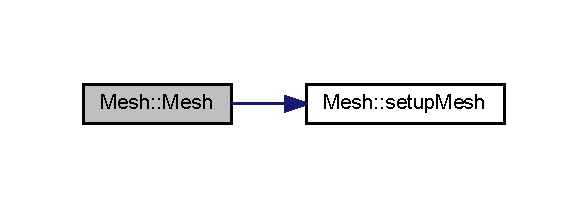
\includegraphics[width=282pt]{classMesh_af1baf95f510199fd2b3631e9daae79ce_cgraph}
\end{center}
\end{figure}


\subsection{Member Function Documentation}
\mbox{\Hypertarget{classMesh_a143c8d7c179801c6377853db26d4a19f}\label{classMesh_a143c8d7c179801c6377853db26d4a19f}} 
\index{Mesh@{Mesh}!Draw@{Draw}}
\index{Draw@{Draw}!Mesh@{Mesh}}
\subsubsection{\texorpdfstring{Draw()}{Draw()}}
{\footnotesize\ttfamily void Mesh\+::\+Draw (\begin{DoxyParamCaption}\item[{\mbox{\hyperlink{classShader}{Shader}}}]{shader }\end{DoxyParamCaption})}



Definition at line 50 of file Mesh.\+cpp.



References indices, and V\+AO.

\mbox{\Hypertarget{classMesh_aafa4e21067a9b0c4407daf5e3c9ea991}\label{classMesh_aafa4e21067a9b0c4407daf5e3c9ea991}} 
\index{Mesh@{Mesh}!setup\+Mesh@{setup\+Mesh}}
\index{setup\+Mesh@{setup\+Mesh}!Mesh@{Mesh}}
\subsubsection{\texorpdfstring{setup\+Mesh()}{setupMesh()}}
{\footnotesize\ttfamily void Mesh\+::setup\+Mesh (\begin{DoxyParamCaption}{ }\end{DoxyParamCaption})\hspace{0.3cm}{\ttfamily [private]}}



Definition at line 20 of file Mesh.\+cpp.



References E\+BO, indices, V\+AO, V\+BO, and vertices.



Referenced by Mesh().



\subsection{Member Data Documentation}
\mbox{\Hypertarget{classMesh_a894c6723c0172f4e38b2509582abfa6c}\label{classMesh_a894c6723c0172f4e38b2509582abfa6c}} 
\index{Mesh@{Mesh}!E\+BO@{E\+BO}}
\index{E\+BO@{E\+BO}!Mesh@{Mesh}}
\subsubsection{\texorpdfstring{E\+BO}{EBO}}
{\footnotesize\ttfamily G\+Luint Mesh\+::\+E\+BO\hspace{0.3cm}{\ttfamily [private]}}



Definition at line 44 of file Mesh.\+h.



Referenced by setup\+Mesh().

\mbox{\Hypertarget{classMesh_a5e55b84c6c967608bcf23ed7d68e4215}\label{classMesh_a5e55b84c6c967608bcf23ed7d68e4215}} 
\index{Mesh@{Mesh}!indices@{indices}}
\index{indices@{indices}!Mesh@{Mesh}}
\subsubsection{\texorpdfstring{indices}{indices}}
{\footnotesize\ttfamily std\+::vector$<$G\+Luint$>$ Mesh\+::indices}



Definition at line 37 of file Mesh.\+h.



Referenced by Draw(), Mesh(), and setup\+Mesh().

\mbox{\Hypertarget{classMesh_abf1e672703bf4f8e104f3b076faaf958}\label{classMesh_abf1e672703bf4f8e104f3b076faaf958}} 
\index{Mesh@{Mesh}!textures@{textures}}
\index{textures@{textures}!Mesh@{Mesh}}
\subsubsection{\texorpdfstring{textures}{textures}}
{\footnotesize\ttfamily std\+::vector$<$\mbox{\hyperlink{structTexture}{Texture}}$>$ Mesh\+::textures}



Definition at line 38 of file Mesh.\+h.



Referenced by Mesh().

\mbox{\Hypertarget{classMesh_a09b989b9d4df8ae595d7e80e091a4a5b}\label{classMesh_a09b989b9d4df8ae595d7e80e091a4a5b}} 
\index{Mesh@{Mesh}!V\+AO@{V\+AO}}
\index{V\+AO@{V\+AO}!Mesh@{Mesh}}
\subsubsection{\texorpdfstring{V\+AO}{VAO}}
{\footnotesize\ttfamily G\+Luint Mesh\+::\+V\+AO\hspace{0.3cm}{\ttfamily [private]}}



Definition at line 42 of file Mesh.\+h.



Referenced by Draw(), and setup\+Mesh().

\mbox{\Hypertarget{classMesh_a0d28b2c6fee628a13f43cae3f858569b}\label{classMesh_a0d28b2c6fee628a13f43cae3f858569b}} 
\index{Mesh@{Mesh}!V\+BO@{V\+BO}}
\index{V\+BO@{V\+BO}!Mesh@{Mesh}}
\subsubsection{\texorpdfstring{V\+BO}{VBO}}
{\footnotesize\ttfamily G\+Luint Mesh\+::\+V\+BO\hspace{0.3cm}{\ttfamily [private]}}



Definition at line 43 of file Mesh.\+h.



Referenced by setup\+Mesh().

\mbox{\Hypertarget{classMesh_a6465a888c97232a39e12aad008c969c3}\label{classMesh_a6465a888c97232a39e12aad008c969c3}} 
\index{Mesh@{Mesh}!vertices@{vertices}}
\index{vertices@{vertices}!Mesh@{Mesh}}
\subsubsection{\texorpdfstring{vertices}{vertices}}
{\footnotesize\ttfamily std\+::vector$<$\mbox{\hyperlink{structVertex}{Vertex}}$>$ Mesh\+::vertices}



Definition at line 36 of file Mesh.\+h.



Referenced by Mesh(), and setup\+Mesh().



The documentation for this class was generated from the following files\+:\begin{DoxyCompactItemize}
\item 
C\+:/\+Users/cfantacci/\+Git\+Hub/superimpose-\/mesh-\/lib/src/\+Superimpose\+Mesh/include/\+Superimpose\+Mesh/\mbox{\hyperlink{Mesh_8h}{Mesh.\+h}}\item 
C\+:/\+Users/cfantacci/\+Git\+Hub/superimpose-\/mesh-\/lib/src/\+Superimpose\+Mesh/src/\mbox{\hyperlink{Mesh_8cpp}{Mesh.\+cpp}}\end{DoxyCompactItemize}

\hypertarget{classModel}{}\section{Model Class Reference}
\label{classModel}\index{Model@{Model}}


{\ttfamily \#include $<$Model.\+h$>$}

\subsection*{Public Member Functions}
\begin{DoxyCompactItemize}
\item 
\mbox{\hyperlink{classModel_a97ced90b9b512521b2e5bdeaeac6b907}{Model}} (const G\+Lchar $\ast$path)
\item 
void \mbox{\hyperlink{classModel_a191a00d937b9e911bf4881ea14d79b6c}{Draw}} (\mbox{\hyperlink{classShader}{Shader}} shader)
\end{DoxyCompactItemize}
\subsection*{Private Member Functions}
\begin{DoxyCompactItemize}
\item 
void \mbox{\hyperlink{classModel_a3cd88224a93dc81a8503d42be807eb86}{load\+Model}} (std\+::string path)
\item 
void \mbox{\hyperlink{classModel_a23b167ce0d33f7e6ab5693cd5e81a9a5}{process\+Node}} (ai\+Node $\ast$node, const ai\+Scene $\ast$scene)
\item 
\mbox{\hyperlink{classMesh}{Mesh}} \mbox{\hyperlink{classModel_a95ae1a9980ded3d98b1c8785cb889d96}{process\+Mesh}} (ai\+Mesh $\ast$mesh, const ai\+Scene $\ast$scene)
\end{DoxyCompactItemize}
\subsection*{Private Attributes}
\begin{DoxyCompactItemize}
\item 
std\+::vector$<$ \mbox{\hyperlink{classMesh}{Mesh}} $>$ \mbox{\hyperlink{classModel_a538e42901dcfba59471072a48a162163}{meshes}}
\item 
std\+::string \mbox{\hyperlink{classModel_a5ea3aa111c7a7d179e93dcc0bb567701}{directory}}
\item 
std\+::vector$<$ \mbox{\hyperlink{structTexture}{Texture}} $>$ \mbox{\hyperlink{classModel_a866353fd9967b57286864fac87799ae1}{textures\+\_\+loaded}}
\end{DoxyCompactItemize}


\subsection{Detailed Description}


Definition at line 14 of file Model.\+h.



\subsection{Constructor \& Destructor Documentation}
\mbox{\Hypertarget{classModel_a97ced90b9b512521b2e5bdeaeac6b907}\label{classModel_a97ced90b9b512521b2e5bdeaeac6b907}} 
\index{Model@{Model}!Model@{Model}}
\index{Model@{Model}!Model@{Model}}
\subsubsection{\texorpdfstring{Model()}{Model()}}
{\footnotesize\ttfamily Model\+::\+Model (\begin{DoxyParamCaption}\item[{const G\+Lchar $\ast$}]{path }\end{DoxyParamCaption})}



Definition at line 11 of file Model.\+cpp.



References load\+Model().

Here is the call graph for this function\+:
\nopagebreak
\begin{figure}[H]
\begin{center}
\leavevmode
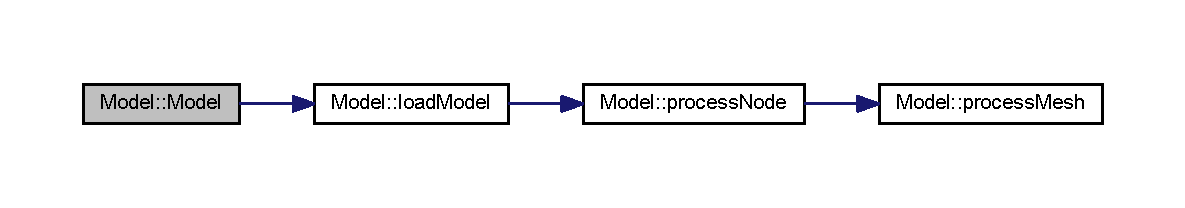
\includegraphics[width=350pt]{classModel_a97ced90b9b512521b2e5bdeaeac6b907_cgraph}
\end{center}
\end{figure}


\subsection{Member Function Documentation}
\mbox{\Hypertarget{classModel_a191a00d937b9e911bf4881ea14d79b6c}\label{classModel_a191a00d937b9e911bf4881ea14d79b6c}} 
\index{Model@{Model}!Draw@{Draw}}
\index{Draw@{Draw}!Model@{Model}}
\subsubsection{\texorpdfstring{Draw()}{Draw()}}
{\footnotesize\ttfamily void Model\+::\+Draw (\begin{DoxyParamCaption}\item[{\mbox{\hyperlink{classShader}{Shader}}}]{shader }\end{DoxyParamCaption})}



Definition at line 17 of file Model.\+cpp.



References meshes.

\mbox{\Hypertarget{classModel_a3cd88224a93dc81a8503d42be807eb86}\label{classModel_a3cd88224a93dc81a8503d42be807eb86}} 
\index{Model@{Model}!load\+Model@{load\+Model}}
\index{load\+Model@{load\+Model}!Model@{Model}}
\subsubsection{\texorpdfstring{load\+Model()}{loadModel()}}
{\footnotesize\ttfamily void Model\+::load\+Model (\begin{DoxyParamCaption}\item[{std\+::string}]{path }\end{DoxyParamCaption})\hspace{0.3cm}{\ttfamily [private]}}



Definition at line 26 of file Model.\+cpp.



References directory, and process\+Node().



Referenced by Model().

Here is the call graph for this function\+:
\nopagebreak
\begin{figure}[H]
\begin{center}
\leavevmode
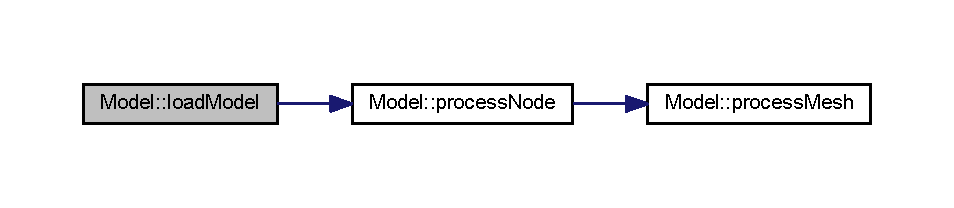
\includegraphics[width=350pt]{classModel_a3cd88224a93dc81a8503d42be807eb86_cgraph}
\end{center}
\end{figure}
\mbox{\Hypertarget{classModel_a95ae1a9980ded3d98b1c8785cb889d96}\label{classModel_a95ae1a9980ded3d98b1c8785cb889d96}} 
\index{Model@{Model}!process\+Mesh@{process\+Mesh}}
\index{process\+Mesh@{process\+Mesh}!Model@{Model}}
\subsubsection{\texorpdfstring{process\+Mesh()}{processMesh()}}
{\footnotesize\ttfamily \mbox{\hyperlink{classMesh}{Mesh}} Model\+::process\+Mesh (\begin{DoxyParamCaption}\item[{ai\+Mesh $\ast$}]{mesh,  }\item[{const ai\+Scene $\ast$}]{scene }\end{DoxyParamCaption})\hspace{0.3cm}{\ttfamily [private]}}



Definition at line 68 of file Model.\+cpp.



References Vertex\+::\+Normal, Vertex\+::\+Position, and Vertex\+::\+Tex\+Coords.



Referenced by process\+Node().

\mbox{\Hypertarget{classModel_a23b167ce0d33f7e6ab5693cd5e81a9a5}\label{classModel_a23b167ce0d33f7e6ab5693cd5e81a9a5}} 
\index{Model@{Model}!process\+Node@{process\+Node}}
\index{process\+Node@{process\+Node}!Model@{Model}}
\subsubsection{\texorpdfstring{process\+Node()}{processNode()}}
{\footnotesize\ttfamily void Model\+::process\+Node (\begin{DoxyParamCaption}\item[{ai\+Node $\ast$}]{node,  }\item[{const ai\+Scene $\ast$}]{scene }\end{DoxyParamCaption})\hspace{0.3cm}{\ttfamily [private]}}



Definition at line 51 of file Model.\+cpp.



References meshes, and process\+Mesh().



Referenced by load\+Model().

Here is the call graph for this function\+:
\nopagebreak
\begin{figure}[H]
\begin{center}
\leavevmode
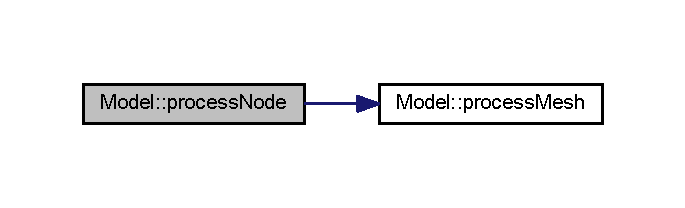
\includegraphics[width=329pt]{classModel_a23b167ce0d33f7e6ab5693cd5e81a9a5_cgraph}
\end{center}
\end{figure}


\subsection{Member Data Documentation}
\mbox{\Hypertarget{classModel_a5ea3aa111c7a7d179e93dcc0bb567701}\label{classModel_a5ea3aa111c7a7d179e93dcc0bb567701}} 
\index{Model@{Model}!directory@{directory}}
\index{directory@{directory}!Model@{Model}}
\subsubsection{\texorpdfstring{directory}{directory}}
{\footnotesize\ttfamily std\+::string Model\+::directory\hspace{0.3cm}{\ttfamily [private]}}



Definition at line 25 of file Model.\+h.



Referenced by load\+Model().

\mbox{\Hypertarget{classModel_a538e42901dcfba59471072a48a162163}\label{classModel_a538e42901dcfba59471072a48a162163}} 
\index{Model@{Model}!meshes@{meshes}}
\index{meshes@{meshes}!Model@{Model}}
\subsubsection{\texorpdfstring{meshes}{meshes}}
{\footnotesize\ttfamily std\+::vector$<$\mbox{\hyperlink{classMesh}{Mesh}}$>$ Model\+::meshes\hspace{0.3cm}{\ttfamily [private]}}



Definition at line 24 of file Model.\+h.



Referenced by Draw(), and process\+Node().

\mbox{\Hypertarget{classModel_a866353fd9967b57286864fac87799ae1}\label{classModel_a866353fd9967b57286864fac87799ae1}} 
\index{Model@{Model}!textures\+\_\+loaded@{textures\+\_\+loaded}}
\index{textures\+\_\+loaded@{textures\+\_\+loaded}!Model@{Model}}
\subsubsection{\texorpdfstring{textures\+\_\+loaded}{textures\_loaded}}
{\footnotesize\ttfamily std\+::vector$<$\mbox{\hyperlink{structTexture}{Texture}}$>$ Model\+::textures\+\_\+loaded\hspace{0.3cm}{\ttfamily [private]}}



Definition at line 26 of file Model.\+h.



The documentation for this class was generated from the following files\+:\begin{DoxyCompactItemize}
\item 
C\+:/\+Users/cfantacci/\+Git\+Hub/superimpose-\/mesh-\/lib/src/\+Superimpose\+Mesh/include/\+Superimpose\+Mesh/\mbox{\hyperlink{Model_8h}{Model.\+h}}\item 
C\+:/\+Users/cfantacci/\+Git\+Hub/superimpose-\/mesh-\/lib/src/\+Superimpose\+Mesh/src/\mbox{\hyperlink{Model_8cpp}{Model.\+cpp}}\end{DoxyCompactItemize}

\hypertarget{classShader}{}\section{Shader Class Reference}
\label{classShader}\index{Shader@{Shader}}


{\ttfamily \#include $<$Shader.\+h$>$}

\subsection*{Public Member Functions}
\begin{DoxyCompactItemize}
\item 
\mbox{\hyperlink{classShader_a03421a8419cdad4b84cf58ecdb156879}{Shader}} (const G\+Lchar $\ast$vertex\+Path, const G\+Lchar $\ast$fragment\+Path)
\item 
void \mbox{\hyperlink{classShader_a8e53260be208ebf6c804a0d309e74097}{install}} ()
\item 
void \mbox{\hyperlink{classShader_afa6fb33b37c9385cf62a836092da570b}{uninstall}} ()
\end{DoxyCompactItemize}
\subsection*{Public Attributes}
\begin{DoxyCompactItemize}
\item 
G\+Luint \mbox{\hyperlink{classShader_a51b23253846bc84dcc2ef06612679012}{Program}}
\end{DoxyCompactItemize}


\subsection{Detailed Description}


Definition at line 9 of file Shader.\+h.



\subsection{Constructor \& Destructor Documentation}
\mbox{\Hypertarget{classShader_a03421a8419cdad4b84cf58ecdb156879}\label{classShader_a03421a8419cdad4b84cf58ecdb156879}} 
\index{Shader@{Shader}!Shader@{Shader}}
\index{Shader@{Shader}!Shader@{Shader}}
\subsubsection{\texorpdfstring{Shader()}{Shader()}}
{\footnotesize\ttfamily Shader\+::\+Shader (\begin{DoxyParamCaption}\item[{const G\+Lchar $\ast$}]{vertex\+Path,  }\item[{const G\+Lchar $\ast$}]{fragment\+Path }\end{DoxyParamCaption})}



Definition at line 9 of file Shader.\+cpp.



References Program.



\subsection{Member Function Documentation}
\mbox{\Hypertarget{classShader_a8e53260be208ebf6c804a0d309e74097}\label{classShader_a8e53260be208ebf6c804a0d309e74097}} 
\index{Shader@{Shader}!install@{install}}
\index{install@{install}!Shader@{Shader}}
\subsubsection{\texorpdfstring{install()}{install()}}
{\footnotesize\ttfamily void Shader\+::install (\begin{DoxyParamCaption}{ }\end{DoxyParamCaption})}



Definition at line 98 of file Shader.\+cpp.



References Program.



Referenced by S\+I\+C\+A\+D\+::set\+Background(), S\+I\+C\+A\+D\+::set\+Projection\+Matrix(), and S\+I\+C\+A\+D\+::superimpose().

\mbox{\Hypertarget{classShader_afa6fb33b37c9385cf62a836092da570b}\label{classShader_afa6fb33b37c9385cf62a836092da570b}} 
\index{Shader@{Shader}!uninstall@{uninstall}}
\index{uninstall@{uninstall}!Shader@{Shader}}
\subsubsection{\texorpdfstring{uninstall()}{uninstall()}}
{\footnotesize\ttfamily void Shader\+::uninstall (\begin{DoxyParamCaption}{ }\end{DoxyParamCaption})}



Definition at line 104 of file Shader.\+cpp.



Referenced by S\+I\+C\+A\+D\+::set\+Background(), S\+I\+C\+A\+D\+::set\+Projection\+Matrix(), and S\+I\+C\+A\+D\+::superimpose().



\subsection{Member Data Documentation}
\mbox{\Hypertarget{classShader_a51b23253846bc84dcc2ef06612679012}\label{classShader_a51b23253846bc84dcc2ef06612679012}} 
\index{Shader@{Shader}!Program@{Program}}
\index{Program@{Program}!Shader@{Shader}}
\subsubsection{\texorpdfstring{Program}{Program}}
{\footnotesize\ttfamily G\+Luint Shader\+::\+Program}



Definition at line 22 of file Shader.\+h.



Referenced by install(), S\+I\+C\+A\+D\+::set\+Background(), S\+I\+C\+A\+D\+::set\+Projection\+Matrix(), Shader(), and S\+I\+C\+A\+D\+::superimpose().



The documentation for this class was generated from the following files\+:\begin{DoxyCompactItemize}
\item 
C\+:/\+Users/cfantacci/\+Git\+Hub/superimpose-\/mesh-\/lib/src/\+Superimpose\+Mesh/include/\+Superimpose\+Mesh/\mbox{\hyperlink{Shader_8h}{Shader.\+h}}\item 
C\+:/\+Users/cfantacci/\+Git\+Hub/superimpose-\/mesh-\/lib/src/\+Superimpose\+Mesh/src/\mbox{\hyperlink{Shader_8cpp}{Shader.\+cpp}}\end{DoxyCompactItemize}

\hypertarget{classSICAD}{}\section{S\+I\+C\+AD Class Reference}
\label{classSICAD}\index{S\+I\+C\+AD@{S\+I\+C\+AD}}


A \mbox{\hyperlink{classSuperimpose}{Superimpose}} derived class to superimpose mesh models on top of images.  




{\ttfamily \#include $<$S\+I\+C\+A\+D.\+h$>$}



Inheritance diagram for S\+I\+C\+AD\+:
\nopagebreak
\begin{figure}[H]
\begin{center}
\leavevmode
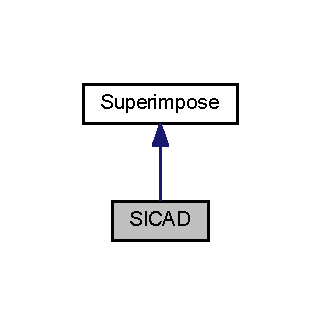
\includegraphics[width=154pt]{classSICAD__inherit__graph}
\end{center}
\end{figure}
\subsection*{Public Types}
\begin{DoxyCompactItemize}
\item 
enum \mbox{\hyperlink{classSICAD_a7e092dede6f660355462d6d548214198}{M\+I\+P\+Maps}} \{ \mbox{\hyperlink{classSICAD_a7e092dede6f660355462d6d548214198ad879c351426770bc0b13c3628db1e636}{M\+I\+P\+Maps\+::nearest}}, 
\mbox{\hyperlink{classSICAD_a7e092dede6f660355462d6d548214198a9a932b3cb396238423eb2f33ec17d6aa}{M\+I\+P\+Maps\+::linear}}
 \}
\item 
typedef std\+::unordered\+\_\+map$<$ std\+::string, std\+::string $>$ \mbox{\hyperlink{classSICAD_a9e1e1460d4c0f331b4fd015aae4dd721}{Model\+Path\+Container}}
\item 
typedef std\+::pair$<$ std\+::string, std\+::string $>$ \mbox{\hyperlink{classSICAD_a5148c8a96c82625706ce2e5b86b52dd7}{Model\+Path\+Element}}
\item 
typedef std\+::unordered\+\_\+map$<$ std\+::string, \mbox{\hyperlink{classModel}{Model}} $\ast$ $>$ \mbox{\hyperlink{classSICAD_aca3c9693d298f2e8dc171194c6a7507c}{Model\+Container}}
\item 
typedef std\+::pair$<$ std\+::string, \mbox{\hyperlink{classModel}{Model}} $\ast$ $>$ \mbox{\hyperlink{classSICAD_af999665097d7cdf11780735bf24a6956}{Model\+Element}}
\item 
typedef std\+::vector$<$ double $>$ \mbox{\hyperlink{classSuperimpose_a85d40a5caf19f486d1e0c15c0a025378}{Model\+Pose}}
\item 
typedef std\+::multimap$<$ std\+::string, \mbox{\hyperlink{classSuperimpose_a85d40a5caf19f486d1e0c15c0a025378}{Model\+Pose}} $>$ \mbox{\hyperlink{classSuperimpose_a178e3d4e2def6635bfcf9454dd4b5d22}{Model\+Pose\+Container}}
\item 
typedef std\+::pair$<$ std\+::string, \mbox{\hyperlink{classSuperimpose_a85d40a5caf19f486d1e0c15c0a025378}{Model\+Pose}} $>$ \mbox{\hyperlink{classSuperimpose_a1e02e0225687b42296dcfee4eadf8a55}{Model\+Pose\+Container\+Element}}
\end{DoxyCompactItemize}
\subsection*{Public Member Functions}
\begin{DoxyCompactItemize}
\item 
\mbox{\hyperlink{classSICAD_a6fe9d4a644f468438264842896684a2c}{S\+I\+C\+AD}} ()
\item 
\mbox{\hyperlink{classSICAD_af6f17b4221b2d2725de7663c1a990175}{S\+I\+C\+AD}} (const \mbox{\hyperlink{classSICAD_a9e1e1460d4c0f331b4fd015aae4dd721}{Model\+Path\+Container}} \&objfile\+\_\+map, const bool window\+\_\+visible)
\item 
\mbox{\hyperlink{classSICAD_aa3cd941a7aa5f6620c6591c3b21a081c}{S\+I\+C\+AD}} (const \mbox{\hyperlink{classSICAD_a9e1e1460d4c0f331b4fd015aae4dd721}{Model\+Path\+Container}} \&objfile\+\_\+map, const std\+::string \&shader\+\_\+folder, const bool window\+\_\+visible)
\item 
\mbox{\hyperlink{classSICAD_a2f0ac6e07e5b0cf7e8a99205bf4bc447}{S\+I\+C\+AD}} (const \mbox{\hyperlink{classSICAD_a9e1e1460d4c0f331b4fd015aae4dd721}{Model\+Path\+Container}} \&objfile\+\_\+map, const G\+Lsizei cam\+\_\+width, const G\+Lsizei cam\+\_\+height, const std\+::string \&shader\+\_\+folder, const bool window\+\_\+visible)
\item 
\mbox{\hyperlink{classSICAD_abebce8e8feb344ad23caed3e2a8b732a}{S\+I\+C\+AD}} (const \mbox{\hyperlink{classSICAD_a9e1e1460d4c0f331b4fd015aae4dd721}{Model\+Path\+Container}} \&objfile\+\_\+map, const G\+Lsizei cam\+\_\+width, const G\+Lsizei cam\+\_\+height, const G\+Lint num\+\_\+images, const std\+::string \&shader\+\_\+folder, const bool window\+\_\+visible)
\item 
\mbox{\hyperlink{classSICAD_abcb9bb154f73472447affb9bb16dcec7}{S\+I\+C\+AD}} (const \mbox{\hyperlink{classSICAD_a9e1e1460d4c0f331b4fd015aae4dd721}{Model\+Path\+Container}} \&objfile\+\_\+map, const G\+Lsizei cam\+\_\+width, const G\+Lsizei cam\+\_\+height, const G\+Lint num\+\_\+images, const std\+::vector$<$ float $>$ \&ogl\+\_\+to\+\_\+cam, const std\+::string \&shader\+\_\+folder, const bool window\+\_\+visible)
\item 
\mbox{\hyperlink{classSICAD_a6ddc65ccbfea740515782c4b0dc25a0c}{S\+I\+C\+AD}} (const \mbox{\hyperlink{classSICAD_a9e1e1460d4c0f331b4fd015aae4dd721}{Model\+Path\+Container}} \&objfile\+\_\+map, const G\+Lsizei cam\+\_\+width, const G\+Lsizei cam\+\_\+height, const G\+Lfloat cam\+\_\+fx, const G\+Lfloat cam\+\_\+fy, const G\+Lfloat cam\+\_\+cx, const G\+Lfloat cam\+\_\+cy, const std\+::string \&shader\+\_\+folder, const bool window\+\_\+visible)
\item 
\mbox{\hyperlink{classSICAD_a1d217cbdc1670f8c5885c413e4acbede}{S\+I\+C\+AD}} (const \mbox{\hyperlink{classSICAD_a9e1e1460d4c0f331b4fd015aae4dd721}{Model\+Path\+Container}} \&objfile\+\_\+map, const G\+Lsizei cam\+\_\+width, const G\+Lsizei cam\+\_\+height, const G\+Lfloat cam\+\_\+fx, const G\+Lfloat cam\+\_\+fy, const G\+Lfloat cam\+\_\+cx, const G\+Lfloat cam\+\_\+cy, const G\+Lint num\+\_\+images, const std\+::string \&shader\+\_\+folder, const bool window\+\_\+visible)
\item 
\mbox{\hyperlink{classSICAD_ac4e6349b361e3ec41d828e0d0f77f12b}{S\+I\+C\+AD}} (const \mbox{\hyperlink{classSICAD_a9e1e1460d4c0f331b4fd015aae4dd721}{Model\+Path\+Container}} \&objfile\+\_\+map, const G\+Lsizei cam\+\_\+width, const G\+Lsizei cam\+\_\+height, const G\+Lfloat cam\+\_\+fx, const G\+Lfloat cam\+\_\+fy, const G\+Lfloat cam\+\_\+cx, const G\+Lfloat cam\+\_\+cy, const G\+Lint num\+\_\+images, const std\+::vector$<$ float $>$ \&ogl\+\_\+to\+\_\+cam, const std\+::string \&shader\+\_\+folder, const bool window\+\_\+visible)
\begin{DoxyCompactList}\small\item\em Create a \mbox{\hyperlink{classSICAD}{S\+I\+C\+AD}} object with a dedicated Open\+GL window and context. \end{DoxyCompactList}\item 
bool \mbox{\hyperlink{classSICAD_a04e1291dc1a51b2dee87dbe9a5b3a316}{init\+S\+I\+C\+AD}} (const \mbox{\hyperlink{classSICAD_a9e1e1460d4c0f331b4fd015aae4dd721}{Model\+Path\+Container}} \&objfile\+\_\+map, const G\+Lsizei cam\+\_\+width, const G\+Lsizei cam\+\_\+height, const G\+Lint num\+\_\+images, const std\+::vector$<$ float $>$ \&ogl\+\_\+to\+\_\+cam, const std\+::string \&shader\+\_\+folder, const bool window\+\_\+visible)
\item 
bool \mbox{\hyperlink{classSICAD_abb2b0250a885435828d5255645e06ac8}{init\+S\+I\+C\+AD}} (const \mbox{\hyperlink{classSICAD_a9e1e1460d4c0f331b4fd015aae4dd721}{Model\+Path\+Container}} \&objfile\+\_\+map, const G\+Lsizei cam\+\_\+width, const G\+Lsizei cam\+\_\+height, const G\+Lfloat cam\+\_\+fx, const G\+Lfloat cam\+\_\+fy, const G\+Lfloat cam\+\_\+cx, const G\+Lfloat cam\+\_\+cy, const G\+Lint num\+\_\+images, const std\+::vector$<$ float $>$ \&ogl\+\_\+to\+\_\+cam, const std\+::string \&shader\+\_\+folder, const bool window\+\_\+visible)
\item 
virtual \mbox{\hyperlink{classSICAD_a4e3d6d1f90ea2261dcd8507ee8709360}{$\sim$\+S\+I\+C\+AD}} ()
\item 
bool \mbox{\hyperlink{classSICAD_aaf003ab2ac8bc5ebdef6611ca1547e73}{get\+Ogl\+Window\+Should\+Close}} ()
\item 
void \mbox{\hyperlink{classSICAD_a0e42acab32252ddc878794f365ee1037}{set\+Ogl\+Window\+Should\+Close}} (bool should\+\_\+close)
\item 
bool \mbox{\hyperlink{classSICAD_a356e0ac8a0f130952a72326bedd4ab60}{superimpose}} (const \mbox{\hyperlink{classSuperimpose_a178e3d4e2def6635bfcf9454dd4b5d22}{Model\+Pose\+Container}} \&objpos\+\_\+map, const double $\ast$cam\+\_\+x, const double $\ast$cam\+\_\+o, cv\+::\+Mat \&img) override
\begin{DoxyCompactList}\small\item\em \mbox{\hyperlink{classSuperimpose}{Superimpose}} one of the mesh models loaded during \mbox{\hyperlink{classSICAD}{S\+I\+C\+AD}} object construction in a given pose from a particular camera viewpoint. \end{DoxyCompactList}\item 
virtual bool \mbox{\hyperlink{classSICAD_ab15f84cec5a65c8dd6cad85f9b0e1993}{superimpose}} (const std\+::vector$<$ \mbox{\hyperlink{classSuperimpose_a178e3d4e2def6635bfcf9454dd4b5d22}{Model\+Pose\+Container}} $>$ \&objpos\+\_\+multimap, const double $\ast$cam\+\_\+x, const double $\ast$cam\+\_\+o, cv\+::\+Mat \&img)
\item 
virtual bool \mbox{\hyperlink{classSICAD_af6c19a679de29992c5f9609f4424add0}{superimpose}} (const \mbox{\hyperlink{classSuperimpose_a178e3d4e2def6635bfcf9454dd4b5d22}{Model\+Pose\+Container}} \&objpos\+\_\+map, const double $\ast$cam\+\_\+x, const double $\ast$cam\+\_\+o, cv\+::\+Mat \&img, const G\+Lsizei cam\+\_\+width, const G\+Lsizei cam\+\_\+height, const G\+Lfloat cam\+\_\+fx, const G\+Lfloat cam\+\_\+fy, const G\+Lfloat cam\+\_\+cx, const G\+Lfloat cam\+\_\+cy)
\item 
virtual bool \mbox{\hyperlink{classSICAD_a269e238387393b44177daa4eae88fedd}{superimpose}} (const std\+::vector$<$ \mbox{\hyperlink{classSuperimpose_a178e3d4e2def6635bfcf9454dd4b5d22}{Model\+Pose\+Container}} $>$ \&objpos\+\_\+multimap, const double $\ast$cam\+\_\+x, const double $\ast$cam\+\_\+o, cv\+::\+Mat \&img, const G\+Lsizei cam\+\_\+width, const G\+Lsizei cam\+\_\+height, const G\+Lfloat cam\+\_\+fx, const G\+Lfloat cam\+\_\+fy, const G\+Lfloat cam\+\_\+cx, const G\+Lfloat cam\+\_\+cy)
\item 
bool \mbox{\hyperlink{classSICAD_a39cdff6871d32429d8ba95b776e0b874}{set\+Projection\+Matrix}} (const G\+Lsizei cam\+\_\+width, const G\+Lsizei cam\+\_\+height, const G\+Lfloat cam\+\_\+fx, const G\+Lfloat cam\+\_\+fy, const G\+Lfloat cam\+\_\+cx, const G\+Lfloat cam\+\_\+cy)
\item 
bool \mbox{\hyperlink{classSICAD_a170bd325654aed9eb81062ac610608fa}{get\+Background\+Opt}} () const
\item 
void \mbox{\hyperlink{classSICAD_a07921943ad3d4016dcbe76135e799754}{set\+Background\+Opt}} (bool show\+\_\+background)
\item 
G\+Lenum \mbox{\hyperlink{classSICAD_af65b5ad73e2c0e872face157b56bd68b}{get\+Wireframe\+Opt}} () const
\item 
void \mbox{\hyperlink{classSICAD_a4cf80a273b6b0d946cd298472c63ddd4}{set\+Wireframe\+Opt}} (bool show\+\_\+mesh\+\_\+wires)
\item 
\mbox{\hyperlink{classSICAD_a7e092dede6f660355462d6d548214198}{M\+I\+P\+Maps}} \mbox{\hyperlink{classSICAD_a8033a99745f595ea5205e3830cabc389}{get\+Mipmaps\+Opt}} () const
\item 
int \mbox{\hyperlink{classSICAD_a728f82ebbfeea54f3fef2fc0c56a4964}{get\+Tiles\+Number}} () const
\item 
int \mbox{\hyperlink{classSICAD_a9e3dd48dfd83ea0bd00d64dacc4fbd40}{get\+Tiles\+Rows}} () const
\item 
int \mbox{\hyperlink{classSICAD_a2ba3a0aeb3dab9996bdeed19a16eae56}{get\+Tiles\+Cols}} () const
\end{DoxyCompactItemize}
\subsection*{Private Member Functions}
\begin{DoxyCompactItemize}
\item 
bool \mbox{\hyperlink{classSICAD_a102619690ab32e300405d22d52e36a5e}{init\+O\+GL}} (const G\+Lsizei width, const G\+Lsizei height, const G\+Lint num\+\_\+viewports, const bool window\+\_\+visibile)
\item 
glm\+::mat4 \mbox{\hyperlink{classSICAD_a1bdece095865249df4cb4e6a7ad2901e}{get\+View\+Transformation\+Matrix}} (const double $\ast$cam\+\_\+x, const double $\ast$cam\+\_\+o)
\item 
void \mbox{\hyperlink{classSICAD_a8238a2b2c488c8b7ba85d5b2a0bf00ac}{poll\+Or\+Post\+Event}} ()
\item 
void \mbox{\hyperlink{classSICAD_a25b180f54f2e93d69b291cc225600c8e}{set\+Background}} (cv\+::\+Mat \&img)
\item 
void \mbox{\hyperlink{classSICAD_ae7af7aba5d81b9f1cc3e273a55811a70}{set\+Wireframe}} (G\+Lenum mode)
\item 
void \mbox{\hyperlink{classSICAD_a2603ec5cb9a31bc7be0a335ef513ab0d}{factorize\+\_\+int}} (const G\+Lsizei area, const G\+Lsizei width\+\_\+limit, const G\+Lsizei height\+\_\+limit, G\+Lsizei \&width, G\+Lsizei \&height)
\end{DoxyCompactItemize}
\subsection*{Static Private Member Functions}
\begin{DoxyCompactItemize}
\item 
static void \mbox{\hyperlink{classSICAD_ae2d8d44b5bbcf7329e180aafda2df386}{callback\+Keypress}} (G\+L\+F\+Wwindow $\ast$window, int key, int scancode, int action, int mode)
\end{DoxyCompactItemize}
\subsection*{Private Attributes}
\begin{DoxyCompactItemize}
\item 
bool \mbox{\hyperlink{classSICAD_aa624c978497506de4a255c5f0301579f}{is\+\_\+initialized\+\_\+}} = false
\item 
bool \mbox{\hyperlink{classSICAD_a0eb57d114f3f6b50be13bd882552b2f7}{has\+\_\+proj\+\_\+matrix\+\_\+}} = false
\item 
const std\+::string \mbox{\hyperlink{classSICAD_a9eb34b659cac13b8442ca821455cc1f1}{log\+\_\+\+I\+D\+\_\+}} = \char`\"{}\mbox{[}SI-\/C\+AD\mbox{]}\char`\"{}
\item 
G\+L\+F\+Wwindow $\ast$ \mbox{\hyperlink{classSICAD_a3e55fa9ffa99ef200bfc15d6a105698a}{window\+\_\+}} = nullptr
\item 
G\+Lint \mbox{\hyperlink{classSICAD_a68723ee57cc9a1e02bc0dbda54a584ff}{tiles\+\_\+num\+\_\+}} = 0
\item 
G\+Lsizei \mbox{\hyperlink{classSICAD_ac2678cc1ad1b008912fec7e6892b23e1}{tiles\+\_\+cols\+\_\+}} = 0
\item 
G\+Lsizei \mbox{\hyperlink{classSICAD_aca3efa8f3fb75b3ee02474d4ec00e49e}{tiles\+\_\+rows\+\_\+}} = 0
\item 
G\+Lsizei \mbox{\hyperlink{classSICAD_ade37d5c3960d164acaa749745f55070f}{image\+\_\+width\+\_\+}} = 0
\item 
G\+Lsizei \mbox{\hyperlink{classSICAD_a093da94bc84a46d08f71051c4d88c176}{image\+\_\+height\+\_\+}} = 0
\item 
glm\+::mat3 \mbox{\hyperlink{classSICAD_a95af2758122e6420369516fd13fd03cc}{ogl\+\_\+to\+\_\+cam\+\_\+}} = glm\+::mat3(1.\+0f)
\item 
G\+Lsizei \mbox{\hyperlink{classSICAD_a08c86b826a1784b132bac3f0792fc604}{framebuffer\+\_\+width\+\_\+}} = 0
\item 
G\+Lsizei \mbox{\hyperlink{classSICAD_a3361bb03e52bc0554bb1e3670ef3a0f9}{framebuffer\+\_\+height\+\_\+}} = 0
\item 
G\+Lsizei \mbox{\hyperlink{classSICAD_acbd2113a0cc446db6f59fdedd890aad9}{render\+\_\+img\+\_\+width\+\_\+}} = 0
\item 
G\+Lsizei \mbox{\hyperlink{classSICAD_a29691bc258b500253364c9688f7af655}{render\+\_\+img\+\_\+height\+\_\+}} = 0
\item 
const G\+Lfloat \mbox{\hyperlink{classSICAD_a690437655965101bad97d32e98015dd5}{near\+\_\+}} = 0.\+001f
\item 
const G\+Lfloat \mbox{\hyperlink{classSICAD_a4c4d2e249ac824528e1fe9f97fa207d9}{far\+\_\+}} = 1000.\+0f
\item 
std\+::thread\+::id \mbox{\hyperlink{classSICAD_a6a4623d27b2ee48ad0db90bd075c708c}{main\+\_\+thread\+\_\+id\+\_\+}}
\item 
bool \mbox{\hyperlink{classSICAD_a8db9e37d71a14883be4879e9ea4b6a02}{show\+\_\+background\+\_\+}} = false
\item 
G\+Lenum \mbox{\hyperlink{classSICAD_a9c4c3ba5d071f763ee1956fa31faa3f8}{show\+\_\+mesh\+\_\+mode\+\_\+}} = G\+L\+\_\+\+F\+I\+LL
\item 
\mbox{\hyperlink{classSICAD_a7e092dede6f660355462d6d548214198}{M\+I\+P\+Maps}} \mbox{\hyperlink{classSICAD_a34b0de96321855145937cc5858c019b0}{mesh\+\_\+mmaps\+\_\+}} = \mbox{\hyperlink{classSICAD_a7e092dede6f660355462d6d548214198ad879c351426770bc0b13c3628db1e636}{M\+I\+P\+Maps\+::nearest}}
\item 
\mbox{\hyperlink{classShader}{Shader}} $\ast$ \mbox{\hyperlink{classSICAD_a46edf33acc9f7ea3bd98c7ee6388ce9c}{shader\+\_\+background\+\_\+}} = nullptr
\item 
\mbox{\hyperlink{classShader}{Shader}} $\ast$ \mbox{\hyperlink{classSICAD_a6c11f0e8dc8cbdd91748c230fc680833}{shader\+\_\+cad\+\_\+}} = nullptr
\item 
\mbox{\hyperlink{classShader}{Shader}} $\ast$ \mbox{\hyperlink{classSICAD_ac921e60623f3797253bcbcdd445b903b}{shader\+\_\+frame\+\_\+}} = nullptr
\item 
\mbox{\hyperlink{classSICAD_aca3c9693d298f2e8dc171194c6a7507c}{Model\+Container}} \mbox{\hyperlink{classSICAD_a05fea2b5b027a3b7f37ef9ea4ecd64f0}{model\+\_\+obj\+\_\+}}
\item 
G\+Luint \mbox{\hyperlink{classSICAD_a2c173ad18d42e090b46a539f92f3fe9d}{fbo\+\_\+}}
\item 
G\+Luint \mbox{\hyperlink{classSICAD_a50f1ec3b2545ca40d58466735da80fc6}{texture\+\_\+color\+\_\+buffer\+\_\+}}
\item 
G\+Luint \mbox{\hyperlink{classSICAD_a2fed5ac56bb2206fe8f6eccc9d784015}{texture\+\_\+depth\+\_\+buffer\+\_\+}}
\item 
G\+Luint \mbox{\hyperlink{classSICAD_a2728fb0fa0be11f0992bc81b4873da4f}{texture\+\_\+background\+\_\+}}
\item 
G\+Luint \mbox{\hyperlink{classSICAD_a19306fe768bae547e18a3b9366e37389}{vao\+\_\+background\+\_\+}}
\item 
G\+Luint \mbox{\hyperlink{classSICAD_a2cdcd11dd55a4b02b85d7c32435cc719}{ebo\+\_\+background\+\_\+}}
\item 
G\+Luint \mbox{\hyperlink{classSICAD_a86d6184b8c557460317a158e8d9508d1}{vbo\+\_\+background\+\_\+}}
\item 
G\+Luint \mbox{\hyperlink{classSICAD_ae91abeb0fe30f27e0fc40649235f3437}{vao\+\_\+frame\+\_\+}}
\item 
G\+Luint \mbox{\hyperlink{classSICAD_af58ffe3edf622ab96f669fcd6e210be9}{vbo\+\_\+frame\+\_\+}}
\item 
glm\+::mat4 \mbox{\hyperlink{classSICAD_ad5945f84df0d90113a24b2001ecbc832}{back\+\_\+proj\+\_\+}}
\item 
glm\+::mat4 \mbox{\hyperlink{classSICAD_afb91b682fd1f6629f163ab321869e7e0}{projection\+\_\+}}
\end{DoxyCompactItemize}
\subsection*{Static Private Attributes}
\begin{DoxyCompactItemize}
\item 
static int \mbox{\hyperlink{classSICAD_a16f7c3c77ddea5ba57bbcbcdd7a8d125}{class\+\_\+counter\+\_\+}} = 0
\item 
static G\+Lsizei \mbox{\hyperlink{classSICAD_aca24504d58ce97106dbc95925f36fca0}{renderbuffer\+\_\+size\+\_\+}} = 0
\end{DoxyCompactItemize}


\subsection{Detailed Description}
A \mbox{\hyperlink{classSuperimpose}{Superimpose}} derived class to superimpose mesh models on top of images. 

Definition at line 21 of file S\+I\+C\+A\+D.\+h.



\subsection{Member Typedef Documentation}
\mbox{\Hypertarget{classSICAD_aca3c9693d298f2e8dc171194c6a7507c}\label{classSICAD_aca3c9693d298f2e8dc171194c6a7507c}} 
\index{S\+I\+C\+AD@{S\+I\+C\+AD}!Model\+Container@{Model\+Container}}
\index{Model\+Container@{Model\+Container}!S\+I\+C\+AD@{S\+I\+C\+AD}}
\subsubsection{\texorpdfstring{Model\+Container}{ModelContainer}}
{\footnotesize\ttfamily typedef std\+::unordered\+\_\+map$<$std\+::string, \mbox{\hyperlink{classModel}{Model}}$\ast$$>$ \mbox{\hyperlink{classSICAD_aca3c9693d298f2e8dc171194c6a7507c}{S\+I\+C\+A\+D\+::\+Model\+Container}}}



Definition at line 27 of file S\+I\+C\+A\+D.\+h.

\mbox{\Hypertarget{classSICAD_af999665097d7cdf11780735bf24a6956}\label{classSICAD_af999665097d7cdf11780735bf24a6956}} 
\index{S\+I\+C\+AD@{S\+I\+C\+AD}!Model\+Element@{Model\+Element}}
\index{Model\+Element@{Model\+Element}!S\+I\+C\+AD@{S\+I\+C\+AD}}
\subsubsection{\texorpdfstring{Model\+Element}{ModelElement}}
{\footnotesize\ttfamily typedef std\+::pair$<$std\+::string, \mbox{\hyperlink{classModel}{Model}}$\ast$$>$ \mbox{\hyperlink{classSICAD_af999665097d7cdf11780735bf24a6956}{S\+I\+C\+A\+D\+::\+Model\+Element}}}



Definition at line 28 of file S\+I\+C\+A\+D.\+h.

\mbox{\Hypertarget{classSICAD_a9e1e1460d4c0f331b4fd015aae4dd721}\label{classSICAD_a9e1e1460d4c0f331b4fd015aae4dd721}} 
\index{S\+I\+C\+AD@{S\+I\+C\+AD}!Model\+Path\+Container@{Model\+Path\+Container}}
\index{Model\+Path\+Container@{Model\+Path\+Container}!S\+I\+C\+AD@{S\+I\+C\+AD}}
\subsubsection{\texorpdfstring{Model\+Path\+Container}{ModelPathContainer}}
{\footnotesize\ttfamily typedef std\+::unordered\+\_\+map$<$std\+::string, std\+::string$>$ \mbox{\hyperlink{classSICAD_a9e1e1460d4c0f331b4fd015aae4dd721}{S\+I\+C\+A\+D\+::\+Model\+Path\+Container}}}



Definition at line 24 of file S\+I\+C\+A\+D.\+h.

\mbox{\Hypertarget{classSICAD_a5148c8a96c82625706ce2e5b86b52dd7}\label{classSICAD_a5148c8a96c82625706ce2e5b86b52dd7}} 
\index{S\+I\+C\+AD@{S\+I\+C\+AD}!Model\+Path\+Element@{Model\+Path\+Element}}
\index{Model\+Path\+Element@{Model\+Path\+Element}!S\+I\+C\+AD@{S\+I\+C\+AD}}
\subsubsection{\texorpdfstring{Model\+Path\+Element}{ModelPathElement}}
{\footnotesize\ttfamily typedef std\+::pair$<$std\+::string, std\+::string$>$ \mbox{\hyperlink{classSICAD_a5148c8a96c82625706ce2e5b86b52dd7}{S\+I\+C\+A\+D\+::\+Model\+Path\+Element}}}



Definition at line 25 of file S\+I\+C\+A\+D.\+h.

\mbox{\Hypertarget{classSuperimpose_a85d40a5caf19f486d1e0c15c0a025378}\label{classSuperimpose_a85d40a5caf19f486d1e0c15c0a025378}} 
\index{S\+I\+C\+AD@{S\+I\+C\+AD}!Model\+Pose@{Model\+Pose}}
\index{Model\+Pose@{Model\+Pose}!S\+I\+C\+AD@{S\+I\+C\+AD}}
\subsubsection{\texorpdfstring{Model\+Pose}{ModelPose}}
{\footnotesize\ttfamily typedef std\+::vector$<$double$>$ \mbox{\hyperlink{classSuperimpose_a85d40a5caf19f486d1e0c15c0a025378}{Superimpose\+::\+Model\+Pose}}\hspace{0.3cm}{\ttfamily [inherited]}}



Definition at line 16 of file Superimpose.\+h.

\mbox{\Hypertarget{classSuperimpose_a178e3d4e2def6635bfcf9454dd4b5d22}\label{classSuperimpose_a178e3d4e2def6635bfcf9454dd4b5d22}} 
\index{S\+I\+C\+AD@{S\+I\+C\+AD}!Model\+Pose\+Container@{Model\+Pose\+Container}}
\index{Model\+Pose\+Container@{Model\+Pose\+Container}!S\+I\+C\+AD@{S\+I\+C\+AD}}
\subsubsection{\texorpdfstring{Model\+Pose\+Container}{ModelPoseContainer}}
{\footnotesize\ttfamily typedef std\+::multimap$<$std\+::string, \mbox{\hyperlink{classSuperimpose_a85d40a5caf19f486d1e0c15c0a025378}{Model\+Pose}}$>$ \mbox{\hyperlink{classSuperimpose_a178e3d4e2def6635bfcf9454dd4b5d22}{Superimpose\+::\+Model\+Pose\+Container}}\hspace{0.3cm}{\ttfamily [inherited]}}



Definition at line 17 of file Superimpose.\+h.

\mbox{\Hypertarget{classSuperimpose_a1e02e0225687b42296dcfee4eadf8a55}\label{classSuperimpose_a1e02e0225687b42296dcfee4eadf8a55}} 
\index{S\+I\+C\+AD@{S\+I\+C\+AD}!Model\+Pose\+Container\+Element@{Model\+Pose\+Container\+Element}}
\index{Model\+Pose\+Container\+Element@{Model\+Pose\+Container\+Element}!S\+I\+C\+AD@{S\+I\+C\+AD}}
\subsubsection{\texorpdfstring{Model\+Pose\+Container\+Element}{ModelPoseContainerElement}}
{\footnotesize\ttfamily typedef std\+::pair$<$std\+::string, \mbox{\hyperlink{classSuperimpose_a85d40a5caf19f486d1e0c15c0a025378}{Model\+Pose}}$>$ \mbox{\hyperlink{classSuperimpose_a1e02e0225687b42296dcfee4eadf8a55}{Superimpose\+::\+Model\+Pose\+Container\+Element}}\hspace{0.3cm}{\ttfamily [inherited]}}



Definition at line 18 of file Superimpose.\+h.



\subsection{Member Enumeration Documentation}
\mbox{\Hypertarget{classSICAD_a7e092dede6f660355462d6d548214198}\label{classSICAD_a7e092dede6f660355462d6d548214198}} 
\index{S\+I\+C\+AD@{S\+I\+C\+AD}!M\+I\+P\+Maps@{M\+I\+P\+Maps}}
\index{M\+I\+P\+Maps@{M\+I\+P\+Maps}!S\+I\+C\+AD@{S\+I\+C\+AD}}
\subsubsection{\texorpdfstring{M\+I\+P\+Maps}{MIPMaps}}
{\footnotesize\ttfamily enum \mbox{\hyperlink{classSICAD_a7e092dede6f660355462d6d548214198}{S\+I\+C\+A\+D\+::\+M\+I\+P\+Maps}}\hspace{0.3cm}{\ttfamily [strong]}}

\begin{DoxyEnumFields}{Enumerator}
\raisebox{\heightof{T}}[0pt][0pt]{\index{nearest@{nearest}!S\+I\+C\+AD@{S\+I\+C\+AD}}\index{S\+I\+C\+AD@{S\+I\+C\+AD}!nearest@{nearest}}}\mbox{\Hypertarget{classSICAD_a7e092dede6f660355462d6d548214198ad879c351426770bc0b13c3628db1e636}\label{classSICAD_a7e092dede6f660355462d6d548214198ad879c351426770bc0b13c3628db1e636}} 
nearest&\\
\hline

\raisebox{\heightof{T}}[0pt][0pt]{\index{linear@{linear}!S\+I\+C\+AD@{S\+I\+C\+AD}}\index{S\+I\+C\+AD@{S\+I\+C\+AD}!linear@{linear}}}\mbox{\Hypertarget{classSICAD_a7e092dede6f660355462d6d548214198a9a932b3cb396238423eb2f33ec17d6aa}\label{classSICAD_a7e092dede6f660355462d6d548214198a9a932b3cb396238423eb2f33ec17d6aa}} 
linear&\\
\hline

\end{DoxyEnumFields}


Definition at line 30 of file S\+I\+C\+A\+D.\+h.



\subsection{Constructor \& Destructor Documentation}
\mbox{\Hypertarget{classSICAD_a6fe9d4a644f468438264842896684a2c}\label{classSICAD_a6fe9d4a644f468438264842896684a2c}} 
\index{S\+I\+C\+AD@{S\+I\+C\+AD}!S\+I\+C\+AD@{S\+I\+C\+AD}}
\index{S\+I\+C\+AD@{S\+I\+C\+AD}!S\+I\+C\+AD@{S\+I\+C\+AD}}
\subsubsection{\texorpdfstring{S\+I\+C\+A\+D()}{SICAD()}\hspace{0.1cm}{\footnotesize\ttfamily [1/9]}}
{\footnotesize\ttfamily S\+I\+C\+A\+D\+::\+S\+I\+C\+AD (\begin{DoxyParamCaption}{ }\end{DoxyParamCaption})}



Definition at line 20 of file S\+I\+C\+A\+D.\+cpp.

\mbox{\Hypertarget{classSICAD_af6f17b4221b2d2725de7663c1a990175}\label{classSICAD_af6f17b4221b2d2725de7663c1a990175}} 
\index{S\+I\+C\+AD@{S\+I\+C\+AD}!S\+I\+C\+AD@{S\+I\+C\+AD}}
\index{S\+I\+C\+AD@{S\+I\+C\+AD}!S\+I\+C\+AD@{S\+I\+C\+AD}}
\subsubsection{\texorpdfstring{S\+I\+C\+A\+D()}{SICAD()}\hspace{0.1cm}{\footnotesize\ttfamily [2/9]}}
{\footnotesize\ttfamily S\+I\+C\+A\+D\+::\+S\+I\+C\+AD (\begin{DoxyParamCaption}\item[{const \mbox{\hyperlink{classSICAD_a9e1e1460d4c0f331b4fd015aae4dd721}{Model\+Path\+Container}} \&}]{objfile\+\_\+map,  }\item[{const bool}]{window\+\_\+visible }\end{DoxyParamCaption})}



Definition at line 23 of file S\+I\+C\+A\+D.\+cpp.

\mbox{\Hypertarget{classSICAD_aa3cd941a7aa5f6620c6591c3b21a081c}\label{classSICAD_aa3cd941a7aa5f6620c6591c3b21a081c}} 
\index{S\+I\+C\+AD@{S\+I\+C\+AD}!S\+I\+C\+AD@{S\+I\+C\+AD}}
\index{S\+I\+C\+AD@{S\+I\+C\+AD}!S\+I\+C\+AD@{S\+I\+C\+AD}}
\subsubsection{\texorpdfstring{S\+I\+C\+A\+D()}{SICAD()}\hspace{0.1cm}{\footnotesize\ttfamily [3/9]}}
{\footnotesize\ttfamily S\+I\+C\+A\+D\+::\+S\+I\+C\+AD (\begin{DoxyParamCaption}\item[{const \mbox{\hyperlink{classSICAD_a9e1e1460d4c0f331b4fd015aae4dd721}{Model\+Path\+Container}} \&}]{objfile\+\_\+map,  }\item[{const std\+::string \&}]{shader\+\_\+folder,  }\item[{const bool}]{window\+\_\+visible }\end{DoxyParamCaption})}



Definition at line 33 of file S\+I\+C\+A\+D.\+cpp.

\mbox{\Hypertarget{classSICAD_a2f0ac6e07e5b0cf7e8a99205bf4bc447}\label{classSICAD_a2f0ac6e07e5b0cf7e8a99205bf4bc447}} 
\index{S\+I\+C\+AD@{S\+I\+C\+AD}!S\+I\+C\+AD@{S\+I\+C\+AD}}
\index{S\+I\+C\+AD@{S\+I\+C\+AD}!S\+I\+C\+AD@{S\+I\+C\+AD}}
\subsubsection{\texorpdfstring{S\+I\+C\+A\+D()}{SICAD()}\hspace{0.1cm}{\footnotesize\ttfamily [4/9]}}
{\footnotesize\ttfamily S\+I\+C\+A\+D\+::\+S\+I\+C\+AD (\begin{DoxyParamCaption}\item[{const \mbox{\hyperlink{classSICAD_a9e1e1460d4c0f331b4fd015aae4dd721}{Model\+Path\+Container}} \&}]{objfile\+\_\+map,  }\item[{const G\+Lsizei}]{cam\+\_\+width,  }\item[{const G\+Lsizei}]{cam\+\_\+height,  }\item[{const std\+::string \&}]{shader\+\_\+folder,  }\item[{const bool}]{window\+\_\+visible }\end{DoxyParamCaption})}



Definition at line 44 of file S\+I\+C\+A\+D.\+cpp.

\mbox{\Hypertarget{classSICAD_abebce8e8feb344ad23caed3e2a8b732a}\label{classSICAD_abebce8e8feb344ad23caed3e2a8b732a}} 
\index{S\+I\+C\+AD@{S\+I\+C\+AD}!S\+I\+C\+AD@{S\+I\+C\+AD}}
\index{S\+I\+C\+AD@{S\+I\+C\+AD}!S\+I\+C\+AD@{S\+I\+C\+AD}}
\subsubsection{\texorpdfstring{S\+I\+C\+A\+D()}{SICAD()}\hspace{0.1cm}{\footnotesize\ttfamily [5/9]}}
{\footnotesize\ttfamily S\+I\+C\+A\+D\+::\+S\+I\+C\+AD (\begin{DoxyParamCaption}\item[{const \mbox{\hyperlink{classSICAD_a9e1e1460d4c0f331b4fd015aae4dd721}{Model\+Path\+Container}} \&}]{objfile\+\_\+map,  }\item[{const G\+Lsizei}]{cam\+\_\+width,  }\item[{const G\+Lsizei}]{cam\+\_\+height,  }\item[{const G\+Lint}]{num\+\_\+images,  }\item[{const std\+::string \&}]{shader\+\_\+folder,  }\item[{const bool}]{window\+\_\+visible }\end{DoxyParamCaption})}



Definition at line 56 of file S\+I\+C\+A\+D.\+cpp.

\mbox{\Hypertarget{classSICAD_abcb9bb154f73472447affb9bb16dcec7}\label{classSICAD_abcb9bb154f73472447affb9bb16dcec7}} 
\index{S\+I\+C\+AD@{S\+I\+C\+AD}!S\+I\+C\+AD@{S\+I\+C\+AD}}
\index{S\+I\+C\+AD@{S\+I\+C\+AD}!S\+I\+C\+AD@{S\+I\+C\+AD}}
\subsubsection{\texorpdfstring{S\+I\+C\+A\+D()}{SICAD()}\hspace{0.1cm}{\footnotesize\ttfamily [6/9]}}
{\footnotesize\ttfamily S\+I\+C\+A\+D\+::\+S\+I\+C\+AD (\begin{DoxyParamCaption}\item[{const \mbox{\hyperlink{classSICAD_a9e1e1460d4c0f331b4fd015aae4dd721}{Model\+Path\+Container}} \&}]{objfile\+\_\+map,  }\item[{const G\+Lsizei}]{cam\+\_\+width,  }\item[{const G\+Lsizei}]{cam\+\_\+height,  }\item[{const G\+Lint}]{num\+\_\+images,  }\item[{const std\+::vector$<$ float $>$ \&}]{ogl\+\_\+to\+\_\+cam,  }\item[{const std\+::string \&}]{shader\+\_\+folder,  }\item[{const bool}]{window\+\_\+visible }\end{DoxyParamCaption})}



Definition at line 69 of file S\+I\+C\+A\+D.\+cpp.



References init\+S\+I\+C\+A\+D().

Here is the call graph for this function\+:
\nopagebreak
\begin{figure}[H]
\begin{center}
\leavevmode
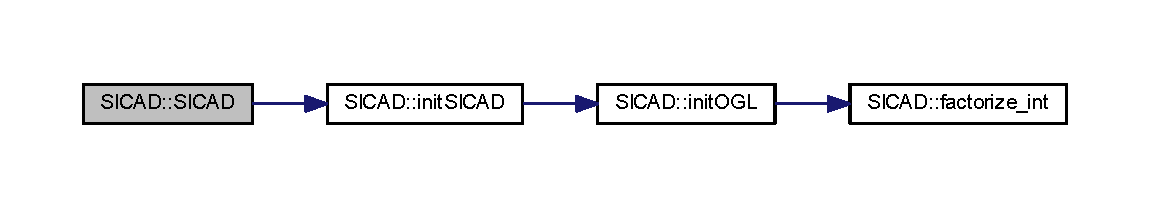
\includegraphics[width=350pt]{classSICAD_abcb9bb154f73472447affb9bb16dcec7_cgraph}
\end{center}
\end{figure}
\mbox{\Hypertarget{classSICAD_a6ddc65ccbfea740515782c4b0dc25a0c}\label{classSICAD_a6ddc65ccbfea740515782c4b0dc25a0c}} 
\index{S\+I\+C\+AD@{S\+I\+C\+AD}!S\+I\+C\+AD@{S\+I\+C\+AD}}
\index{S\+I\+C\+AD@{S\+I\+C\+AD}!S\+I\+C\+AD@{S\+I\+C\+AD}}
\subsubsection{\texorpdfstring{S\+I\+C\+A\+D()}{SICAD()}\hspace{0.1cm}{\footnotesize\ttfamily [7/9]}}
{\footnotesize\ttfamily S\+I\+C\+A\+D\+::\+S\+I\+C\+AD (\begin{DoxyParamCaption}\item[{const \mbox{\hyperlink{classSICAD_a9e1e1460d4c0f331b4fd015aae4dd721}{Model\+Path\+Container}} \&}]{objfile\+\_\+map,  }\item[{const G\+Lsizei}]{cam\+\_\+width,  }\item[{const G\+Lsizei}]{cam\+\_\+height,  }\item[{const G\+Lfloat}]{cam\+\_\+fx,  }\item[{const G\+Lfloat}]{cam\+\_\+fy,  }\item[{const G\+Lfloat}]{cam\+\_\+cx,  }\item[{const G\+Lfloat}]{cam\+\_\+cy,  }\item[{const std\+::string \&}]{shader\+\_\+folder,  }\item[{const bool}]{window\+\_\+visible }\end{DoxyParamCaption})}



Definition at line 85 of file S\+I\+C\+A\+D.\+cpp.

\mbox{\Hypertarget{classSICAD_a1d217cbdc1670f8c5885c413e4acbede}\label{classSICAD_a1d217cbdc1670f8c5885c413e4acbede}} 
\index{S\+I\+C\+AD@{S\+I\+C\+AD}!S\+I\+C\+AD@{S\+I\+C\+AD}}
\index{S\+I\+C\+AD@{S\+I\+C\+AD}!S\+I\+C\+AD@{S\+I\+C\+AD}}
\subsubsection{\texorpdfstring{S\+I\+C\+A\+D()}{SICAD()}\hspace{0.1cm}{\footnotesize\ttfamily [8/9]}}
{\footnotesize\ttfamily S\+I\+C\+A\+D\+::\+S\+I\+C\+AD (\begin{DoxyParamCaption}\item[{const \mbox{\hyperlink{classSICAD_a9e1e1460d4c0f331b4fd015aae4dd721}{Model\+Path\+Container}} \&}]{objfile\+\_\+map,  }\item[{const G\+Lsizei}]{cam\+\_\+width,  }\item[{const G\+Lsizei}]{cam\+\_\+height,  }\item[{const G\+Lfloat}]{cam\+\_\+fx,  }\item[{const G\+Lfloat}]{cam\+\_\+fy,  }\item[{const G\+Lfloat}]{cam\+\_\+cx,  }\item[{const G\+Lfloat}]{cam\+\_\+cy,  }\item[{const G\+Lint}]{num\+\_\+images,  }\item[{const std\+::string \&}]{shader\+\_\+folder,  }\item[{const bool}]{window\+\_\+visible }\end{DoxyParamCaption})}



Definition at line 102 of file S\+I\+C\+A\+D.\+cpp.

\mbox{\Hypertarget{classSICAD_ac4e6349b361e3ec41d828e0d0f77f12b}\label{classSICAD_ac4e6349b361e3ec41d828e0d0f77f12b}} 
\index{S\+I\+C\+AD@{S\+I\+C\+AD}!S\+I\+C\+AD@{S\+I\+C\+AD}}
\index{S\+I\+C\+AD@{S\+I\+C\+AD}!S\+I\+C\+AD@{S\+I\+C\+AD}}
\subsubsection{\texorpdfstring{S\+I\+C\+A\+D()}{SICAD()}\hspace{0.1cm}{\footnotesize\ttfamily [9/9]}}
{\footnotesize\ttfamily S\+I\+C\+A\+D\+::\+S\+I\+C\+AD (\begin{DoxyParamCaption}\item[{const \mbox{\hyperlink{classSICAD_a9e1e1460d4c0f331b4fd015aae4dd721}{Model\+Path\+Container}} \&}]{objfile\+\_\+map,  }\item[{const G\+Lsizei}]{cam\+\_\+width,  }\item[{const G\+Lsizei}]{cam\+\_\+height,  }\item[{const G\+Lfloat}]{cam\+\_\+fx,  }\item[{const G\+Lfloat}]{cam\+\_\+fy,  }\item[{const G\+Lfloat}]{cam\+\_\+cx,  }\item[{const G\+Lfloat}]{cam\+\_\+cy,  }\item[{const G\+Lint}]{num\+\_\+images,  }\item[{const std\+::vector$<$ float $>$ \&}]{ogl\+\_\+to\+\_\+cam,  }\item[{const std\+::string \&}]{shader\+\_\+folder,  }\item[{const bool}]{window\+\_\+visible }\end{DoxyParamCaption})}



Create a \mbox{\hyperlink{classSICAD}{S\+I\+C\+AD}} object with a dedicated Open\+GL window and context. 

For the \mbox{\hyperlink{classSICAD}{S\+I\+C\+AD}} object to work properly, four shaders are needed. Further, their name must be as follows\+:


\begin{DoxyItemize}
\item shader\+\_\+model.\+vert for the model vertex shader
\item shader\+\_\+model.\+frag for the model fragment shader
\item shader\+\_\+background.\+vert for the background vertex shader
\item shader\+\_\+background.\+frag for the background fragment shader
\end{DoxyItemize}


\begin{DoxyParams}{Parameters}
{\em objfile\+\_\+map} & a (tag, path) container to associate a \textquotesingle{}tag\textquotesingle{} to the mesh file specified in \textquotesingle{}path\textquotesingle{}. \\
\hline
{\em cam\+\_\+width} & camera or image width. \\
\hline
{\em cam\+\_\+height} & camera or image height. \\
\hline
{\em cam\+\_\+fx} & focal length along the x axis in pixels. \\
\hline
{\em cam\+\_\+fy} & focal length along the y axis in pixels. \\
\hline
{\em num\+\_\+images} & number of images to render (using gl\+Scissor) in the same window and context. \\
\hline
{\em ogl\+\_\+to\+\_\+cam} & a 7 component pose vector, (x, y, z) position and a (ux, uy, uz, theta) axis-\/angle orientation, defining a camera rotation to be applied to the Open\+GL camera. \\
\hline
{\em shader\+\_\+folder} & folder path containing four shaders, two for the background and two for the mesh. \\
\hline
{\em window\+\_\+visible} & true to show the rendering window, false to perform off-\/screen rendering. \\
\hline
\end{DoxyParams}


Definition at line 120 of file S\+I\+C\+A\+D.\+cpp.



References log\+\_\+\+I\+D\+\_\+, and set\+Projection\+Matrix().

Here is the call graph for this function\+:
\nopagebreak
\begin{figure}[H]
\begin{center}
\leavevmode
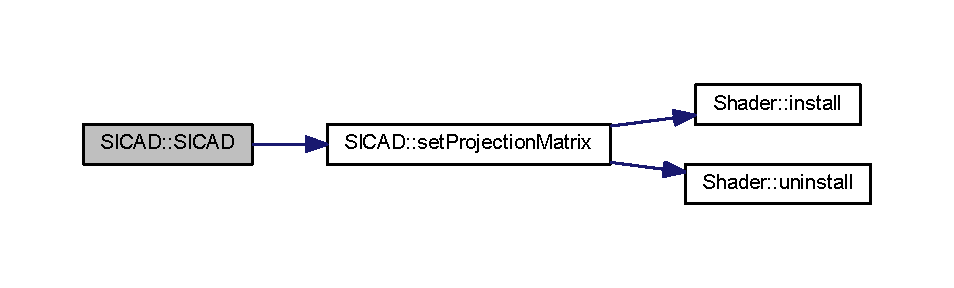
\includegraphics[width=350pt]{classSICAD_ac4e6349b361e3ec41d828e0d0f77f12b_cgraph}
\end{center}
\end{figure}
\mbox{\Hypertarget{classSICAD_a4e3d6d1f90ea2261dcd8507ee8709360}\label{classSICAD_a4e3d6d1f90ea2261dcd8507ee8709360}} 
\index{S\+I\+C\+AD@{S\+I\+C\+AD}!````~S\+I\+C\+AD@{$\sim$\+S\+I\+C\+AD}}
\index{````~S\+I\+C\+AD@{$\sim$\+S\+I\+C\+AD}!S\+I\+C\+AD@{S\+I\+C\+AD}}
\subsubsection{\texorpdfstring{$\sim$\+S\+I\+C\+A\+D()}{~SICAD()}}
{\footnotesize\ttfamily S\+I\+C\+A\+D\+::$\sim$\+S\+I\+C\+AD (\begin{DoxyParamCaption}{ }\end{DoxyParamCaption})\hspace{0.3cm}{\ttfamily [virtual]}}



Definition at line 140 of file S\+I\+C\+A\+D.\+cpp.



References class\+\_\+counter\+\_\+, ebo\+\_\+background\+\_\+, fbo\+\_\+, log\+\_\+\+I\+D\+\_\+, model\+\_\+obj\+\_\+, shader\+\_\+background\+\_\+, shader\+\_\+cad\+\_\+, texture\+\_\+background\+\_\+, texture\+\_\+color\+\_\+buffer\+\_\+, texture\+\_\+depth\+\_\+buffer\+\_\+, vao\+\_\+background\+\_\+, vao\+\_\+frame\+\_\+, vbo\+\_\+background\+\_\+, vbo\+\_\+frame\+\_\+, and window\+\_\+.



\subsection{Member Function Documentation}
\mbox{\Hypertarget{classSICAD_ae2d8d44b5bbcf7329e180aafda2df386}\label{classSICAD_ae2d8d44b5bbcf7329e180aafda2df386}} 
\index{S\+I\+C\+AD@{S\+I\+C\+AD}!callback\+Keypress@{callback\+Keypress}}
\index{callback\+Keypress@{callback\+Keypress}!S\+I\+C\+AD@{S\+I\+C\+AD}}
\subsubsection{\texorpdfstring{callback\+Keypress()}{callbackKeypress()}}
{\footnotesize\ttfamily static void S\+I\+C\+A\+D\+::callback\+Keypress (\begin{DoxyParamCaption}\item[{G\+L\+F\+Wwindow $\ast$}]{window,  }\item[{int}]{key,  }\item[{int}]{scancode,  }\item[{int}]{action,  }\item[{int}]{mode }\end{DoxyParamCaption})\hspace{0.3cm}{\ttfamily [static]}, {\ttfamily [private]}}

\mbox{\Hypertarget{classSICAD_a2603ec5cb9a31bc7be0a335ef513ab0d}\label{classSICAD_a2603ec5cb9a31bc7be0a335ef513ab0d}} 
\index{S\+I\+C\+AD@{S\+I\+C\+AD}!factorize\+\_\+int@{factorize\+\_\+int}}
\index{factorize\+\_\+int@{factorize\+\_\+int}!S\+I\+C\+AD@{S\+I\+C\+AD}}
\subsubsection{\texorpdfstring{factorize\+\_\+int()}{factorize\_int()}}
{\footnotesize\ttfamily void S\+I\+C\+A\+D\+::factorize\+\_\+int (\begin{DoxyParamCaption}\item[{const G\+Lsizei}]{area,  }\item[{const G\+Lsizei}]{width\+\_\+limit,  }\item[{const G\+Lsizei}]{height\+\_\+limit,  }\item[{G\+Lsizei \&}]{width,  }\item[{G\+Lsizei \&}]{height }\end{DoxyParamCaption})\hspace{0.3cm}{\ttfamily [private]}}



Definition at line 942 of file S\+I\+C\+A\+D.\+cpp.



Referenced by init\+O\+G\+L().

\mbox{\Hypertarget{classSICAD_a170bd325654aed9eb81062ac610608fa}\label{classSICAD_a170bd325654aed9eb81062ac610608fa}} 
\index{S\+I\+C\+AD@{S\+I\+C\+AD}!get\+Background\+Opt@{get\+Background\+Opt}}
\index{get\+Background\+Opt@{get\+Background\+Opt}!S\+I\+C\+AD@{S\+I\+C\+AD}}
\subsubsection{\texorpdfstring{get\+Background\+Opt()}{getBackgroundOpt()}}
{\footnotesize\ttfamily bool S\+I\+C\+A\+D\+::get\+Background\+Opt (\begin{DoxyParamCaption}{ }\end{DoxyParamCaption}) const}



Definition at line 834 of file S\+I\+C\+A\+D.\+cpp.



References show\+\_\+background\+\_\+.



Referenced by superimpose().

\mbox{\Hypertarget{classSICAD_a8033a99745f595ea5205e3830cabc389}\label{classSICAD_a8033a99745f595ea5205e3830cabc389}} 
\index{S\+I\+C\+AD@{S\+I\+C\+AD}!get\+Mipmaps\+Opt@{get\+Mipmaps\+Opt}}
\index{get\+Mipmaps\+Opt@{get\+Mipmaps\+Opt}!S\+I\+C\+AD@{S\+I\+C\+AD}}
\subsubsection{\texorpdfstring{get\+Mipmaps\+Opt()}{getMipmapsOpt()}}
{\footnotesize\ttfamily \mbox{\hyperlink{classSICAD_a7e092dede6f660355462d6d548214198}{S\+I\+C\+A\+D\+::\+M\+I\+P\+Maps}} S\+I\+C\+A\+D\+::get\+Mipmaps\+Opt (\begin{DoxyParamCaption}{ }\end{DoxyParamCaption}) const}



Definition at line 853 of file S\+I\+C\+A\+D.\+cpp.



References mesh\+\_\+mmaps\+\_\+.



Referenced by set\+Background().

\mbox{\Hypertarget{classSICAD_aaf003ab2ac8bc5ebdef6611ca1547e73}\label{classSICAD_aaf003ab2ac8bc5ebdef6611ca1547e73}} 
\index{S\+I\+C\+AD@{S\+I\+C\+AD}!get\+Ogl\+Window\+Should\+Close@{get\+Ogl\+Window\+Should\+Close}}
\index{get\+Ogl\+Window\+Should\+Close@{get\+Ogl\+Window\+Should\+Close}!S\+I\+C\+AD@{S\+I\+C\+AD}}
\subsubsection{\texorpdfstring{get\+Ogl\+Window\+Should\+Close()}{getOglWindowShouldClose()}}
{\footnotesize\ttfamily bool S\+I\+C\+A\+D\+::get\+Ogl\+Window\+Should\+Close (\begin{DoxyParamCaption}{ }\end{DoxyParamCaption})}



Definition at line 500 of file S\+I\+C\+A\+D.\+cpp.



References is\+\_\+initialized\+\_\+, and window\+\_\+.

\mbox{\Hypertarget{classSICAD_a2ba3a0aeb3dab9996bdeed19a16eae56}\label{classSICAD_a2ba3a0aeb3dab9996bdeed19a16eae56}} 
\index{S\+I\+C\+AD@{S\+I\+C\+AD}!get\+Tiles\+Cols@{get\+Tiles\+Cols}}
\index{get\+Tiles\+Cols@{get\+Tiles\+Cols}!S\+I\+C\+AD@{S\+I\+C\+AD}}
\subsubsection{\texorpdfstring{get\+Tiles\+Cols()}{getTilesCols()}}
{\footnotesize\ttfamily int S\+I\+C\+A\+D\+::get\+Tiles\+Cols (\begin{DoxyParamCaption}{ }\end{DoxyParamCaption}) const}



Definition at line 871 of file S\+I\+C\+A\+D.\+cpp.



References tiles\+\_\+cols\+\_\+.

\mbox{\Hypertarget{classSICAD_a728f82ebbfeea54f3fef2fc0c56a4964}\label{classSICAD_a728f82ebbfeea54f3fef2fc0c56a4964}} 
\index{S\+I\+C\+AD@{S\+I\+C\+AD}!get\+Tiles\+Number@{get\+Tiles\+Number}}
\index{get\+Tiles\+Number@{get\+Tiles\+Number}!S\+I\+C\+AD@{S\+I\+C\+AD}}
\subsubsection{\texorpdfstring{get\+Tiles\+Number()}{getTilesNumber()}}
{\footnotesize\ttfamily int S\+I\+C\+A\+D\+::get\+Tiles\+Number (\begin{DoxyParamCaption}{ }\end{DoxyParamCaption}) const}



Definition at line 859 of file S\+I\+C\+A\+D.\+cpp.



References tiles\+\_\+cols\+\_\+, and tiles\+\_\+rows\+\_\+.

\mbox{\Hypertarget{classSICAD_a9e3dd48dfd83ea0bd00d64dacc4fbd40}\label{classSICAD_a9e3dd48dfd83ea0bd00d64dacc4fbd40}} 
\index{S\+I\+C\+AD@{S\+I\+C\+AD}!get\+Tiles\+Rows@{get\+Tiles\+Rows}}
\index{get\+Tiles\+Rows@{get\+Tiles\+Rows}!S\+I\+C\+AD@{S\+I\+C\+AD}}
\subsubsection{\texorpdfstring{get\+Tiles\+Rows()}{getTilesRows()}}
{\footnotesize\ttfamily int S\+I\+C\+A\+D\+::get\+Tiles\+Rows (\begin{DoxyParamCaption}{ }\end{DoxyParamCaption}) const}



Definition at line 865 of file S\+I\+C\+A\+D.\+cpp.



References tiles\+\_\+rows\+\_\+.

\mbox{\Hypertarget{classSICAD_a1bdece095865249df4cb4e6a7ad2901e}\label{classSICAD_a1bdece095865249df4cb4e6a7ad2901e}} 
\index{S\+I\+C\+AD@{S\+I\+C\+AD}!get\+View\+Transformation\+Matrix@{get\+View\+Transformation\+Matrix}}
\index{get\+View\+Transformation\+Matrix@{get\+View\+Transformation\+Matrix}!S\+I\+C\+AD@{S\+I\+C\+AD}}
\subsubsection{\texorpdfstring{get\+View\+Transformation\+Matrix()}{getViewTransformationMatrix()}}
{\footnotesize\ttfamily glm\+::mat4 S\+I\+C\+A\+D\+::get\+View\+Transformation\+Matrix (\begin{DoxyParamCaption}\item[{const double $\ast$}]{cam\+\_\+x,  }\item[{const double $\ast$}]{cam\+\_\+o }\end{DoxyParamCaption})\hspace{0.3cm}{\ttfamily [private]}}



Definition at line 877 of file S\+I\+C\+A\+D.\+cpp.



References ogl\+\_\+to\+\_\+cam\+\_\+.



Referenced by superimpose().

\mbox{\Hypertarget{classSICAD_af65b5ad73e2c0e872face157b56bd68b}\label{classSICAD_af65b5ad73e2c0e872face157b56bd68b}} 
\index{S\+I\+C\+AD@{S\+I\+C\+AD}!get\+Wireframe\+Opt@{get\+Wireframe\+Opt}}
\index{get\+Wireframe\+Opt@{get\+Wireframe\+Opt}!S\+I\+C\+AD@{S\+I\+C\+AD}}
\subsubsection{\texorpdfstring{get\+Wireframe\+Opt()}{getWireframeOpt()}}
{\footnotesize\ttfamily G\+Lenum S\+I\+C\+A\+D\+::get\+Wireframe\+Opt (\begin{DoxyParamCaption}{ }\end{DoxyParamCaption}) const}



Definition at line 847 of file S\+I\+C\+A\+D.\+cpp.



References show\+\_\+mesh\+\_\+mode\+\_\+.



Referenced by superimpose().

\mbox{\Hypertarget{classSICAD_a102619690ab32e300405d22d52e36a5e}\label{classSICAD_a102619690ab32e300405d22d52e36a5e}} 
\index{S\+I\+C\+AD@{S\+I\+C\+AD}!init\+O\+GL@{init\+O\+GL}}
\index{init\+O\+GL@{init\+O\+GL}!S\+I\+C\+AD@{S\+I\+C\+AD}}
\subsubsection{\texorpdfstring{init\+O\+G\+L()}{initOGL()}}
{\footnotesize\ttfamily bool S\+I\+C\+A\+D\+::init\+O\+GL (\begin{DoxyParamCaption}\item[{const G\+Lsizei}]{width,  }\item[{const G\+Lsizei}]{height,  }\item[{const G\+Lint}]{num\+\_\+viewports,  }\item[{const bool}]{window\+\_\+visibile }\end{DoxyParamCaption})\hspace{0.3cm}{\ttfamily [private]}}



Definition at line 413 of file S\+I\+C\+A\+D.\+cpp.



References factorize\+\_\+int(), framebuffer\+\_\+height\+\_\+, framebuffer\+\_\+width\+\_\+, image\+\_\+height\+\_\+, image\+\_\+width\+\_\+, log\+\_\+\+I\+D\+\_\+, main\+\_\+thread\+\_\+id\+\_\+, render\+\_\+img\+\_\+height\+\_\+, render\+\_\+img\+\_\+width\+\_\+, renderbuffer\+\_\+size\+\_\+, tiles\+\_\+cols\+\_\+, tiles\+\_\+num\+\_\+, tiles\+\_\+rows\+\_\+, and window\+\_\+.



Referenced by init\+S\+I\+C\+A\+D().

Here is the call graph for this function\+:
\nopagebreak
\begin{figure}[H]
\begin{center}
\leavevmode
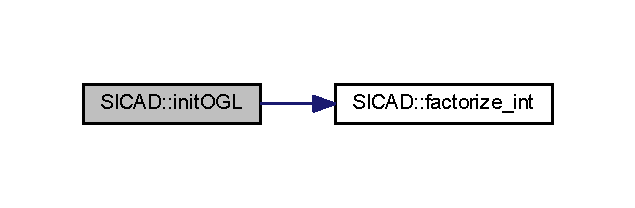
\includegraphics[width=305pt]{classSICAD_a102619690ab32e300405d22d52e36a5e_cgraph}
\end{center}
\end{figure}
\mbox{\Hypertarget{classSICAD_a04e1291dc1a51b2dee87dbe9a5b3a316}\label{classSICAD_a04e1291dc1a51b2dee87dbe9a5b3a316}} 
\index{S\+I\+C\+AD@{S\+I\+C\+AD}!init\+S\+I\+C\+AD@{init\+S\+I\+C\+AD}}
\index{init\+S\+I\+C\+AD@{init\+S\+I\+C\+AD}!S\+I\+C\+AD@{S\+I\+C\+AD}}
\subsubsection{\texorpdfstring{init\+S\+I\+C\+A\+D()}{initSICAD()}\hspace{0.1cm}{\footnotesize\ttfamily [1/2]}}
{\footnotesize\ttfamily bool S\+I\+C\+A\+D\+::init\+S\+I\+C\+AD (\begin{DoxyParamCaption}\item[{const \mbox{\hyperlink{classSICAD_a9e1e1460d4c0f331b4fd015aae4dd721}{Model\+Path\+Container}} \&}]{objfile\+\_\+map,  }\item[{const G\+Lsizei}]{cam\+\_\+width,  }\item[{const G\+Lsizei}]{cam\+\_\+height,  }\item[{const G\+Lint}]{num\+\_\+images,  }\item[{const std\+::vector$<$ float $>$ \&}]{ogl\+\_\+to\+\_\+cam,  }\item[{const std\+::string \&}]{shader\+\_\+folder,  }\item[{const bool}]{window\+\_\+visible }\end{DoxyParamCaption})}



Definition at line 181 of file S\+I\+C\+A\+D.\+cpp.



References back\+\_\+proj\+\_\+, class\+\_\+counter\+\_\+, ebo\+\_\+background\+\_\+, far\+\_\+, fbo\+\_\+, framebuffer\+\_\+height\+\_\+, framebuffer\+\_\+width\+\_\+, init\+O\+G\+L(), is\+\_\+initialized\+\_\+, log\+\_\+\+I\+D\+\_\+, model\+\_\+obj\+\_\+, ogl\+\_\+to\+\_\+cam\+\_\+, shader\+\_\+background\+\_\+, shader\+\_\+cad\+\_\+, shader\+\_\+frame\+\_\+, texture\+\_\+background\+\_\+, texture\+\_\+color\+\_\+buffer\+\_\+, texture\+\_\+depth\+\_\+buffer\+\_\+, vao\+\_\+background\+\_\+, vao\+\_\+frame\+\_\+, vbo\+\_\+background\+\_\+, vbo\+\_\+frame\+\_\+, and window\+\_\+.



Referenced by init\+S\+I\+C\+A\+D(), and S\+I\+C\+A\+D().

Here is the call graph for this function\+:
\nopagebreak
\begin{figure}[H]
\begin{center}
\leavevmode
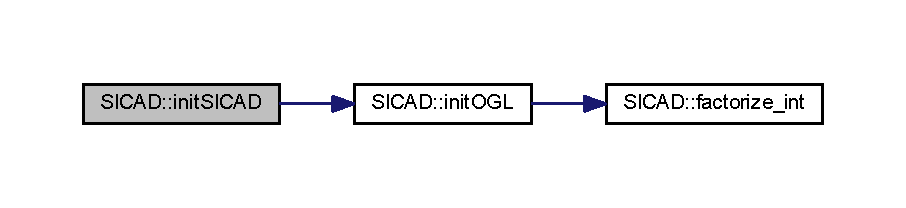
\includegraphics[width=350pt]{classSICAD_a04e1291dc1a51b2dee87dbe9a5b3a316_cgraph}
\end{center}
\end{figure}
\mbox{\Hypertarget{classSICAD_abb2b0250a885435828d5255645e06ac8}\label{classSICAD_abb2b0250a885435828d5255645e06ac8}} 
\index{S\+I\+C\+AD@{S\+I\+C\+AD}!init\+S\+I\+C\+AD@{init\+S\+I\+C\+AD}}
\index{init\+S\+I\+C\+AD@{init\+S\+I\+C\+AD}!S\+I\+C\+AD@{S\+I\+C\+AD}}
\subsubsection{\texorpdfstring{init\+S\+I\+C\+A\+D()}{initSICAD()}\hspace{0.1cm}{\footnotesize\ttfamily [2/2]}}
{\footnotesize\ttfamily bool S\+I\+C\+A\+D\+::init\+S\+I\+C\+AD (\begin{DoxyParamCaption}\item[{const \mbox{\hyperlink{classSICAD_a9e1e1460d4c0f331b4fd015aae4dd721}{Model\+Path\+Container}} \&}]{objfile\+\_\+map,  }\item[{const G\+Lsizei}]{cam\+\_\+width,  }\item[{const G\+Lsizei}]{cam\+\_\+height,  }\item[{const G\+Lfloat}]{cam\+\_\+fx,  }\item[{const G\+Lfloat}]{cam\+\_\+fy,  }\item[{const G\+Lfloat}]{cam\+\_\+cx,  }\item[{const G\+Lfloat}]{cam\+\_\+cy,  }\item[{const G\+Lint}]{num\+\_\+images,  }\item[{const std\+::vector$<$ float $>$ \&}]{ogl\+\_\+to\+\_\+cam,  }\item[{const std\+::string \&}]{shader\+\_\+folder,  }\item[{const bool}]{window\+\_\+visible }\end{DoxyParamCaption})}



Definition at line 389 of file S\+I\+C\+A\+D.\+cpp.



References init\+S\+I\+C\+A\+D(), log\+\_\+\+I\+D\+\_\+, and set\+Projection\+Matrix().

Here is the call graph for this function\+:
\nopagebreak
\begin{figure}[H]
\begin{center}
\leavevmode
\includegraphics[width=350pt]{classSICAD_abb2b0250a885435828d5255645e06ac8_cgraph}
\end{center}
\end{figure}
\mbox{\Hypertarget{classSICAD_a8238a2b2c488c8b7ba85d5b2a0bf00ac}\label{classSICAD_a8238a2b2c488c8b7ba85d5b2a0bf00ac}} 
\index{S\+I\+C\+AD@{S\+I\+C\+AD}!poll\+Or\+Post\+Event@{poll\+Or\+Post\+Event}}
\index{poll\+Or\+Post\+Event@{poll\+Or\+Post\+Event}!S\+I\+C\+AD@{S\+I\+C\+AD}}
\subsubsection{\texorpdfstring{poll\+Or\+Post\+Event()}{pollOrPostEvent()}}
{\footnotesize\ttfamily void S\+I\+C\+A\+D\+::poll\+Or\+Post\+Event (\begin{DoxyParamCaption}{ }\end{DoxyParamCaption})\hspace{0.3cm}{\ttfamily [private]}}



Definition at line 892 of file S\+I\+C\+A\+D.\+cpp.



References main\+\_\+thread\+\_\+id\+\_\+.



Referenced by set\+Ogl\+Window\+Should\+Close(), and superimpose().

\mbox{\Hypertarget{classSICAD_a25b180f54f2e93d69b291cc225600c8e}\label{classSICAD_a25b180f54f2e93d69b291cc225600c8e}} 
\index{S\+I\+C\+AD@{S\+I\+C\+AD}!set\+Background@{set\+Background}}
\index{set\+Background@{set\+Background}!S\+I\+C\+AD@{S\+I\+C\+AD}}
\subsubsection{\texorpdfstring{set\+Background()}{setBackground()}}
{\footnotesize\ttfamily void S\+I\+C\+A\+D\+::set\+Background (\begin{DoxyParamCaption}\item[{cv\+::\+Mat \&}]{img }\end{DoxyParamCaption})\hspace{0.3cm}{\ttfamily [private]}}



Definition at line 901 of file S\+I\+C\+A\+D.\+cpp.



References back\+\_\+proj\+\_\+, get\+Mipmaps\+Opt(), Shader\+::install(), linear, nearest, Shader\+::\+Program, shader\+\_\+background\+\_\+, texture\+\_\+background\+\_\+, Shader\+::uninstall(), and vao\+\_\+background\+\_\+.



Referenced by superimpose().

Here is the call graph for this function\+:
\nopagebreak
\begin{figure}[H]
\begin{center}
\leavevmode
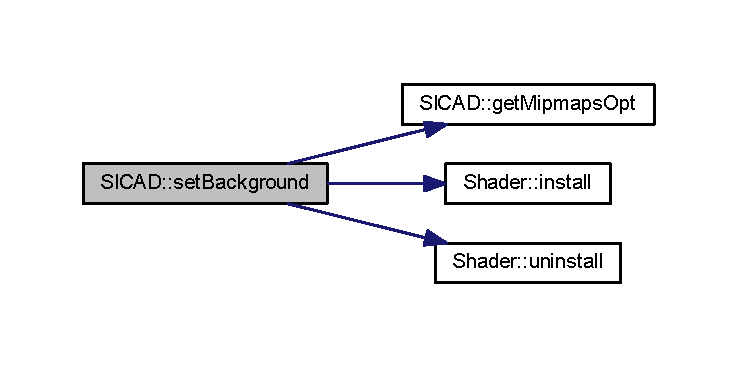
\includegraphics[width=350pt]{classSICAD_a25b180f54f2e93d69b291cc225600c8e_cgraph}
\end{center}
\end{figure}
\mbox{\Hypertarget{classSICAD_a07921943ad3d4016dcbe76135e799754}\label{classSICAD_a07921943ad3d4016dcbe76135e799754}} 
\index{S\+I\+C\+AD@{S\+I\+C\+AD}!set\+Background\+Opt@{set\+Background\+Opt}}
\index{set\+Background\+Opt@{set\+Background\+Opt}!S\+I\+C\+AD@{S\+I\+C\+AD}}
\subsubsection{\texorpdfstring{set\+Background\+Opt()}{setBackgroundOpt()}}
{\footnotesize\ttfamily void S\+I\+C\+A\+D\+::set\+Background\+Opt (\begin{DoxyParamCaption}\item[{bool}]{show\+\_\+background }\end{DoxyParamCaption})}



Definition at line 828 of file S\+I\+C\+A\+D.\+cpp.



References show\+\_\+background\+\_\+.



Referenced by main().

\mbox{\Hypertarget{classSICAD_a0e42acab32252ddc878794f365ee1037}\label{classSICAD_a0e42acab32252ddc878794f365ee1037}} 
\index{S\+I\+C\+AD@{S\+I\+C\+AD}!set\+Ogl\+Window\+Should\+Close@{set\+Ogl\+Window\+Should\+Close}}
\index{set\+Ogl\+Window\+Should\+Close@{set\+Ogl\+Window\+Should\+Close}!S\+I\+C\+AD@{S\+I\+C\+AD}}
\subsubsection{\texorpdfstring{set\+Ogl\+Window\+Should\+Close()}{setOglWindowShouldClose()}}
{\footnotesize\ttfamily void S\+I\+C\+A\+D\+::set\+Ogl\+Window\+Should\+Close (\begin{DoxyParamCaption}\item[{bool}]{should\+\_\+close }\end{DoxyParamCaption})}



Definition at line 512 of file S\+I\+C\+A\+D.\+cpp.



References is\+\_\+initialized\+\_\+, poll\+Or\+Post\+Event(), and window\+\_\+.

Here is the call graph for this function\+:
\nopagebreak
\begin{figure}[H]
\begin{center}
\leavevmode
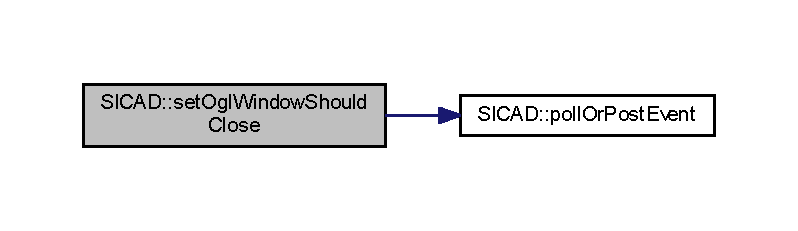
\includegraphics[width=350pt]{classSICAD_a0e42acab32252ddc878794f365ee1037_cgraph}
\end{center}
\end{figure}
\mbox{\Hypertarget{classSICAD_a39cdff6871d32429d8ba95b776e0b874}\label{classSICAD_a39cdff6871d32429d8ba95b776e0b874}} 
\index{S\+I\+C\+AD@{S\+I\+C\+AD}!set\+Projection\+Matrix@{set\+Projection\+Matrix}}
\index{set\+Projection\+Matrix@{set\+Projection\+Matrix}!S\+I\+C\+AD@{S\+I\+C\+AD}}
\subsubsection{\texorpdfstring{set\+Projection\+Matrix()}{setProjectionMatrix()}}
{\footnotesize\ttfamily bool S\+I\+C\+A\+D\+::set\+Projection\+Matrix (\begin{DoxyParamCaption}\item[{const G\+Lsizei}]{cam\+\_\+width,  }\item[{const G\+Lsizei}]{cam\+\_\+height,  }\item[{const G\+Lfloat}]{cam\+\_\+fx,  }\item[{const G\+Lfloat}]{cam\+\_\+fy,  }\item[{const G\+Lfloat}]{cam\+\_\+cx,  }\item[{const G\+Lfloat}]{cam\+\_\+cy }\end{DoxyParamCaption})}



Definition at line 774 of file S\+I\+C\+A\+D.\+cpp.



References far\+\_\+, has\+\_\+proj\+\_\+matrix\+\_\+, Shader\+::install(), is\+\_\+initialized\+\_\+, near\+\_\+, Shader\+::\+Program, projection\+\_\+, shader\+\_\+cad\+\_\+, shader\+\_\+frame\+\_\+, Shader\+::uninstall(), and window\+\_\+.



Referenced by init\+S\+I\+C\+A\+D(), S\+I\+C\+A\+D(), and superimpose().

Here is the call graph for this function\+:
\nopagebreak
\begin{figure}[H]
\begin{center}
\leavevmode
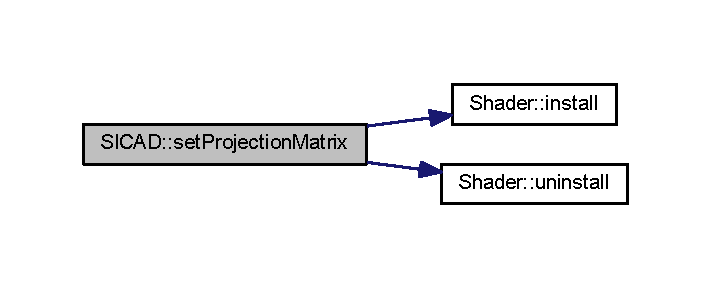
\includegraphics[width=341pt]{classSICAD_a39cdff6871d32429d8ba95b776e0b874_cgraph}
\end{center}
\end{figure}
\mbox{\Hypertarget{classSICAD_ae7af7aba5d81b9f1cc3e273a55811a70}\label{classSICAD_ae7af7aba5d81b9f1cc3e273a55811a70}} 
\index{S\+I\+C\+AD@{S\+I\+C\+AD}!set\+Wireframe@{set\+Wireframe}}
\index{set\+Wireframe@{set\+Wireframe}!S\+I\+C\+AD@{S\+I\+C\+AD}}
\subsubsection{\texorpdfstring{set\+Wireframe()}{setWireframe()}}
{\footnotesize\ttfamily void S\+I\+C\+A\+D\+::set\+Wireframe (\begin{DoxyParamCaption}\item[{G\+Lenum}]{mode }\end{DoxyParamCaption})\hspace{0.3cm}{\ttfamily [private]}}



Definition at line 936 of file S\+I\+C\+A\+D.\+cpp.



Referenced by superimpose().

\mbox{\Hypertarget{classSICAD_a4cf80a273b6b0d946cd298472c63ddd4}\label{classSICAD_a4cf80a273b6b0d946cd298472c63ddd4}} 
\index{S\+I\+C\+AD@{S\+I\+C\+AD}!set\+Wireframe\+Opt@{set\+Wireframe\+Opt}}
\index{set\+Wireframe\+Opt@{set\+Wireframe\+Opt}!S\+I\+C\+AD@{S\+I\+C\+AD}}
\subsubsection{\texorpdfstring{set\+Wireframe\+Opt()}{setWireframeOpt()}}
{\footnotesize\ttfamily void S\+I\+C\+A\+D\+::set\+Wireframe\+Opt (\begin{DoxyParamCaption}\item[{bool}]{show\+\_\+mesh\+\_\+wires }\end{DoxyParamCaption})}



Definition at line 840 of file S\+I\+C\+A\+D.\+cpp.



References show\+\_\+mesh\+\_\+mode\+\_\+.

\mbox{\Hypertarget{classSICAD_a356e0ac8a0f130952a72326bedd4ab60}\label{classSICAD_a356e0ac8a0f130952a72326bedd4ab60}} 
\index{S\+I\+C\+AD@{S\+I\+C\+AD}!superimpose@{superimpose}}
\index{superimpose@{superimpose}!S\+I\+C\+AD@{S\+I\+C\+AD}}
\subsubsection{\texorpdfstring{superimpose()}{superimpose()}\hspace{0.1cm}{\footnotesize\ttfamily [1/4]}}
{\footnotesize\ttfamily bool S\+I\+C\+A\+D\+::superimpose (\begin{DoxyParamCaption}\item[{const \mbox{\hyperlink{classSuperimpose_a178e3d4e2def6635bfcf9454dd4b5d22}{Model\+Pose\+Container}} \&}]{objpos\+\_\+map,  }\item[{const double $\ast$}]{cam\+\_\+x,  }\item[{const double $\ast$}]{cam\+\_\+o,  }\item[{cv\+::\+Mat \&}]{img }\end{DoxyParamCaption})\hspace{0.3cm}{\ttfamily [override]}, {\ttfamily [virtual]}}



\mbox{\hyperlink{classSuperimpose}{Superimpose}} one of the mesh models loaded during \mbox{\hyperlink{classSICAD}{S\+I\+C\+AD}} object construction in a given pose from a particular camera viewpoint. 

If the size of cv\+::\+Mat img is not correct to store the result of the superimposition process, it is automatically resized.

\begin{DoxyNote}{Note}
If cv\+::\+Mat img is a background image it must be of size cam\+\_\+width$\ast$cam\+\_\+height, as specified during object construction, and the \mbox{\hyperlink{classSICAD_a07921943ad3d4016dcbe76135e799754}{S\+I\+C\+A\+D\+::set\+Background\+Opt(bool show\+\_\+background)}} must have been evoked with true.
\end{DoxyNote}

\begin{DoxyParams}{Parameters}
{\em objpos\+\_\+map} & a (tag, pose) container to associate a 7 component \textquotesingle{}pose\textquotesingle{}, (x, y, z) position and a (ux, uy, uz, theta) axis-\/angle orientation, to a mesh with tag \textquotesingle{}tag\textquotesingle{}. \\
\hline
{\em cam\+\_\+x} & (x, y, z) position \\
\hline
{\em cam\+\_\+o} & (ux, uy, uz, theta) axis-\/angle orientation \\
\hline
{\em img} & an image where the result of the superimposition is stored\\
\hline
\end{DoxyParams}
\begin{DoxyReturn}{Returns}
true upon success, false otherswise. 
\end{DoxyReturn}


Implements \mbox{\hyperlink{classSuperimpose_a62c4c269b8fc34cc36d3d54fa4acb35c}{Superimpose}}.



Definition at line 526 of file S\+I\+C\+A\+D.\+cpp.



References fbo\+\_\+, framebuffer\+\_\+height\+\_\+, framebuffer\+\_\+width\+\_\+, get\+Background\+Opt(), get\+View\+Transformation\+Matrix(), get\+Wireframe\+Opt(), has\+\_\+proj\+\_\+matrix\+\_\+, Shader\+::install(), is\+\_\+initialized\+\_\+, model\+\_\+obj\+\_\+, poll\+Or\+Post\+Event(), Shader\+::\+Program, render\+\_\+img\+\_\+height\+\_\+, render\+\_\+img\+\_\+width\+\_\+, set\+Background(), set\+Wireframe(), shader\+\_\+cad\+\_\+, shader\+\_\+frame\+\_\+, tiles\+\_\+cols\+\_\+, tiles\+\_\+rows\+\_\+, Shader\+::uninstall(), vao\+\_\+frame\+\_\+, and window\+\_\+.



Referenced by main(), and superimpose().

Here is the call graph for this function\+:
\nopagebreak
\begin{figure}[H]
\begin{center}
\leavevmode
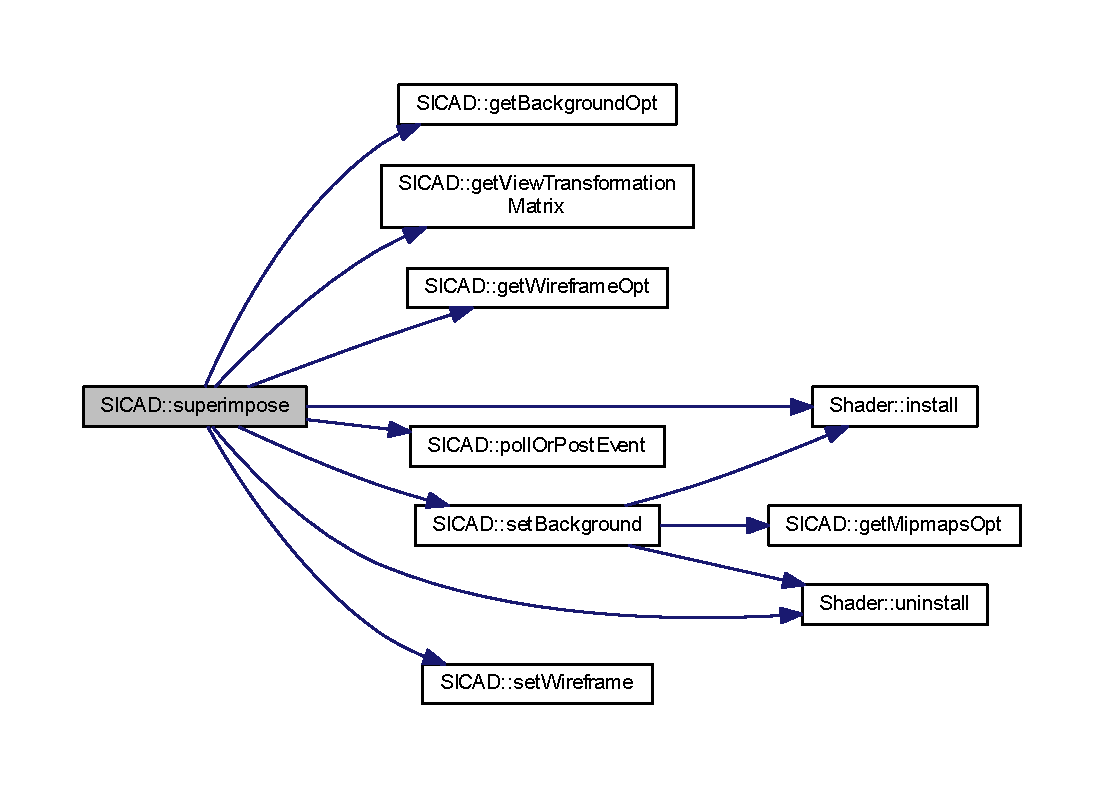
\includegraphics[width=350pt]{classSICAD_a356e0ac8a0f130952a72326bedd4ab60_cgraph}
\end{center}
\end{figure}
\mbox{\Hypertarget{classSICAD_ab15f84cec5a65c8dd6cad85f9b0e1993}\label{classSICAD_ab15f84cec5a65c8dd6cad85f9b0e1993}} 
\index{S\+I\+C\+AD@{S\+I\+C\+AD}!superimpose@{superimpose}}
\index{superimpose@{superimpose}!S\+I\+C\+AD@{S\+I\+C\+AD}}
\subsubsection{\texorpdfstring{superimpose()}{superimpose()}\hspace{0.1cm}{\footnotesize\ttfamily [2/4]}}
{\footnotesize\ttfamily bool S\+I\+C\+A\+D\+::superimpose (\begin{DoxyParamCaption}\item[{const std\+::vector$<$ \mbox{\hyperlink{classSuperimpose_a178e3d4e2def6635bfcf9454dd4b5d22}{Model\+Pose\+Container}} $>$ \&}]{objpos\+\_\+multimap,  }\item[{const double $\ast$}]{cam\+\_\+x,  }\item[{const double $\ast$}]{cam\+\_\+o,  }\item[{cv\+::\+Mat \&}]{img }\end{DoxyParamCaption})\hspace{0.3cm}{\ttfamily [virtual]}}



Definition at line 626 of file S\+I\+C\+A\+D.\+cpp.



References fbo\+\_\+, framebuffer\+\_\+height\+\_\+, framebuffer\+\_\+width\+\_\+, get\+Background\+Opt(), get\+View\+Transformation\+Matrix(), get\+Wireframe\+Opt(), has\+\_\+proj\+\_\+matrix\+\_\+, Shader\+::install(), is\+\_\+initialized\+\_\+, model\+\_\+obj\+\_\+, poll\+Or\+Post\+Event(), Shader\+::\+Program, render\+\_\+img\+\_\+height\+\_\+, render\+\_\+img\+\_\+width\+\_\+, set\+Background(), set\+Wireframe(), shader\+\_\+cad\+\_\+, shader\+\_\+frame\+\_\+, tiles\+\_\+cols\+\_\+, tiles\+\_\+num\+\_\+, tiles\+\_\+rows\+\_\+, Shader\+::uninstall(), vao\+\_\+frame\+\_\+, and window\+\_\+.

Here is the call graph for this function\+:
\nopagebreak
\begin{figure}[H]
\begin{center}
\leavevmode
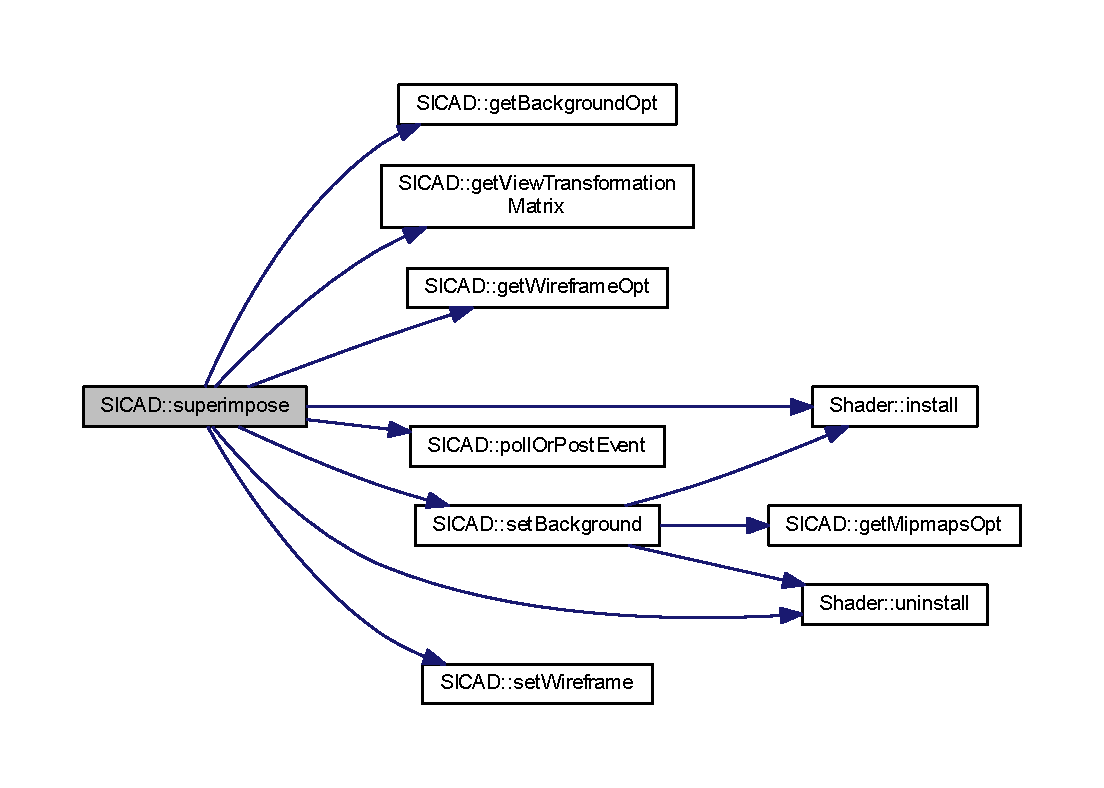
\includegraphics[width=350pt]{classSICAD_ab15f84cec5a65c8dd6cad85f9b0e1993_cgraph}
\end{center}
\end{figure}
\mbox{\Hypertarget{classSICAD_af6c19a679de29992c5f9609f4424add0}\label{classSICAD_af6c19a679de29992c5f9609f4424add0}} 
\index{S\+I\+C\+AD@{S\+I\+C\+AD}!superimpose@{superimpose}}
\index{superimpose@{superimpose}!S\+I\+C\+AD@{S\+I\+C\+AD}}
\subsubsection{\texorpdfstring{superimpose()}{superimpose()}\hspace{0.1cm}{\footnotesize\ttfamily [3/4]}}
{\footnotesize\ttfamily bool S\+I\+C\+A\+D\+::superimpose (\begin{DoxyParamCaption}\item[{const \mbox{\hyperlink{classSuperimpose_a178e3d4e2def6635bfcf9454dd4b5d22}{Model\+Pose\+Container}} \&}]{objpos\+\_\+map,  }\item[{const double $\ast$}]{cam\+\_\+x,  }\item[{const double $\ast$}]{cam\+\_\+o,  }\item[{cv\+::\+Mat \&}]{img,  }\item[{const G\+Lsizei}]{cam\+\_\+width,  }\item[{const G\+Lsizei}]{cam\+\_\+height,  }\item[{const G\+Lfloat}]{cam\+\_\+fx,  }\item[{const G\+Lfloat}]{cam\+\_\+fy,  }\item[{const G\+Lfloat}]{cam\+\_\+cx,  }\item[{const G\+Lfloat}]{cam\+\_\+cy }\end{DoxyParamCaption})\hspace{0.3cm}{\ttfamily [virtual]}}



Definition at line 740 of file S\+I\+C\+A\+D.\+cpp.



References is\+\_\+initialized\+\_\+, set\+Projection\+Matrix(), and superimpose().

Here is the call graph for this function\+:
\nopagebreak
\begin{figure}[H]
\begin{center}
\leavevmode
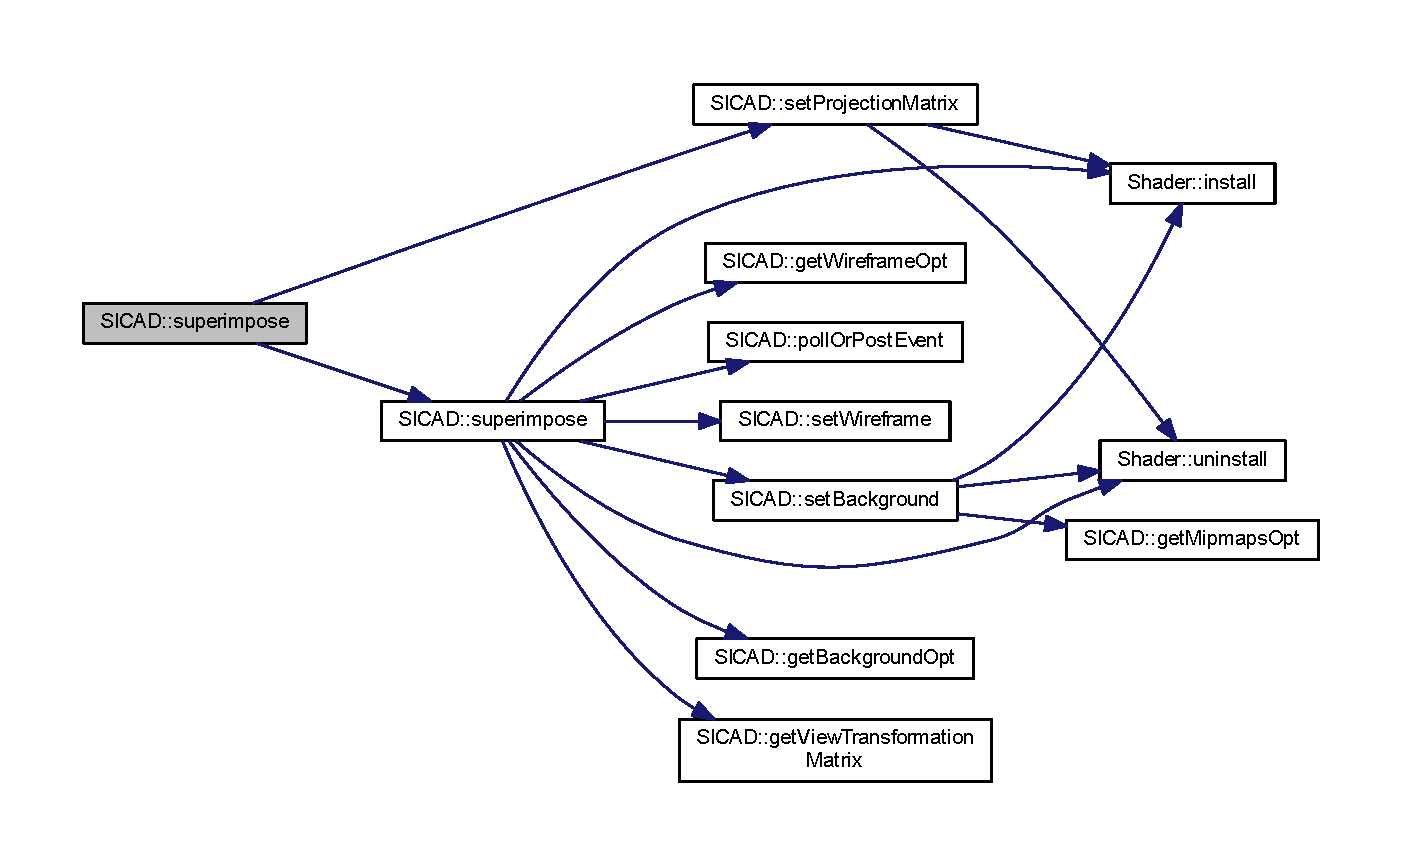
\includegraphics[width=350pt]{classSICAD_af6c19a679de29992c5f9609f4424add0_cgraph}
\end{center}
\end{figure}
\mbox{\Hypertarget{classSICAD_a269e238387393b44177daa4eae88fedd}\label{classSICAD_a269e238387393b44177daa4eae88fedd}} 
\index{S\+I\+C\+AD@{S\+I\+C\+AD}!superimpose@{superimpose}}
\index{superimpose@{superimpose}!S\+I\+C\+AD@{S\+I\+C\+AD}}
\subsubsection{\texorpdfstring{superimpose()}{superimpose()}\hspace{0.1cm}{\footnotesize\ttfamily [4/4]}}
{\footnotesize\ttfamily bool S\+I\+C\+A\+D\+::superimpose (\begin{DoxyParamCaption}\item[{const std\+::vector$<$ \mbox{\hyperlink{classSuperimpose_a178e3d4e2def6635bfcf9454dd4b5d22}{Model\+Pose\+Container}} $>$ \&}]{objpos\+\_\+multimap,  }\item[{const double $\ast$}]{cam\+\_\+x,  }\item[{const double $\ast$}]{cam\+\_\+o,  }\item[{cv\+::\+Mat \&}]{img,  }\item[{const G\+Lsizei}]{cam\+\_\+width,  }\item[{const G\+Lsizei}]{cam\+\_\+height,  }\item[{const G\+Lfloat}]{cam\+\_\+fx,  }\item[{const G\+Lfloat}]{cam\+\_\+fy,  }\item[{const G\+Lfloat}]{cam\+\_\+cx,  }\item[{const G\+Lfloat}]{cam\+\_\+cy }\end{DoxyParamCaption})\hspace{0.3cm}{\ttfamily [virtual]}}



Definition at line 757 of file S\+I\+C\+A\+D.\+cpp.



References is\+\_\+initialized\+\_\+, set\+Projection\+Matrix(), and superimpose().

Here is the call graph for this function\+:
\nopagebreak
\begin{figure}[H]
\begin{center}
\leavevmode
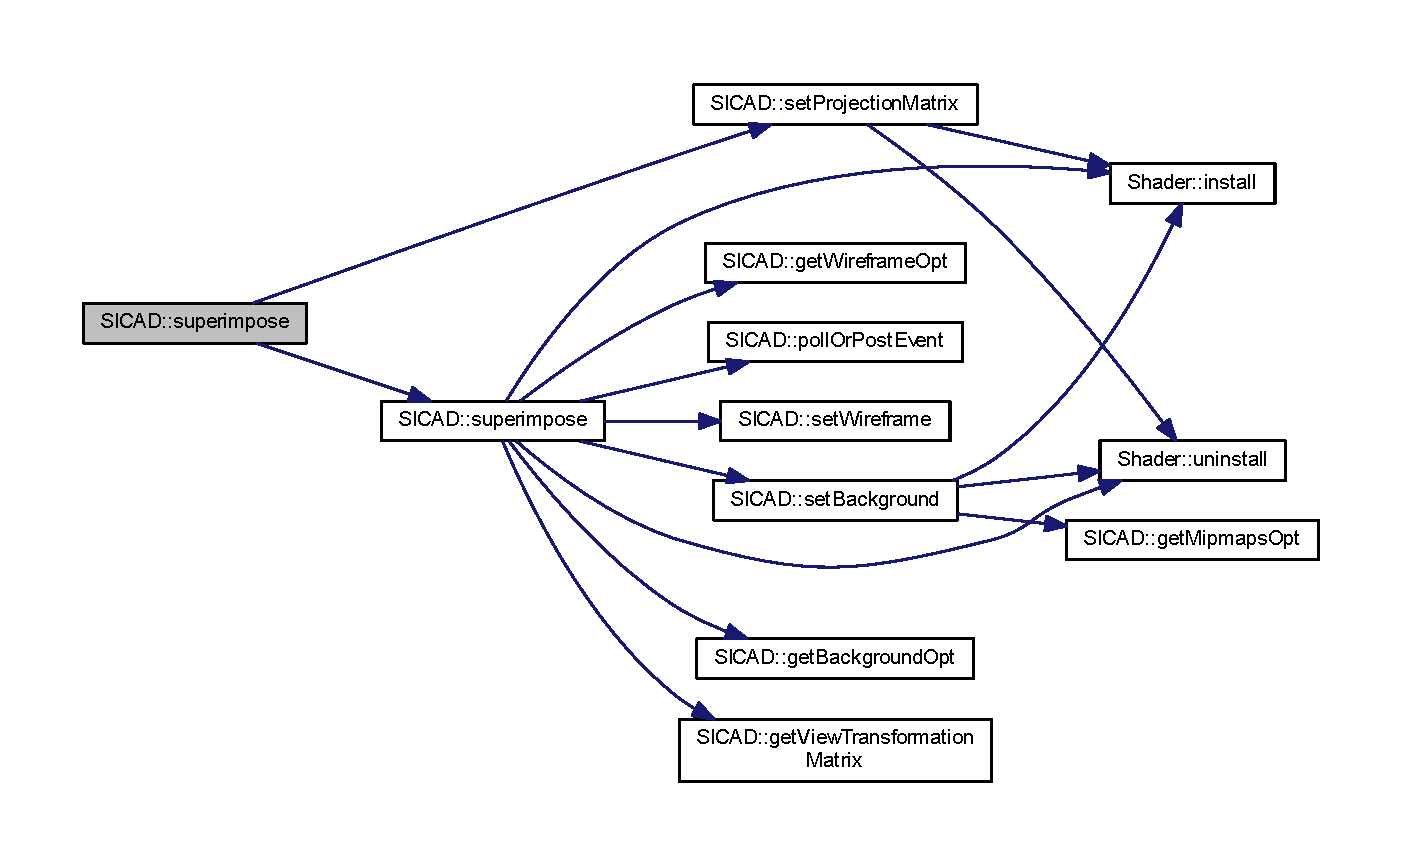
\includegraphics[width=350pt]{classSICAD_a269e238387393b44177daa4eae88fedd_cgraph}
\end{center}
\end{figure}


\subsection{Member Data Documentation}
\mbox{\Hypertarget{classSICAD_ad5945f84df0d90113a24b2001ecbc832}\label{classSICAD_ad5945f84df0d90113a24b2001ecbc832}} 
\index{S\+I\+C\+AD@{S\+I\+C\+AD}!back\+\_\+proj\+\_\+@{back\+\_\+proj\+\_\+}}
\index{back\+\_\+proj\+\_\+@{back\+\_\+proj\+\_\+}!S\+I\+C\+AD@{S\+I\+C\+AD}}
\subsubsection{\texorpdfstring{back\+\_\+proj\+\_\+}{back\_proj\_}}
{\footnotesize\ttfamily glm\+::mat4 S\+I\+C\+A\+D\+::back\+\_\+proj\+\_\+\hspace{0.3cm}{\ttfamily [private]}}



Definition at line 205 of file S\+I\+C\+A\+D.\+h.



Referenced by init\+S\+I\+C\+A\+D(), and set\+Background().

\mbox{\Hypertarget{classSICAD_a16f7c3c77ddea5ba57bbcbcdd7a8d125}\label{classSICAD_a16f7c3c77ddea5ba57bbcbcdd7a8d125}} 
\index{S\+I\+C\+AD@{S\+I\+C\+AD}!class\+\_\+counter\+\_\+@{class\+\_\+counter\+\_\+}}
\index{class\+\_\+counter\+\_\+@{class\+\_\+counter\+\_\+}!S\+I\+C\+AD@{S\+I\+C\+AD}}
\subsubsection{\texorpdfstring{class\+\_\+counter\+\_\+}{class\_counter\_}}
{\footnotesize\ttfamily int S\+I\+C\+A\+D\+::class\+\_\+counter\+\_\+ = 0\hspace{0.3cm}{\ttfamily [static]}, {\ttfamily [private]}}



Definition at line 167 of file S\+I\+C\+A\+D.\+h.



Referenced by init\+S\+I\+C\+A\+D(), and $\sim$\+S\+I\+C\+A\+D().

\mbox{\Hypertarget{classSICAD_a2cdcd11dd55a4b02b85d7c32435cc719}\label{classSICAD_a2cdcd11dd55a4b02b85d7c32435cc719}} 
\index{S\+I\+C\+AD@{S\+I\+C\+AD}!ebo\+\_\+background\+\_\+@{ebo\+\_\+background\+\_\+}}
\index{ebo\+\_\+background\+\_\+@{ebo\+\_\+background\+\_\+}!S\+I\+C\+AD@{S\+I\+C\+AD}}
\subsubsection{\texorpdfstring{ebo\+\_\+background\+\_\+}{ebo\_background\_}}
{\footnotesize\ttfamily G\+Luint S\+I\+C\+A\+D\+::ebo\+\_\+background\+\_\+\hspace{0.3cm}{\ttfamily [private]}}



Definition at line 201 of file S\+I\+C\+A\+D.\+h.



Referenced by init\+S\+I\+C\+A\+D(), and $\sim$\+S\+I\+C\+A\+D().

\mbox{\Hypertarget{classSICAD_a4c4d2e249ac824528e1fe9f97fa207d9}\label{classSICAD_a4c4d2e249ac824528e1fe9f97fa207d9}} 
\index{S\+I\+C\+AD@{S\+I\+C\+AD}!far\+\_\+@{far\+\_\+}}
\index{far\+\_\+@{far\+\_\+}!S\+I\+C\+AD@{S\+I\+C\+AD}}
\subsubsection{\texorpdfstring{far\+\_\+}{far\_}}
{\footnotesize\ttfamily const G\+Lfloat S\+I\+C\+A\+D\+::far\+\_\+ = 1000.\+0f\hspace{0.3cm}{\ttfamily [private]}}



Definition at line 185 of file S\+I\+C\+A\+D.\+h.



Referenced by init\+S\+I\+C\+A\+D(), and set\+Projection\+Matrix().

\mbox{\Hypertarget{classSICAD_a2c173ad18d42e090b46a539f92f3fe9d}\label{classSICAD_a2c173ad18d42e090b46a539f92f3fe9d}} 
\index{S\+I\+C\+AD@{S\+I\+C\+AD}!fbo\+\_\+@{fbo\+\_\+}}
\index{fbo\+\_\+@{fbo\+\_\+}!S\+I\+C\+AD@{S\+I\+C\+AD}}
\subsubsection{\texorpdfstring{fbo\+\_\+}{fbo\_}}
{\footnotesize\ttfamily G\+Luint S\+I\+C\+A\+D\+::fbo\+\_\+\hspace{0.3cm}{\ttfamily [private]}}



Definition at line 196 of file S\+I\+C\+A\+D.\+h.



Referenced by init\+S\+I\+C\+A\+D(), superimpose(), and $\sim$\+S\+I\+C\+A\+D().

\mbox{\Hypertarget{classSICAD_a3361bb03e52bc0554bb1e3670ef3a0f9}\label{classSICAD_a3361bb03e52bc0554bb1e3670ef3a0f9}} 
\index{S\+I\+C\+AD@{S\+I\+C\+AD}!framebuffer\+\_\+height\+\_\+@{framebuffer\+\_\+height\+\_\+}}
\index{framebuffer\+\_\+height\+\_\+@{framebuffer\+\_\+height\+\_\+}!S\+I\+C\+AD@{S\+I\+C\+AD}}
\subsubsection{\texorpdfstring{framebuffer\+\_\+height\+\_\+}{framebuffer\_height\_}}
{\footnotesize\ttfamily G\+Lsizei S\+I\+C\+A\+D\+::framebuffer\+\_\+height\+\_\+ = 0\hspace{0.3cm}{\ttfamily [private]}}



Definition at line 181 of file S\+I\+C\+A\+D.\+h.



Referenced by init\+O\+G\+L(), init\+S\+I\+C\+A\+D(), and superimpose().

\mbox{\Hypertarget{classSICAD_a08c86b826a1784b132bac3f0792fc604}\label{classSICAD_a08c86b826a1784b132bac3f0792fc604}} 
\index{S\+I\+C\+AD@{S\+I\+C\+AD}!framebuffer\+\_\+width\+\_\+@{framebuffer\+\_\+width\+\_\+}}
\index{framebuffer\+\_\+width\+\_\+@{framebuffer\+\_\+width\+\_\+}!S\+I\+C\+AD@{S\+I\+C\+AD}}
\subsubsection{\texorpdfstring{framebuffer\+\_\+width\+\_\+}{framebuffer\_width\_}}
{\footnotesize\ttfamily G\+Lsizei S\+I\+C\+A\+D\+::framebuffer\+\_\+width\+\_\+ = 0\hspace{0.3cm}{\ttfamily [private]}}



Definition at line 180 of file S\+I\+C\+A\+D.\+h.



Referenced by init\+O\+G\+L(), init\+S\+I\+C\+A\+D(), and superimpose().

\mbox{\Hypertarget{classSICAD_a0eb57d114f3f6b50be13bd882552b2f7}\label{classSICAD_a0eb57d114f3f6b50be13bd882552b2f7}} 
\index{S\+I\+C\+AD@{S\+I\+C\+AD}!has\+\_\+proj\+\_\+matrix\+\_\+@{has\+\_\+proj\+\_\+matrix\+\_\+}}
\index{has\+\_\+proj\+\_\+matrix\+\_\+@{has\+\_\+proj\+\_\+matrix\+\_\+}!S\+I\+C\+AD@{S\+I\+C\+AD}}
\subsubsection{\texorpdfstring{has\+\_\+proj\+\_\+matrix\+\_\+}{has\_proj\_matrix\_}}
{\footnotesize\ttfamily bool S\+I\+C\+A\+D\+::has\+\_\+proj\+\_\+matrix\+\_\+ = false\hspace{0.3cm}{\ttfamily [private]}}



Definition at line 164 of file S\+I\+C\+A\+D.\+h.



Referenced by set\+Projection\+Matrix(), and superimpose().

\mbox{\Hypertarget{classSICAD_a093da94bc84a46d08f71051c4d88c176}\label{classSICAD_a093da94bc84a46d08f71051c4d88c176}} 
\index{S\+I\+C\+AD@{S\+I\+C\+AD}!image\+\_\+height\+\_\+@{image\+\_\+height\+\_\+}}
\index{image\+\_\+height\+\_\+@{image\+\_\+height\+\_\+}!S\+I\+C\+AD@{S\+I\+C\+AD}}
\subsubsection{\texorpdfstring{image\+\_\+height\+\_\+}{image\_height\_}}
{\footnotesize\ttfamily G\+Lsizei S\+I\+C\+A\+D\+::image\+\_\+height\+\_\+ = 0\hspace{0.3cm}{\ttfamily [private]}}



Definition at line 178 of file S\+I\+C\+A\+D.\+h.



Referenced by init\+O\+G\+L().

\mbox{\Hypertarget{classSICAD_ade37d5c3960d164acaa749745f55070f}\label{classSICAD_ade37d5c3960d164acaa749745f55070f}} 
\index{S\+I\+C\+AD@{S\+I\+C\+AD}!image\+\_\+width\+\_\+@{image\+\_\+width\+\_\+}}
\index{image\+\_\+width\+\_\+@{image\+\_\+width\+\_\+}!S\+I\+C\+AD@{S\+I\+C\+AD}}
\subsubsection{\texorpdfstring{image\+\_\+width\+\_\+}{image\_width\_}}
{\footnotesize\ttfamily G\+Lsizei S\+I\+C\+A\+D\+::image\+\_\+width\+\_\+ = 0\hspace{0.3cm}{\ttfamily [private]}}



Definition at line 177 of file S\+I\+C\+A\+D.\+h.



Referenced by init\+O\+G\+L().

\mbox{\Hypertarget{classSICAD_aa624c978497506de4a255c5f0301579f}\label{classSICAD_aa624c978497506de4a255c5f0301579f}} 
\index{S\+I\+C\+AD@{S\+I\+C\+AD}!is\+\_\+initialized\+\_\+@{is\+\_\+initialized\+\_\+}}
\index{is\+\_\+initialized\+\_\+@{is\+\_\+initialized\+\_\+}!S\+I\+C\+AD@{S\+I\+C\+AD}}
\subsubsection{\texorpdfstring{is\+\_\+initialized\+\_\+}{is\_initialized\_}}
{\footnotesize\ttfamily bool S\+I\+C\+A\+D\+::is\+\_\+initialized\+\_\+ = false\hspace{0.3cm}{\ttfamily [private]}}



Definition at line 163 of file S\+I\+C\+A\+D.\+h.



Referenced by get\+Ogl\+Window\+Should\+Close(), init\+S\+I\+C\+A\+D(), set\+Ogl\+Window\+Should\+Close(), set\+Projection\+Matrix(), and superimpose().

\mbox{\Hypertarget{classSICAD_a9eb34b659cac13b8442ca821455cc1f1}\label{classSICAD_a9eb34b659cac13b8442ca821455cc1f1}} 
\index{S\+I\+C\+AD@{S\+I\+C\+AD}!log\+\_\+\+I\+D\+\_\+@{log\+\_\+\+I\+D\+\_\+}}
\index{log\+\_\+\+I\+D\+\_\+@{log\+\_\+\+I\+D\+\_\+}!S\+I\+C\+AD@{S\+I\+C\+AD}}
\subsubsection{\texorpdfstring{log\+\_\+\+I\+D\+\_\+}{log\_ID\_}}
{\footnotesize\ttfamily const std\+::string S\+I\+C\+A\+D\+::log\+\_\+\+I\+D\+\_\+ = \char`\"{}\mbox{[}SI-\/C\+AD\mbox{]}\char`\"{}\hspace{0.3cm}{\ttfamily [private]}}



Definition at line 171 of file S\+I\+C\+A\+D.\+h.



Referenced by init\+O\+G\+L(), init\+S\+I\+C\+A\+D(), S\+I\+C\+A\+D(), and $\sim$\+S\+I\+C\+A\+D().

\mbox{\Hypertarget{classSICAD_a6a4623d27b2ee48ad0db90bd075c708c}\label{classSICAD_a6a4623d27b2ee48ad0db90bd075c708c}} 
\index{S\+I\+C\+AD@{S\+I\+C\+AD}!main\+\_\+thread\+\_\+id\+\_\+@{main\+\_\+thread\+\_\+id\+\_\+}}
\index{main\+\_\+thread\+\_\+id\+\_\+@{main\+\_\+thread\+\_\+id\+\_\+}!S\+I\+C\+AD@{S\+I\+C\+AD}}
\subsubsection{\texorpdfstring{main\+\_\+thread\+\_\+id\+\_\+}{main\_thread\_id\_}}
{\footnotesize\ttfamily std\+::thread\+::id S\+I\+C\+A\+D\+::main\+\_\+thread\+\_\+id\+\_\+\hspace{0.3cm}{\ttfamily [private]}}



Definition at line 187 of file S\+I\+C\+A\+D.\+h.



Referenced by init\+O\+G\+L(), and poll\+Or\+Post\+Event().

\mbox{\Hypertarget{classSICAD_a34b0de96321855145937cc5858c019b0}\label{classSICAD_a34b0de96321855145937cc5858c019b0}} 
\index{S\+I\+C\+AD@{S\+I\+C\+AD}!mesh\+\_\+mmaps\+\_\+@{mesh\+\_\+mmaps\+\_\+}}
\index{mesh\+\_\+mmaps\+\_\+@{mesh\+\_\+mmaps\+\_\+}!S\+I\+C\+AD@{S\+I\+C\+AD}}
\subsubsection{\texorpdfstring{mesh\+\_\+mmaps\+\_\+}{mesh\_mmaps\_}}
{\footnotesize\ttfamily \mbox{\hyperlink{classSICAD_a7e092dede6f660355462d6d548214198}{M\+I\+P\+Maps}} S\+I\+C\+A\+D\+::mesh\+\_\+mmaps\+\_\+ = \mbox{\hyperlink{classSICAD_a7e092dede6f660355462d6d548214198ad879c351426770bc0b13c3628db1e636}{M\+I\+P\+Maps\+::nearest}}\hspace{0.3cm}{\ttfamily [private]}}



Definition at line 191 of file S\+I\+C\+A\+D.\+h.



Referenced by get\+Mipmaps\+Opt().

\mbox{\Hypertarget{classSICAD_a05fea2b5b027a3b7f37ef9ea4ecd64f0}\label{classSICAD_a05fea2b5b027a3b7f37ef9ea4ecd64f0}} 
\index{S\+I\+C\+AD@{S\+I\+C\+AD}!model\+\_\+obj\+\_\+@{model\+\_\+obj\+\_\+}}
\index{model\+\_\+obj\+\_\+@{model\+\_\+obj\+\_\+}!S\+I\+C\+AD@{S\+I\+C\+AD}}
\subsubsection{\texorpdfstring{model\+\_\+obj\+\_\+}{model\_obj\_}}
{\footnotesize\ttfamily \mbox{\hyperlink{classSICAD_aca3c9693d298f2e8dc171194c6a7507c}{Model\+Container}} S\+I\+C\+A\+D\+::model\+\_\+obj\+\_\+\hspace{0.3cm}{\ttfamily [private]}}



Definition at line 195 of file S\+I\+C\+A\+D.\+h.



Referenced by init\+S\+I\+C\+A\+D(), superimpose(), and $\sim$\+S\+I\+C\+A\+D().

\mbox{\Hypertarget{classSICAD_a690437655965101bad97d32e98015dd5}\label{classSICAD_a690437655965101bad97d32e98015dd5}} 
\index{S\+I\+C\+AD@{S\+I\+C\+AD}!near\+\_\+@{near\+\_\+}}
\index{near\+\_\+@{near\+\_\+}!S\+I\+C\+AD@{S\+I\+C\+AD}}
\subsubsection{\texorpdfstring{near\+\_\+}{near\_}}
{\footnotesize\ttfamily const G\+Lfloat S\+I\+C\+A\+D\+::near\+\_\+ = 0.\+001f\hspace{0.3cm}{\ttfamily [private]}}



Definition at line 184 of file S\+I\+C\+A\+D.\+h.



Referenced by set\+Projection\+Matrix().

\mbox{\Hypertarget{classSICAD_a95af2758122e6420369516fd13fd03cc}\label{classSICAD_a95af2758122e6420369516fd13fd03cc}} 
\index{S\+I\+C\+AD@{S\+I\+C\+AD}!ogl\+\_\+to\+\_\+cam\+\_\+@{ogl\+\_\+to\+\_\+cam\+\_\+}}
\index{ogl\+\_\+to\+\_\+cam\+\_\+@{ogl\+\_\+to\+\_\+cam\+\_\+}!S\+I\+C\+AD@{S\+I\+C\+AD}}
\subsubsection{\texorpdfstring{ogl\+\_\+to\+\_\+cam\+\_\+}{ogl\_to\_cam\_}}
{\footnotesize\ttfamily glm\+::mat3 S\+I\+C\+A\+D\+::ogl\+\_\+to\+\_\+cam\+\_\+ = glm\+::mat3(1.\+0f)\hspace{0.3cm}{\ttfamily [private]}}



Definition at line 179 of file S\+I\+C\+A\+D.\+h.



Referenced by get\+View\+Transformation\+Matrix(), and init\+S\+I\+C\+A\+D().

\mbox{\Hypertarget{classSICAD_afb91b682fd1f6629f163ab321869e7e0}\label{classSICAD_afb91b682fd1f6629f163ab321869e7e0}} 
\index{S\+I\+C\+AD@{S\+I\+C\+AD}!projection\+\_\+@{projection\+\_\+}}
\index{projection\+\_\+@{projection\+\_\+}!S\+I\+C\+AD@{S\+I\+C\+AD}}
\subsubsection{\texorpdfstring{projection\+\_\+}{projection\_}}
{\footnotesize\ttfamily glm\+::mat4 S\+I\+C\+A\+D\+::projection\+\_\+\hspace{0.3cm}{\ttfamily [private]}}



Definition at line 206 of file S\+I\+C\+A\+D.\+h.



Referenced by set\+Projection\+Matrix().

\mbox{\Hypertarget{classSICAD_a29691bc258b500253364c9688f7af655}\label{classSICAD_a29691bc258b500253364c9688f7af655}} 
\index{S\+I\+C\+AD@{S\+I\+C\+AD}!render\+\_\+img\+\_\+height\+\_\+@{render\+\_\+img\+\_\+height\+\_\+}}
\index{render\+\_\+img\+\_\+height\+\_\+@{render\+\_\+img\+\_\+height\+\_\+}!S\+I\+C\+AD@{S\+I\+C\+AD}}
\subsubsection{\texorpdfstring{render\+\_\+img\+\_\+height\+\_\+}{render\_img\_height\_}}
{\footnotesize\ttfamily G\+Lsizei S\+I\+C\+A\+D\+::render\+\_\+img\+\_\+height\+\_\+ = 0\hspace{0.3cm}{\ttfamily [private]}}



Definition at line 183 of file S\+I\+C\+A\+D.\+h.



Referenced by init\+O\+G\+L(), and superimpose().

\mbox{\Hypertarget{classSICAD_acbd2113a0cc446db6f59fdedd890aad9}\label{classSICAD_acbd2113a0cc446db6f59fdedd890aad9}} 
\index{S\+I\+C\+AD@{S\+I\+C\+AD}!render\+\_\+img\+\_\+width\+\_\+@{render\+\_\+img\+\_\+width\+\_\+}}
\index{render\+\_\+img\+\_\+width\+\_\+@{render\+\_\+img\+\_\+width\+\_\+}!S\+I\+C\+AD@{S\+I\+C\+AD}}
\subsubsection{\texorpdfstring{render\+\_\+img\+\_\+width\+\_\+}{render\_img\_width\_}}
{\footnotesize\ttfamily G\+Lsizei S\+I\+C\+A\+D\+::render\+\_\+img\+\_\+width\+\_\+ = 0\hspace{0.3cm}{\ttfamily [private]}}



Definition at line 182 of file S\+I\+C\+A\+D.\+h.



Referenced by init\+O\+G\+L(), and superimpose().

\mbox{\Hypertarget{classSICAD_aca24504d58ce97106dbc95925f36fca0}\label{classSICAD_aca24504d58ce97106dbc95925f36fca0}} 
\index{S\+I\+C\+AD@{S\+I\+C\+AD}!renderbuffer\+\_\+size\+\_\+@{renderbuffer\+\_\+size\+\_\+}}
\index{renderbuffer\+\_\+size\+\_\+@{renderbuffer\+\_\+size\+\_\+}!S\+I\+C\+AD@{S\+I\+C\+AD}}
\subsubsection{\texorpdfstring{renderbuffer\+\_\+size\+\_\+}{renderbuffer\_size\_}}
{\footnotesize\ttfamily G\+Lsizei S\+I\+C\+A\+D\+::renderbuffer\+\_\+size\+\_\+ = 0\hspace{0.3cm}{\ttfamily [static]}, {\ttfamily [private]}}



Definition at line 168 of file S\+I\+C\+A\+D.\+h.



Referenced by init\+O\+G\+L().

\mbox{\Hypertarget{classSICAD_a46edf33acc9f7ea3bd98c7ee6388ce9c}\label{classSICAD_a46edf33acc9f7ea3bd98c7ee6388ce9c}} 
\index{S\+I\+C\+AD@{S\+I\+C\+AD}!shader\+\_\+background\+\_\+@{shader\+\_\+background\+\_\+}}
\index{shader\+\_\+background\+\_\+@{shader\+\_\+background\+\_\+}!S\+I\+C\+AD@{S\+I\+C\+AD}}
\subsubsection{\texorpdfstring{shader\+\_\+background\+\_\+}{shader\_background\_}}
{\footnotesize\ttfamily \mbox{\hyperlink{classShader}{Shader}}$\ast$ S\+I\+C\+A\+D\+::shader\+\_\+background\+\_\+ = nullptr\hspace{0.3cm}{\ttfamily [private]}}



Definition at line 192 of file S\+I\+C\+A\+D.\+h.



Referenced by init\+S\+I\+C\+A\+D(), set\+Background(), and $\sim$\+S\+I\+C\+A\+D().

\mbox{\Hypertarget{classSICAD_a6c11f0e8dc8cbdd91748c230fc680833}\label{classSICAD_a6c11f0e8dc8cbdd91748c230fc680833}} 
\index{S\+I\+C\+AD@{S\+I\+C\+AD}!shader\+\_\+cad\+\_\+@{shader\+\_\+cad\+\_\+}}
\index{shader\+\_\+cad\+\_\+@{shader\+\_\+cad\+\_\+}!S\+I\+C\+AD@{S\+I\+C\+AD}}
\subsubsection{\texorpdfstring{shader\+\_\+cad\+\_\+}{shader\_cad\_}}
{\footnotesize\ttfamily \mbox{\hyperlink{classShader}{Shader}}$\ast$ S\+I\+C\+A\+D\+::shader\+\_\+cad\+\_\+ = nullptr\hspace{0.3cm}{\ttfamily [private]}}



Definition at line 193 of file S\+I\+C\+A\+D.\+h.



Referenced by init\+S\+I\+C\+A\+D(), set\+Projection\+Matrix(), superimpose(), and $\sim$\+S\+I\+C\+A\+D().

\mbox{\Hypertarget{classSICAD_ac921e60623f3797253bcbcdd445b903b}\label{classSICAD_ac921e60623f3797253bcbcdd445b903b}} 
\index{S\+I\+C\+AD@{S\+I\+C\+AD}!shader\+\_\+frame\+\_\+@{shader\+\_\+frame\+\_\+}}
\index{shader\+\_\+frame\+\_\+@{shader\+\_\+frame\+\_\+}!S\+I\+C\+AD@{S\+I\+C\+AD}}
\subsubsection{\texorpdfstring{shader\+\_\+frame\+\_\+}{shader\_frame\_}}
{\footnotesize\ttfamily \mbox{\hyperlink{classShader}{Shader}}$\ast$ S\+I\+C\+A\+D\+::shader\+\_\+frame\+\_\+ = nullptr\hspace{0.3cm}{\ttfamily [private]}}



Definition at line 194 of file S\+I\+C\+A\+D.\+h.



Referenced by init\+S\+I\+C\+A\+D(), set\+Projection\+Matrix(), and superimpose().

\mbox{\Hypertarget{classSICAD_a8db9e37d71a14883be4879e9ea4b6a02}\label{classSICAD_a8db9e37d71a14883be4879e9ea4b6a02}} 
\index{S\+I\+C\+AD@{S\+I\+C\+AD}!show\+\_\+background\+\_\+@{show\+\_\+background\+\_\+}}
\index{show\+\_\+background\+\_\+@{show\+\_\+background\+\_\+}!S\+I\+C\+AD@{S\+I\+C\+AD}}
\subsubsection{\texorpdfstring{show\+\_\+background\+\_\+}{show\_background\_}}
{\footnotesize\ttfamily bool S\+I\+C\+A\+D\+::show\+\_\+background\+\_\+ = false\hspace{0.3cm}{\ttfamily [private]}}



Definition at line 189 of file S\+I\+C\+A\+D.\+h.



Referenced by get\+Background\+Opt(), and set\+Background\+Opt().

\mbox{\Hypertarget{classSICAD_a9c4c3ba5d071f763ee1956fa31faa3f8}\label{classSICAD_a9c4c3ba5d071f763ee1956fa31faa3f8}} 
\index{S\+I\+C\+AD@{S\+I\+C\+AD}!show\+\_\+mesh\+\_\+mode\+\_\+@{show\+\_\+mesh\+\_\+mode\+\_\+}}
\index{show\+\_\+mesh\+\_\+mode\+\_\+@{show\+\_\+mesh\+\_\+mode\+\_\+}!S\+I\+C\+AD@{S\+I\+C\+AD}}
\subsubsection{\texorpdfstring{show\+\_\+mesh\+\_\+mode\+\_\+}{show\_mesh\_mode\_}}
{\footnotesize\ttfamily G\+Lenum S\+I\+C\+A\+D\+::show\+\_\+mesh\+\_\+mode\+\_\+ = G\+L\+\_\+\+F\+I\+LL\hspace{0.3cm}{\ttfamily [private]}}



Definition at line 190 of file S\+I\+C\+A\+D.\+h.



Referenced by get\+Wireframe\+Opt(), and set\+Wireframe\+Opt().

\mbox{\Hypertarget{classSICAD_a2728fb0fa0be11f0992bc81b4873da4f}\label{classSICAD_a2728fb0fa0be11f0992bc81b4873da4f}} 
\index{S\+I\+C\+AD@{S\+I\+C\+AD}!texture\+\_\+background\+\_\+@{texture\+\_\+background\+\_\+}}
\index{texture\+\_\+background\+\_\+@{texture\+\_\+background\+\_\+}!S\+I\+C\+AD@{S\+I\+C\+AD}}
\subsubsection{\texorpdfstring{texture\+\_\+background\+\_\+}{texture\_background\_}}
{\footnotesize\ttfamily G\+Luint S\+I\+C\+A\+D\+::texture\+\_\+background\+\_\+\hspace{0.3cm}{\ttfamily [private]}}



Definition at line 199 of file S\+I\+C\+A\+D.\+h.



Referenced by init\+S\+I\+C\+A\+D(), set\+Background(), and $\sim$\+S\+I\+C\+A\+D().

\mbox{\Hypertarget{classSICAD_a50f1ec3b2545ca40d58466735da80fc6}\label{classSICAD_a50f1ec3b2545ca40d58466735da80fc6}} 
\index{S\+I\+C\+AD@{S\+I\+C\+AD}!texture\+\_\+color\+\_\+buffer\+\_\+@{texture\+\_\+color\+\_\+buffer\+\_\+}}
\index{texture\+\_\+color\+\_\+buffer\+\_\+@{texture\+\_\+color\+\_\+buffer\+\_\+}!S\+I\+C\+AD@{S\+I\+C\+AD}}
\subsubsection{\texorpdfstring{texture\+\_\+color\+\_\+buffer\+\_\+}{texture\_color\_buffer\_}}
{\footnotesize\ttfamily G\+Luint S\+I\+C\+A\+D\+::texture\+\_\+color\+\_\+buffer\+\_\+\hspace{0.3cm}{\ttfamily [private]}}



Definition at line 197 of file S\+I\+C\+A\+D.\+h.



Referenced by init\+S\+I\+C\+A\+D(), and $\sim$\+S\+I\+C\+A\+D().

\mbox{\Hypertarget{classSICAD_a2fed5ac56bb2206fe8f6eccc9d784015}\label{classSICAD_a2fed5ac56bb2206fe8f6eccc9d784015}} 
\index{S\+I\+C\+AD@{S\+I\+C\+AD}!texture\+\_\+depth\+\_\+buffer\+\_\+@{texture\+\_\+depth\+\_\+buffer\+\_\+}}
\index{texture\+\_\+depth\+\_\+buffer\+\_\+@{texture\+\_\+depth\+\_\+buffer\+\_\+}!S\+I\+C\+AD@{S\+I\+C\+AD}}
\subsubsection{\texorpdfstring{texture\+\_\+depth\+\_\+buffer\+\_\+}{texture\_depth\_buffer\_}}
{\footnotesize\ttfamily G\+Luint S\+I\+C\+A\+D\+::texture\+\_\+depth\+\_\+buffer\+\_\+\hspace{0.3cm}{\ttfamily [private]}}



Definition at line 198 of file S\+I\+C\+A\+D.\+h.



Referenced by init\+S\+I\+C\+A\+D(), and $\sim$\+S\+I\+C\+A\+D().

\mbox{\Hypertarget{classSICAD_ac2678cc1ad1b008912fec7e6892b23e1}\label{classSICAD_ac2678cc1ad1b008912fec7e6892b23e1}} 
\index{S\+I\+C\+AD@{S\+I\+C\+AD}!tiles\+\_\+cols\+\_\+@{tiles\+\_\+cols\+\_\+}}
\index{tiles\+\_\+cols\+\_\+@{tiles\+\_\+cols\+\_\+}!S\+I\+C\+AD@{S\+I\+C\+AD}}
\subsubsection{\texorpdfstring{tiles\+\_\+cols\+\_\+}{tiles\_cols\_}}
{\footnotesize\ttfamily G\+Lsizei S\+I\+C\+A\+D\+::tiles\+\_\+cols\+\_\+ = 0\hspace{0.3cm}{\ttfamily [private]}}



Definition at line 175 of file S\+I\+C\+A\+D.\+h.



Referenced by get\+Tiles\+Cols(), get\+Tiles\+Number(), init\+O\+G\+L(), and superimpose().

\mbox{\Hypertarget{classSICAD_a68723ee57cc9a1e02bc0dbda54a584ff}\label{classSICAD_a68723ee57cc9a1e02bc0dbda54a584ff}} 
\index{S\+I\+C\+AD@{S\+I\+C\+AD}!tiles\+\_\+num\+\_\+@{tiles\+\_\+num\+\_\+}}
\index{tiles\+\_\+num\+\_\+@{tiles\+\_\+num\+\_\+}!S\+I\+C\+AD@{S\+I\+C\+AD}}
\subsubsection{\texorpdfstring{tiles\+\_\+num\+\_\+}{tiles\_num\_}}
{\footnotesize\ttfamily G\+Lint S\+I\+C\+A\+D\+::tiles\+\_\+num\+\_\+ = 0\hspace{0.3cm}{\ttfamily [private]}}



Definition at line 174 of file S\+I\+C\+A\+D.\+h.



Referenced by init\+O\+G\+L(), and superimpose().

\mbox{\Hypertarget{classSICAD_aca3efa8f3fb75b3ee02474d4ec00e49e}\label{classSICAD_aca3efa8f3fb75b3ee02474d4ec00e49e}} 
\index{S\+I\+C\+AD@{S\+I\+C\+AD}!tiles\+\_\+rows\+\_\+@{tiles\+\_\+rows\+\_\+}}
\index{tiles\+\_\+rows\+\_\+@{tiles\+\_\+rows\+\_\+}!S\+I\+C\+AD@{S\+I\+C\+AD}}
\subsubsection{\texorpdfstring{tiles\+\_\+rows\+\_\+}{tiles\_rows\_}}
{\footnotesize\ttfamily G\+Lsizei S\+I\+C\+A\+D\+::tiles\+\_\+rows\+\_\+ = 0\hspace{0.3cm}{\ttfamily [private]}}



Definition at line 176 of file S\+I\+C\+A\+D.\+h.



Referenced by get\+Tiles\+Number(), get\+Tiles\+Rows(), init\+O\+G\+L(), and superimpose().

\mbox{\Hypertarget{classSICAD_a19306fe768bae547e18a3b9366e37389}\label{classSICAD_a19306fe768bae547e18a3b9366e37389}} 
\index{S\+I\+C\+AD@{S\+I\+C\+AD}!vao\+\_\+background\+\_\+@{vao\+\_\+background\+\_\+}}
\index{vao\+\_\+background\+\_\+@{vao\+\_\+background\+\_\+}!S\+I\+C\+AD@{S\+I\+C\+AD}}
\subsubsection{\texorpdfstring{vao\+\_\+background\+\_\+}{vao\_background\_}}
{\footnotesize\ttfamily G\+Luint S\+I\+C\+A\+D\+::vao\+\_\+background\+\_\+\hspace{0.3cm}{\ttfamily [private]}}



Definition at line 200 of file S\+I\+C\+A\+D.\+h.



Referenced by init\+S\+I\+C\+A\+D(), set\+Background(), and $\sim$\+S\+I\+C\+A\+D().

\mbox{\Hypertarget{classSICAD_ae91abeb0fe30f27e0fc40649235f3437}\label{classSICAD_ae91abeb0fe30f27e0fc40649235f3437}} 
\index{S\+I\+C\+AD@{S\+I\+C\+AD}!vao\+\_\+frame\+\_\+@{vao\+\_\+frame\+\_\+}}
\index{vao\+\_\+frame\+\_\+@{vao\+\_\+frame\+\_\+}!S\+I\+C\+AD@{S\+I\+C\+AD}}
\subsubsection{\texorpdfstring{vao\+\_\+frame\+\_\+}{vao\_frame\_}}
{\footnotesize\ttfamily G\+Luint S\+I\+C\+A\+D\+::vao\+\_\+frame\+\_\+\hspace{0.3cm}{\ttfamily [private]}}



Definition at line 203 of file S\+I\+C\+A\+D.\+h.



Referenced by init\+S\+I\+C\+A\+D(), superimpose(), and $\sim$\+S\+I\+C\+A\+D().

\mbox{\Hypertarget{classSICAD_a86d6184b8c557460317a158e8d9508d1}\label{classSICAD_a86d6184b8c557460317a158e8d9508d1}} 
\index{S\+I\+C\+AD@{S\+I\+C\+AD}!vbo\+\_\+background\+\_\+@{vbo\+\_\+background\+\_\+}}
\index{vbo\+\_\+background\+\_\+@{vbo\+\_\+background\+\_\+}!S\+I\+C\+AD@{S\+I\+C\+AD}}
\subsubsection{\texorpdfstring{vbo\+\_\+background\+\_\+}{vbo\_background\_}}
{\footnotesize\ttfamily G\+Luint S\+I\+C\+A\+D\+::vbo\+\_\+background\+\_\+\hspace{0.3cm}{\ttfamily [private]}}



Definition at line 202 of file S\+I\+C\+A\+D.\+h.



Referenced by init\+S\+I\+C\+A\+D(), and $\sim$\+S\+I\+C\+A\+D().

\mbox{\Hypertarget{classSICAD_af58ffe3edf622ab96f669fcd6e210be9}\label{classSICAD_af58ffe3edf622ab96f669fcd6e210be9}} 
\index{S\+I\+C\+AD@{S\+I\+C\+AD}!vbo\+\_\+frame\+\_\+@{vbo\+\_\+frame\+\_\+}}
\index{vbo\+\_\+frame\+\_\+@{vbo\+\_\+frame\+\_\+}!S\+I\+C\+AD@{S\+I\+C\+AD}}
\subsubsection{\texorpdfstring{vbo\+\_\+frame\+\_\+}{vbo\_frame\_}}
{\footnotesize\ttfamily G\+Luint S\+I\+C\+A\+D\+::vbo\+\_\+frame\+\_\+\hspace{0.3cm}{\ttfamily [private]}}



Definition at line 204 of file S\+I\+C\+A\+D.\+h.



Referenced by init\+S\+I\+C\+A\+D(), and $\sim$\+S\+I\+C\+A\+D().

\mbox{\Hypertarget{classSICAD_a3e55fa9ffa99ef200bfc15d6a105698a}\label{classSICAD_a3e55fa9ffa99ef200bfc15d6a105698a}} 
\index{S\+I\+C\+AD@{S\+I\+C\+AD}!window\+\_\+@{window\+\_\+}}
\index{window\+\_\+@{window\+\_\+}!S\+I\+C\+AD@{S\+I\+C\+AD}}
\subsubsection{\texorpdfstring{window\+\_\+}{window\_}}
{\footnotesize\ttfamily G\+L\+F\+Wwindow$\ast$ S\+I\+C\+A\+D\+::window\+\_\+ = nullptr\hspace{0.3cm}{\ttfamily [private]}}



Definition at line 173 of file S\+I\+C\+A\+D.\+h.



Referenced by get\+Ogl\+Window\+Should\+Close(), init\+O\+G\+L(), init\+S\+I\+C\+A\+D(), set\+Ogl\+Window\+Should\+Close(), set\+Projection\+Matrix(), superimpose(), and $\sim$\+S\+I\+C\+A\+D().



The documentation for this class was generated from the following files\+:\begin{DoxyCompactItemize}
\item 
C\+:/\+Users/cfantacci/\+Git\+Hub/superimpose-\/mesh-\/lib/src/\+Superimpose\+Mesh/include/\+Superimpose\+Mesh/\mbox{\hyperlink{SICAD_8h}{S\+I\+C\+A\+D.\+h}}\item 
C\+:/\+Users/cfantacci/\+Git\+Hub/superimpose-\/mesh-\/lib/src/\+Superimpose\+Mesh/src/\mbox{\hyperlink{SICAD_8cpp}{S\+I\+C\+A\+D.\+cpp}}\end{DoxyCompactItemize}

\hypertarget{classSISkeleton}{}\section{S\+I\+Skeleton Class Reference}
\label{classSISkeleton}\index{S\+I\+Skeleton@{S\+I\+Skeleton}}


{\ttfamily \#include $<$S\+I\+Skeleton.\+h$>$}



Inheritance diagram for S\+I\+Skeleton\+:
\nopagebreak
\begin{figure}[H]
\begin{center}
\leavevmode
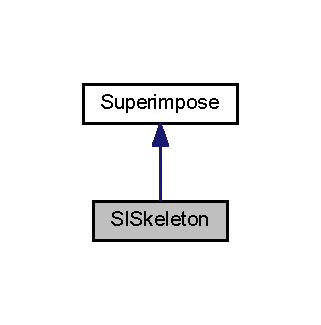
\includegraphics[width=154pt]{classSISkeleton__inherit__graph}
\end{center}
\end{figure}
\subsection*{Public Types}
\begin{DoxyCompactItemize}
\item 
typedef std\+::vector$<$ double $>$ \mbox{\hyperlink{classSuperimpose_a85d40a5caf19f486d1e0c15c0a025378}{Model\+Pose}}
\item 
typedef std\+::multimap$<$ std\+::string, \mbox{\hyperlink{classSuperimpose_a85d40a5caf19f486d1e0c15c0a025378}{Model\+Pose}} $>$ \mbox{\hyperlink{classSuperimpose_a178e3d4e2def6635bfcf9454dd4b5d22}{Model\+Pose\+Container}}
\item 
typedef std\+::pair$<$ std\+::string, \mbox{\hyperlink{classSuperimpose_a85d40a5caf19f486d1e0c15c0a025378}{Model\+Pose}} $>$ \mbox{\hyperlink{classSuperimpose_a1e02e0225687b42296dcfee4eadf8a55}{Model\+Pose\+Container\+Element}}
\end{DoxyCompactItemize}
\subsection*{Public Member Functions}
\begin{DoxyCompactItemize}
\item 
\mbox{\hyperlink{classSISkeleton_a52ad426ff55dacaea6fb30470a7e67ff}{S\+I\+Skeleton}} ()
\item 
\mbox{\hyperlink{classSISkeleton_a3d968efd0700f20a93064957f15bf40e}{S\+I\+Skeleton}} (const float cam\+\_\+fx, const float cam\+\_\+fy, const float cam\+\_\+cx, const float cam\+\_\+cy)
\item 
\mbox{\hyperlink{classSISkeleton_a6e9f780999700a4695d4ed487f2499b9}{$\sim$\+S\+I\+Skeleton}} ()
\item 
bool \mbox{\hyperlink{classSISkeleton_a3f49fa3419370c2597435768f280c747}{superimpose}} (const \mbox{\hyperlink{classSuperimpose_a178e3d4e2def6635bfcf9454dd4b5d22}{Model\+Pose\+Container}} \&objpos\+\_\+map, const double $\ast$cam\+\_\+x, const double $\ast$cam\+\_\+o, cv\+::\+Mat \&img) override
\item 
bool \mbox{\hyperlink{classSISkeleton_aa1f5e1a67363038821a5d514fb361a38}{set\+Projection\+Matrix}} (const float cam\+\_\+fx, const float cam\+\_\+fy, const float cam\+\_\+cx, const float cam\+\_\+cy)
\end{DoxyCompactItemize}
\subsection*{Protected Member Functions}
\begin{DoxyCompactItemize}
\item 
glm\+::vec2 \mbox{\hyperlink{classSISkeleton_adbd224633ac2e4c0285cf2cf760cc42a}{get\+World\+To\+Pixel}} (const double $\ast$world\+\_\+point)
\end{DoxyCompactItemize}
\subsection*{Private Attributes}
\begin{DoxyCompactItemize}
\item 
const std\+::string \mbox{\hyperlink{classSISkeleton_a6d4a9061880520792f467eb8e7faa66b}{log\+\_\+\+I\+D\+\_\+}} = \char`\"{}\mbox{[}SI-\/Skeleton\mbox{]}\char`\"{}
\item 
std\+::list$<$ std\+::string $>$ \mbox{\hyperlink{classSISkeleton_ae88bbaec338923a85f4afbf8704a6933}{hand\+\_\+part\+\_\+}}
\item 
glm\+::mat3 \mbox{\hyperlink{classSISkeleton_a1ac569493d56bf099bdc364318ad5622}{projection\+\_\+}}
\item 
glm\+::mat3 \mbox{\hyperlink{classSISkeleton_a476442a8c9e9a1f4a703c3a84f0b83f1}{root\+\_\+to\+\_\+eye\+\_\+}}
\item 
glm\+::vec3 \mbox{\hyperlink{classSISkeleton_a63f1395d3e57e2d6a6d7de50928221a2}{cam\+\_\+pos\+\_\+}}
\end{DoxyCompactItemize}


\subsection{Detailed Description}


Definition at line 12 of file S\+I\+Skeleton.\+h.



\subsection{Member Typedef Documentation}
\mbox{\Hypertarget{classSuperimpose_a85d40a5caf19f486d1e0c15c0a025378}\label{classSuperimpose_a85d40a5caf19f486d1e0c15c0a025378}} 
\index{S\+I\+Skeleton@{S\+I\+Skeleton}!Model\+Pose@{Model\+Pose}}
\index{Model\+Pose@{Model\+Pose}!S\+I\+Skeleton@{S\+I\+Skeleton}}
\subsubsection{\texorpdfstring{Model\+Pose}{ModelPose}}
{\footnotesize\ttfamily typedef std\+::vector$<$double$>$ \mbox{\hyperlink{classSuperimpose_a85d40a5caf19f486d1e0c15c0a025378}{Superimpose\+::\+Model\+Pose}}\hspace{0.3cm}{\ttfamily [inherited]}}



Definition at line 16 of file Superimpose.\+h.

\mbox{\Hypertarget{classSuperimpose_a178e3d4e2def6635bfcf9454dd4b5d22}\label{classSuperimpose_a178e3d4e2def6635bfcf9454dd4b5d22}} 
\index{S\+I\+Skeleton@{S\+I\+Skeleton}!Model\+Pose\+Container@{Model\+Pose\+Container}}
\index{Model\+Pose\+Container@{Model\+Pose\+Container}!S\+I\+Skeleton@{S\+I\+Skeleton}}
\subsubsection{\texorpdfstring{Model\+Pose\+Container}{ModelPoseContainer}}
{\footnotesize\ttfamily typedef std\+::multimap$<$std\+::string, \mbox{\hyperlink{classSuperimpose_a85d40a5caf19f486d1e0c15c0a025378}{Model\+Pose}}$>$ \mbox{\hyperlink{classSuperimpose_a178e3d4e2def6635bfcf9454dd4b5d22}{Superimpose\+::\+Model\+Pose\+Container}}\hspace{0.3cm}{\ttfamily [inherited]}}



Definition at line 17 of file Superimpose.\+h.

\mbox{\Hypertarget{classSuperimpose_a1e02e0225687b42296dcfee4eadf8a55}\label{classSuperimpose_a1e02e0225687b42296dcfee4eadf8a55}} 
\index{S\+I\+Skeleton@{S\+I\+Skeleton}!Model\+Pose\+Container\+Element@{Model\+Pose\+Container\+Element}}
\index{Model\+Pose\+Container\+Element@{Model\+Pose\+Container\+Element}!S\+I\+Skeleton@{S\+I\+Skeleton}}
\subsubsection{\texorpdfstring{Model\+Pose\+Container\+Element}{ModelPoseContainerElement}}
{\footnotesize\ttfamily typedef std\+::pair$<$std\+::string, \mbox{\hyperlink{classSuperimpose_a85d40a5caf19f486d1e0c15c0a025378}{Model\+Pose}}$>$ \mbox{\hyperlink{classSuperimpose_a1e02e0225687b42296dcfee4eadf8a55}{Superimpose\+::\+Model\+Pose\+Container\+Element}}\hspace{0.3cm}{\ttfamily [inherited]}}



Definition at line 18 of file Superimpose.\+h.



\subsection{Constructor \& Destructor Documentation}
\mbox{\Hypertarget{classSISkeleton_a52ad426ff55dacaea6fb30470a7e67ff}\label{classSISkeleton_a52ad426ff55dacaea6fb30470a7e67ff}} 
\index{S\+I\+Skeleton@{S\+I\+Skeleton}!S\+I\+Skeleton@{S\+I\+Skeleton}}
\index{S\+I\+Skeleton@{S\+I\+Skeleton}!S\+I\+Skeleton@{S\+I\+Skeleton}}
\subsubsection{\texorpdfstring{S\+I\+Skeleton()}{SISkeleton()}\hspace{0.1cm}{\footnotesize\ttfamily [1/2]}}
{\footnotesize\ttfamily S\+I\+Skeleton\+::\+S\+I\+Skeleton (\begin{DoxyParamCaption}{ }\end{DoxyParamCaption})}



Definition at line 11 of file S\+I\+Skeleton.\+cpp.

\mbox{\Hypertarget{classSISkeleton_a3d968efd0700f20a93064957f15bf40e}\label{classSISkeleton_a3d968efd0700f20a93064957f15bf40e}} 
\index{S\+I\+Skeleton@{S\+I\+Skeleton}!S\+I\+Skeleton@{S\+I\+Skeleton}}
\index{S\+I\+Skeleton@{S\+I\+Skeleton}!S\+I\+Skeleton@{S\+I\+Skeleton}}
\subsubsection{\texorpdfstring{S\+I\+Skeleton()}{SISkeleton()}\hspace{0.1cm}{\footnotesize\ttfamily [2/2]}}
{\footnotesize\ttfamily S\+I\+Skeleton\+::\+S\+I\+Skeleton (\begin{DoxyParamCaption}\item[{const float}]{cam\+\_\+fx,  }\item[{const float}]{cam\+\_\+fy,  }\item[{const float}]{cam\+\_\+cx,  }\item[{const float}]{cam\+\_\+cy }\end{DoxyParamCaption})}



Definition at line 17 of file S\+I\+Skeleton.\+cpp.



References log\+\_\+\+I\+D\+\_\+, and set\+Projection\+Matrix().

Here is the call graph for this function\+:
\nopagebreak
\begin{figure}[H]
\begin{center}
\leavevmode
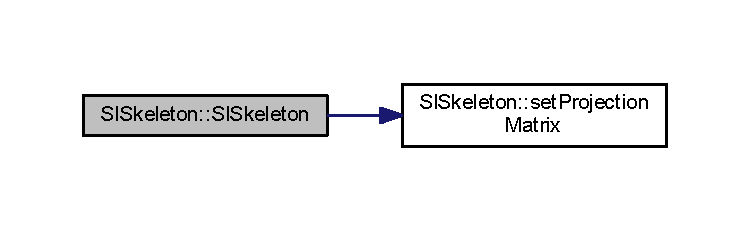
\includegraphics[width=350pt]{classSISkeleton_a3d968efd0700f20a93064957f15bf40e_cgraph}
\end{center}
\end{figure}
\mbox{\Hypertarget{classSISkeleton_a6e9f780999700a4695d4ed487f2499b9}\label{classSISkeleton_a6e9f780999700a4695d4ed487f2499b9}} 
\index{S\+I\+Skeleton@{S\+I\+Skeleton}!````~S\+I\+Skeleton@{$\sim$\+S\+I\+Skeleton}}
\index{````~S\+I\+Skeleton@{$\sim$\+S\+I\+Skeleton}!S\+I\+Skeleton@{S\+I\+Skeleton}}
\subsubsection{\texorpdfstring{$\sim$\+S\+I\+Skeleton()}{~SISkeleton()}}
{\footnotesize\ttfamily S\+I\+Skeleton\+::$\sim$\+S\+I\+Skeleton (\begin{DoxyParamCaption}{ }\end{DoxyParamCaption})}



Definition at line 26 of file S\+I\+Skeleton.\+cpp.



\subsection{Member Function Documentation}
\mbox{\Hypertarget{classSISkeleton_adbd224633ac2e4c0285cf2cf760cc42a}\label{classSISkeleton_adbd224633ac2e4c0285cf2cf760cc42a}} 
\index{S\+I\+Skeleton@{S\+I\+Skeleton}!get\+World\+To\+Pixel@{get\+World\+To\+Pixel}}
\index{get\+World\+To\+Pixel@{get\+World\+To\+Pixel}!S\+I\+Skeleton@{S\+I\+Skeleton}}
\subsubsection{\texorpdfstring{get\+World\+To\+Pixel()}{getWorldToPixel()}}
{\footnotesize\ttfamily glm\+::vec2 S\+I\+Skeleton\+::get\+World\+To\+Pixel (\begin{DoxyParamCaption}\item[{const double $\ast$}]{world\+\_\+point }\end{DoxyParamCaption})\hspace{0.3cm}{\ttfamily [protected]}}



Definition at line 76 of file S\+I\+Skeleton.\+cpp.



References cam\+\_\+pos\+\_\+, projection\+\_\+, and root\+\_\+to\+\_\+eye\+\_\+.



Referenced by superimpose().

\mbox{\Hypertarget{classSISkeleton_aa1f5e1a67363038821a5d514fb361a38}\label{classSISkeleton_aa1f5e1a67363038821a5d514fb361a38}} 
\index{S\+I\+Skeleton@{S\+I\+Skeleton}!set\+Projection\+Matrix@{set\+Projection\+Matrix}}
\index{set\+Projection\+Matrix@{set\+Projection\+Matrix}!S\+I\+Skeleton@{S\+I\+Skeleton}}
\subsubsection{\texorpdfstring{set\+Projection\+Matrix()}{setProjectionMatrix()}}
{\footnotesize\ttfamily bool S\+I\+Skeleton\+::set\+Projection\+Matrix (\begin{DoxyParamCaption}\item[{const float}]{cam\+\_\+fx,  }\item[{const float}]{cam\+\_\+fy,  }\item[{const float}]{cam\+\_\+cx,  }\item[{const float}]{cam\+\_\+cy }\end{DoxyParamCaption})}



Definition at line 60 of file S\+I\+Skeleton.\+cpp.



References projection\+\_\+.



Referenced by S\+I\+Skeleton().

\mbox{\Hypertarget{classSISkeleton_a3f49fa3419370c2597435768f280c747}\label{classSISkeleton_a3f49fa3419370c2597435768f280c747}} 
\index{S\+I\+Skeleton@{S\+I\+Skeleton}!superimpose@{superimpose}}
\index{superimpose@{superimpose}!S\+I\+Skeleton@{S\+I\+Skeleton}}
\subsubsection{\texorpdfstring{superimpose()}{superimpose()}}
{\footnotesize\ttfamily bool S\+I\+Skeleton\+::superimpose (\begin{DoxyParamCaption}\item[{const \mbox{\hyperlink{classSuperimpose_a178e3d4e2def6635bfcf9454dd4b5d22}{Model\+Pose\+Container}} \&}]{objpos\+\_\+map,  }\item[{const double $\ast$}]{cam\+\_\+x,  }\item[{const double $\ast$}]{cam\+\_\+o,  }\item[{cv\+::\+Mat \&}]{img }\end{DoxyParamCaption})\hspace{0.3cm}{\ttfamily [override]}, {\ttfamily [virtual]}}



Implements \mbox{\hyperlink{classSuperimpose_a62c4c269b8fc34cc36d3d54fa4acb35c}{Superimpose}}.



Definition at line 30 of file S\+I\+Skeleton.\+cpp.



References cam\+\_\+pos\+\_\+, get\+World\+To\+Pixel(), hand\+\_\+part\+\_\+, and root\+\_\+to\+\_\+eye\+\_\+.

Here is the call graph for this function\+:
\nopagebreak
\begin{figure}[H]
\begin{center}
\leavevmode
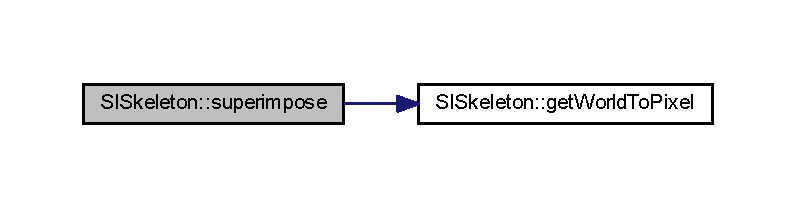
\includegraphics[width=350pt]{classSISkeleton_a3f49fa3419370c2597435768f280c747_cgraph}
\end{center}
\end{figure}


\subsection{Member Data Documentation}
\mbox{\Hypertarget{classSISkeleton_a63f1395d3e57e2d6a6d7de50928221a2}\label{classSISkeleton_a63f1395d3e57e2d6a6d7de50928221a2}} 
\index{S\+I\+Skeleton@{S\+I\+Skeleton}!cam\+\_\+pos\+\_\+@{cam\+\_\+pos\+\_\+}}
\index{cam\+\_\+pos\+\_\+@{cam\+\_\+pos\+\_\+}!S\+I\+Skeleton@{S\+I\+Skeleton}}
\subsubsection{\texorpdfstring{cam\+\_\+pos\+\_\+}{cam\_pos\_}}
{\footnotesize\ttfamily glm\+::vec3 S\+I\+Skeleton\+::cam\+\_\+pos\+\_\+\hspace{0.3cm}{\ttfamily [private]}}



Definition at line 34 of file S\+I\+Skeleton.\+h.



Referenced by get\+World\+To\+Pixel(), and superimpose().

\mbox{\Hypertarget{classSISkeleton_ae88bbaec338923a85f4afbf8704a6933}\label{classSISkeleton_ae88bbaec338923a85f4afbf8704a6933}} 
\index{S\+I\+Skeleton@{S\+I\+Skeleton}!hand\+\_\+part\+\_\+@{hand\+\_\+part\+\_\+}}
\index{hand\+\_\+part\+\_\+@{hand\+\_\+part\+\_\+}!S\+I\+Skeleton@{S\+I\+Skeleton}}
\subsubsection{\texorpdfstring{hand\+\_\+part\+\_\+}{hand\_part\_}}
{\footnotesize\ttfamily std\+::list$<$std\+::string$>$ S\+I\+Skeleton\+::hand\+\_\+part\+\_\+\hspace{0.3cm}{\ttfamily [private]}}



Definition at line 31 of file S\+I\+Skeleton.\+h.



Referenced by superimpose().

\mbox{\Hypertarget{classSISkeleton_a6d4a9061880520792f467eb8e7faa66b}\label{classSISkeleton_a6d4a9061880520792f467eb8e7faa66b}} 
\index{S\+I\+Skeleton@{S\+I\+Skeleton}!log\+\_\+\+I\+D\+\_\+@{log\+\_\+\+I\+D\+\_\+}}
\index{log\+\_\+\+I\+D\+\_\+@{log\+\_\+\+I\+D\+\_\+}!S\+I\+Skeleton@{S\+I\+Skeleton}}
\subsubsection{\texorpdfstring{log\+\_\+\+I\+D\+\_\+}{log\_ID\_}}
{\footnotesize\ttfamily const std\+::string S\+I\+Skeleton\+::log\+\_\+\+I\+D\+\_\+ = \char`\"{}\mbox{[}SI-\/Skeleton\mbox{]}\char`\"{}\hspace{0.3cm}{\ttfamily [private]}}



Definition at line 29 of file S\+I\+Skeleton.\+h.



Referenced by S\+I\+Skeleton().

\mbox{\Hypertarget{classSISkeleton_a1ac569493d56bf099bdc364318ad5622}\label{classSISkeleton_a1ac569493d56bf099bdc364318ad5622}} 
\index{S\+I\+Skeleton@{S\+I\+Skeleton}!projection\+\_\+@{projection\+\_\+}}
\index{projection\+\_\+@{projection\+\_\+}!S\+I\+Skeleton@{S\+I\+Skeleton}}
\subsubsection{\texorpdfstring{projection\+\_\+}{projection\_}}
{\footnotesize\ttfamily glm\+::mat3 S\+I\+Skeleton\+::projection\+\_\+\hspace{0.3cm}{\ttfamily [private]}}



Definition at line 32 of file S\+I\+Skeleton.\+h.



Referenced by get\+World\+To\+Pixel(), and set\+Projection\+Matrix().

\mbox{\Hypertarget{classSISkeleton_a476442a8c9e9a1f4a703c3a84f0b83f1}\label{classSISkeleton_a476442a8c9e9a1f4a703c3a84f0b83f1}} 
\index{S\+I\+Skeleton@{S\+I\+Skeleton}!root\+\_\+to\+\_\+eye\+\_\+@{root\+\_\+to\+\_\+eye\+\_\+}}
\index{root\+\_\+to\+\_\+eye\+\_\+@{root\+\_\+to\+\_\+eye\+\_\+}!S\+I\+Skeleton@{S\+I\+Skeleton}}
\subsubsection{\texorpdfstring{root\+\_\+to\+\_\+eye\+\_\+}{root\_to\_eye\_}}
{\footnotesize\ttfamily glm\+::mat3 S\+I\+Skeleton\+::root\+\_\+to\+\_\+eye\+\_\+\hspace{0.3cm}{\ttfamily [private]}}



Definition at line 33 of file S\+I\+Skeleton.\+h.



Referenced by get\+World\+To\+Pixel(), and superimpose().



The documentation for this class was generated from the following files\+:\begin{DoxyCompactItemize}
\item 
C\+:/\+Users/cfantacci/\+Git\+Hub/superimpose-\/mesh-\/lib/src/\+Superimpose\+Mesh/include/\+Superimpose\+Mesh/\mbox{\hyperlink{SISkeleton_8h}{S\+I\+Skeleton.\+h}}\item 
C\+:/\+Users/cfantacci/\+Git\+Hub/superimpose-\/mesh-\/lib/src/\+Superimpose\+Mesh/src/\mbox{\hyperlink{SISkeleton_8cpp}{S\+I\+Skeleton.\+cpp}}\end{DoxyCompactItemize}

\hypertarget{classSuperimpose}{}\section{Superimpose Class Reference}
\label{classSuperimpose}\index{Superimpose@{Superimpose}}


{\ttfamily \#include $<$Superimpose.\+h$>$}



Inheritance diagram for Superimpose\+:
\nopagebreak
\begin{figure}[H]
\begin{center}
\leavevmode
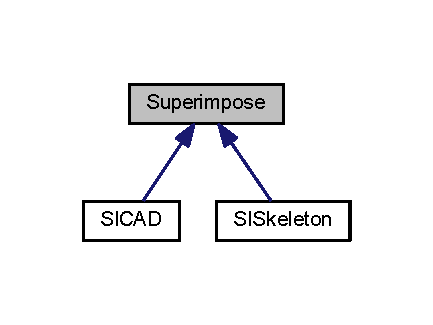
\includegraphics[width=208pt]{classSuperimpose__inherit__graph}
\end{center}
\end{figure}
\subsection*{Public Types}
\begin{DoxyCompactItemize}
\item 
typedef std\+::vector$<$ double $>$ \mbox{\hyperlink{classSuperimpose_a85d40a5caf19f486d1e0c15c0a025378}{Model\+Pose}}
\item 
typedef std\+::multimap$<$ std\+::string, \mbox{\hyperlink{classSuperimpose_a85d40a5caf19f486d1e0c15c0a025378}{Model\+Pose}} $>$ \mbox{\hyperlink{classSuperimpose_a178e3d4e2def6635bfcf9454dd4b5d22}{Model\+Pose\+Container}}
\item 
typedef std\+::pair$<$ std\+::string, \mbox{\hyperlink{classSuperimpose_a85d40a5caf19f486d1e0c15c0a025378}{Model\+Pose}} $>$ \mbox{\hyperlink{classSuperimpose_a1e02e0225687b42296dcfee4eadf8a55}{Model\+Pose\+Container\+Element}}
\end{DoxyCompactItemize}
\subsection*{Public Member Functions}
\begin{DoxyCompactItemize}
\item 
virtual \mbox{\hyperlink{classSuperimpose_a9e32031994dc105b1572e7a6db26b41b}{$\sim$\+Superimpose}} ()
\item 
virtual bool \mbox{\hyperlink{classSuperimpose_a62c4c269b8fc34cc36d3d54fa4acb35c}{superimpose}} (const \mbox{\hyperlink{classSuperimpose_a178e3d4e2def6635bfcf9454dd4b5d22}{Model\+Pose\+Container}} \&objpos\+\_\+map, const double $\ast$cam\+\_\+x, const double $\ast$cam\+\_\+o, cv\+::\+Mat \&img)=0
\end{DoxyCompactItemize}


\subsection{Detailed Description}


Definition at line 13 of file Superimpose.\+h.



\subsection{Member Typedef Documentation}
\mbox{\Hypertarget{classSuperimpose_a85d40a5caf19f486d1e0c15c0a025378}\label{classSuperimpose_a85d40a5caf19f486d1e0c15c0a025378}} 
\index{Superimpose@{Superimpose}!Model\+Pose@{Model\+Pose}}
\index{Model\+Pose@{Model\+Pose}!Superimpose@{Superimpose}}
\subsubsection{\texorpdfstring{Model\+Pose}{ModelPose}}
{\footnotesize\ttfamily typedef std\+::vector$<$double$>$ \mbox{\hyperlink{classSuperimpose_a85d40a5caf19f486d1e0c15c0a025378}{Superimpose\+::\+Model\+Pose}}}



Definition at line 16 of file Superimpose.\+h.

\mbox{\Hypertarget{classSuperimpose_a178e3d4e2def6635bfcf9454dd4b5d22}\label{classSuperimpose_a178e3d4e2def6635bfcf9454dd4b5d22}} 
\index{Superimpose@{Superimpose}!Model\+Pose\+Container@{Model\+Pose\+Container}}
\index{Model\+Pose\+Container@{Model\+Pose\+Container}!Superimpose@{Superimpose}}
\subsubsection{\texorpdfstring{Model\+Pose\+Container}{ModelPoseContainer}}
{\footnotesize\ttfamily typedef std\+::multimap$<$std\+::string, \mbox{\hyperlink{classSuperimpose_a85d40a5caf19f486d1e0c15c0a025378}{Model\+Pose}}$>$ \mbox{\hyperlink{classSuperimpose_a178e3d4e2def6635bfcf9454dd4b5d22}{Superimpose\+::\+Model\+Pose\+Container}}}



Definition at line 17 of file Superimpose.\+h.

\mbox{\Hypertarget{classSuperimpose_a1e02e0225687b42296dcfee4eadf8a55}\label{classSuperimpose_a1e02e0225687b42296dcfee4eadf8a55}} 
\index{Superimpose@{Superimpose}!Model\+Pose\+Container\+Element@{Model\+Pose\+Container\+Element}}
\index{Model\+Pose\+Container\+Element@{Model\+Pose\+Container\+Element}!Superimpose@{Superimpose}}
\subsubsection{\texorpdfstring{Model\+Pose\+Container\+Element}{ModelPoseContainerElement}}
{\footnotesize\ttfamily typedef std\+::pair$<$std\+::string, \mbox{\hyperlink{classSuperimpose_a85d40a5caf19f486d1e0c15c0a025378}{Model\+Pose}}$>$ \mbox{\hyperlink{classSuperimpose_a1e02e0225687b42296dcfee4eadf8a55}{Superimpose\+::\+Model\+Pose\+Container\+Element}}}



Definition at line 18 of file Superimpose.\+h.



\subsection{Constructor \& Destructor Documentation}
\mbox{\Hypertarget{classSuperimpose_a9e32031994dc105b1572e7a6db26b41b}\label{classSuperimpose_a9e32031994dc105b1572e7a6db26b41b}} 
\index{Superimpose@{Superimpose}!````~Superimpose@{$\sim$\+Superimpose}}
\index{````~Superimpose@{$\sim$\+Superimpose}!Superimpose@{Superimpose}}
\subsubsection{\texorpdfstring{$\sim$\+Superimpose()}{~Superimpose()}}
{\footnotesize\ttfamily virtual Superimpose\+::$\sim$\+Superimpose (\begin{DoxyParamCaption}{ }\end{DoxyParamCaption})\hspace{0.3cm}{\ttfamily [inline]}, {\ttfamily [virtual]}}



Definition at line 20 of file Superimpose.\+h.



\subsection{Member Function Documentation}
\mbox{\Hypertarget{classSuperimpose_a62c4c269b8fc34cc36d3d54fa4acb35c}\label{classSuperimpose_a62c4c269b8fc34cc36d3d54fa4acb35c}} 
\index{Superimpose@{Superimpose}!superimpose@{superimpose}}
\index{superimpose@{superimpose}!Superimpose@{Superimpose}}
\subsubsection{\texorpdfstring{superimpose()}{superimpose()}}
{\footnotesize\ttfamily virtual bool Superimpose\+::superimpose (\begin{DoxyParamCaption}\item[{const \mbox{\hyperlink{classSuperimpose_a178e3d4e2def6635bfcf9454dd4b5d22}{Model\+Pose\+Container}} \&}]{objpos\+\_\+map,  }\item[{const double $\ast$}]{cam\+\_\+x,  }\item[{const double $\ast$}]{cam\+\_\+o,  }\item[{cv\+::\+Mat \&}]{img }\end{DoxyParamCaption})\hspace{0.3cm}{\ttfamily [pure virtual]}}



Implemented in \mbox{\hyperlink{classSICAD_a356e0ac8a0f130952a72326bedd4ab60}{S\+I\+C\+AD}}, and \mbox{\hyperlink{classSISkeleton_a3f49fa3419370c2597435768f280c747}{S\+I\+Skeleton}}.



The documentation for this class was generated from the following file\+:\begin{DoxyCompactItemize}
\item 
C\+:/\+Users/cfantacci/\+Git\+Hub/superimpose-\/mesh-\/lib/src/\+Superimpose\+Mesh/include/\+Superimpose\+Mesh/\mbox{\hyperlink{Superimpose_8h}{Superimpose.\+h}}\end{DoxyCompactItemize}

\hypertarget{structTexture}{}\section{Texture Struct Reference}
\label{structTexture}\index{Texture@{Texture}}


{\ttfamily \#include $<$Mesh.\+h$>$}

\subsection*{Public Attributes}
\begin{DoxyCompactItemize}
\item 
G\+Luint \mbox{\hyperlink{structTexture_af848138d72c1fc995ab414a71ab10d47}{id}}
\item 
std\+::string \mbox{\hyperlink{structTexture_a916a835d009806f2a57546c7705942b1}{type}}
\item 
ai\+String \mbox{\hyperlink{structTexture_a88893bf81a4d4529c70da39f07f53ddb}{path}}
\end{DoxyCompactItemize}


\subsection{Detailed Description}


Definition at line 21 of file Mesh.\+h.



\subsection{Member Data Documentation}
\mbox{\Hypertarget{structTexture_af848138d72c1fc995ab414a71ab10d47}\label{structTexture_af848138d72c1fc995ab414a71ab10d47}} 
\index{Texture@{Texture}!id@{id}}
\index{id@{id}!Texture@{Texture}}
\subsubsection{\texorpdfstring{id}{id}}
{\footnotesize\ttfamily G\+Luint Texture\+::id}



Definition at line 22 of file Mesh.\+h.

\mbox{\Hypertarget{structTexture_a88893bf81a4d4529c70da39f07f53ddb}\label{structTexture_a88893bf81a4d4529c70da39f07f53ddb}} 
\index{Texture@{Texture}!path@{path}}
\index{path@{path}!Texture@{Texture}}
\subsubsection{\texorpdfstring{path}{path}}
{\footnotesize\ttfamily ai\+String Texture\+::path}



Definition at line 24 of file Mesh.\+h.

\mbox{\Hypertarget{structTexture_a916a835d009806f2a57546c7705942b1}\label{structTexture_a916a835d009806f2a57546c7705942b1}} 
\index{Texture@{Texture}!type@{type}}
\index{type@{type}!Texture@{Texture}}
\subsubsection{\texorpdfstring{type}{type}}
{\footnotesize\ttfamily std\+::string Texture\+::type}



Definition at line 23 of file Mesh.\+h.



The documentation for this struct was generated from the following file\+:\begin{DoxyCompactItemize}
\item 
C\+:/\+Users/cfantacci/\+Git\+Hub/superimpose-\/mesh-\/lib/src/\+Superimpose\+Mesh/include/\+Superimpose\+Mesh/\mbox{\hyperlink{Mesh_8h}{Mesh.\+h}}\end{DoxyCompactItemize}

\hypertarget{structVertex}{}\section{Vertex Struct Reference}
\label{structVertex}\index{Vertex@{Vertex}}


{\ttfamily \#include $<$Mesh.\+h$>$}

\subsection*{Public Attributes}
\begin{DoxyCompactItemize}
\item 
glm\+::vec3 \mbox{\hyperlink{structVertex_abb3cfacd96b5955b0cec9359840ee49f}{Position}}
\item 
glm\+::vec3 \mbox{\hyperlink{structVertex_a9ab4dc431b41509f0b1bb1a4bf09d4e2}{Normal}}
\item 
glm\+::vec2 \mbox{\hyperlink{structVertex_a921a513c1e6d1e63e99d477fa837a317}{Tex\+Coords}}
\end{DoxyCompactItemize}


\subsection{Detailed Description}


Definition at line 14 of file Mesh.\+h.



\subsection{Member Data Documentation}
\mbox{\Hypertarget{structVertex_a9ab4dc431b41509f0b1bb1a4bf09d4e2}\label{structVertex_a9ab4dc431b41509f0b1bb1a4bf09d4e2}} 
\index{Vertex@{Vertex}!Normal@{Normal}}
\index{Normal@{Normal}!Vertex@{Vertex}}
\subsubsection{\texorpdfstring{Normal}{Normal}}
{\footnotesize\ttfamily glm\+::vec3 Vertex\+::\+Normal}



Definition at line 16 of file Mesh.\+h.



Referenced by Model\+::process\+Mesh().

\mbox{\Hypertarget{structVertex_abb3cfacd96b5955b0cec9359840ee49f}\label{structVertex_abb3cfacd96b5955b0cec9359840ee49f}} 
\index{Vertex@{Vertex}!Position@{Position}}
\index{Position@{Position}!Vertex@{Vertex}}
\subsubsection{\texorpdfstring{Position}{Position}}
{\footnotesize\ttfamily glm\+::vec3 Vertex\+::\+Position}



Definition at line 15 of file Mesh.\+h.



Referenced by Model\+::process\+Mesh().

\mbox{\Hypertarget{structVertex_a921a513c1e6d1e63e99d477fa837a317}\label{structVertex_a921a513c1e6d1e63e99d477fa837a317}} 
\index{Vertex@{Vertex}!Tex\+Coords@{Tex\+Coords}}
\index{Tex\+Coords@{Tex\+Coords}!Vertex@{Vertex}}
\subsubsection{\texorpdfstring{Tex\+Coords}{TexCoords}}
{\footnotesize\ttfamily glm\+::vec2 Vertex\+::\+Tex\+Coords}



Definition at line 17 of file Mesh.\+h.



Referenced by Model\+::process\+Mesh().



The documentation for this struct was generated from the following file\+:\begin{DoxyCompactItemize}
\item 
C\+:/\+Users/cfantacci/\+Git\+Hub/superimpose-\/mesh-\/lib/src/\+Superimpose\+Mesh/include/\+Superimpose\+Mesh/\mbox{\hyperlink{Mesh_8h}{Mesh.\+h}}\end{DoxyCompactItemize}

\chapter{File Documentation}
\hypertarget{mainpage_8md}{}\section{mainpage.\+md File Reference}
\label{mainpage_8md}\index{mainpage.\+md@{mainpage.\+md}}

\hypertarget{tutorial__background_8cpp}{}\section{tutorial\+\_\+code/tutorial\+\_\+background.cpp File Reference}
\label{tutorial__background_8cpp}\index{tutorial\+\_\+code/tutorial\+\_\+background.\+cpp@{tutorial\+\_\+code/tutorial\+\_\+background.\+cpp}}
{\ttfamily \#include $<$cmath$>$}\newline
{\ttfamily \#include $<$exception$>$}\newline
{\ttfamily \#include $<$iostream$>$}\newline
{\ttfamily \#include $<$string$>$}\newline
{\ttfamily \#include $<$glm/glm.\+hpp$>$}\newline
{\ttfamily \#include $<$glm/gtc/matrix\+\_\+transform.\+hpp$>$}\newline
{\ttfamily \#include $<$opencv2/core/core.\+hpp$>$}\newline
{\ttfamily \#include $<$opencv2/imgcodecs/imgcodecs.\+hpp$>$}\newline
{\ttfamily \#include $<$opencv2/imgproc/imgproc.\+hpp$>$}\newline
{\ttfamily \#include $<$Superimpose\+Mesh/\+S\+I\+C\+A\+D.\+h$>$}\newline
Include dependency graph for tutorial\+\_\+background.\+cpp\+:
\nopagebreak
\begin{figure}[H]
\begin{center}
\leavevmode
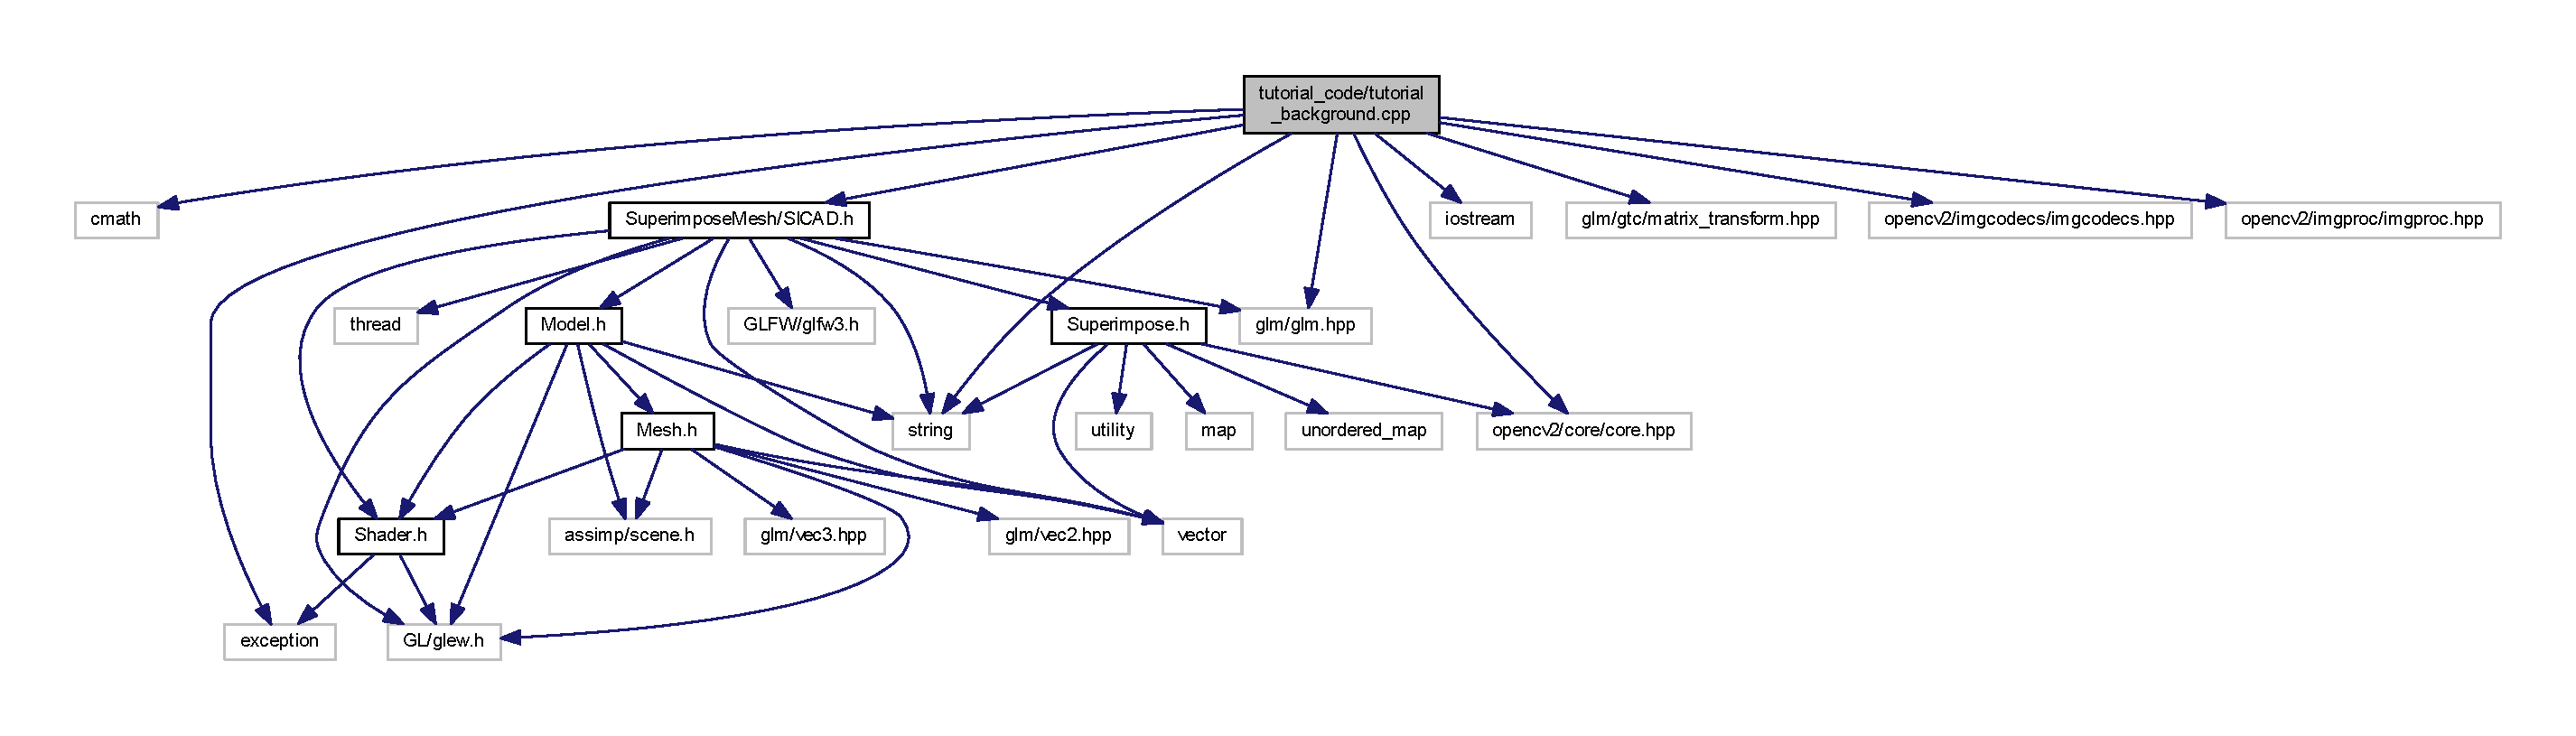
\includegraphics[width=350pt]{tutorial__background_8cpp__incl}
\end{center}
\end{figure}
\subsection*{Functions}
\begin{DoxyCompactItemize}
\item 
int \mbox{\hyperlink{tutorial__background_8cpp_ae66f6b31b5ad750f1fe042a706a4e3d4}{main}} ()
\end{DoxyCompactItemize}


\subsection{Function Documentation}
\mbox{\Hypertarget{tutorial__background_8cpp_ae66f6b31b5ad750f1fe042a706a4e3d4}\label{tutorial__background_8cpp_ae66f6b31b5ad750f1fe042a706a4e3d4}} 
\index{tutorial\+\_\+background.\+cpp@{tutorial\+\_\+background.\+cpp}!main@{main}}
\index{main@{main}!tutorial\+\_\+background.\+cpp@{tutorial\+\_\+background.\+cpp}}
\subsubsection{\texorpdfstring{main()}{main()}}
{\footnotesize\ttfamily int main (\begin{DoxyParamCaption}{ }\end{DoxyParamCaption})}



Definition at line 14 of file tutorial\+\_\+background.\+cpp.



References S\+I\+C\+A\+D\+::set\+Background\+Opt(), and S\+I\+C\+A\+D\+::superimpose().

Here is the call graph for this function\+:
\nopagebreak
\begin{figure}[H]
\begin{center}
\leavevmode
\includegraphics[width=350pt]{tutorial__background_8cpp_ae66f6b31b5ad750f1fe042a706a4e3d4_cgraph}
\end{center}
\end{figure}

\hypertarget{tutorial__superimpose_8cpp}{}\section{tutorial\+\_\+code/tutorial\+\_\+superimpose.cpp File Reference}
\label{tutorial__superimpose_8cpp}\index{tutorial\+\_\+code/tutorial\+\_\+superimpose.\+cpp@{tutorial\+\_\+code/tutorial\+\_\+superimpose.\+cpp}}
{\ttfamily \#include $<$cmath$>$}\newline
{\ttfamily \#include $<$exception$>$}\newline
{\ttfamily \#include $<$iostream$>$}\newline
{\ttfamily \#include $<$string$>$}\newline
{\ttfamily \#include $<$glm/glm.\+hpp$>$}\newline
{\ttfamily \#include $<$glm/gtc/matrix\+\_\+transform.\+hpp$>$}\newline
{\ttfamily \#include $<$opencv2/core/core.\+hpp$>$}\newline
{\ttfamily \#include $<$opencv2/imgcodecs/imgcodecs.\+hpp$>$}\newline
{\ttfamily \#include $<$opencv2/imgproc/imgproc.\+hpp$>$}\newline
{\ttfamily \#include $<$Superimpose\+Mesh/\+S\+I\+C\+A\+D.\+h$>$}\newline
Include dependency graph for tutorial\+\_\+superimpose.\+cpp\+:
\nopagebreak
\begin{figure}[H]
\begin{center}
\leavevmode
\includegraphics[width=350pt]{tutorial__superimpose_8cpp__incl}
\end{center}
\end{figure}
\subsection*{Functions}
\begin{DoxyCompactItemize}
\item 
int \mbox{\hyperlink{tutorial__superimpose_8cpp_ae66f6b31b5ad750f1fe042a706a4e3d4}{main}} ()
\end{DoxyCompactItemize}


\subsection{Function Documentation}
\mbox{\Hypertarget{tutorial__superimpose_8cpp_ae66f6b31b5ad750f1fe042a706a4e3d4}\label{tutorial__superimpose_8cpp_ae66f6b31b5ad750f1fe042a706a4e3d4}} 
\index{tutorial\+\_\+superimpose.\+cpp@{tutorial\+\_\+superimpose.\+cpp}!main@{main}}
\index{main@{main}!tutorial\+\_\+superimpose.\+cpp@{tutorial\+\_\+superimpose.\+cpp}}
\subsubsection{\texorpdfstring{main()}{main()}}
{\footnotesize\ttfamily int main (\begin{DoxyParamCaption}{ }\end{DoxyParamCaption})}



Definition at line 14 of file tutorial\+\_\+superimpose.\+cpp.



References S\+I\+C\+A\+D\+::superimpose().

Here is the call graph for this function\+:
\nopagebreak
\begin{figure}[H]
\begin{center}
\leavevmode
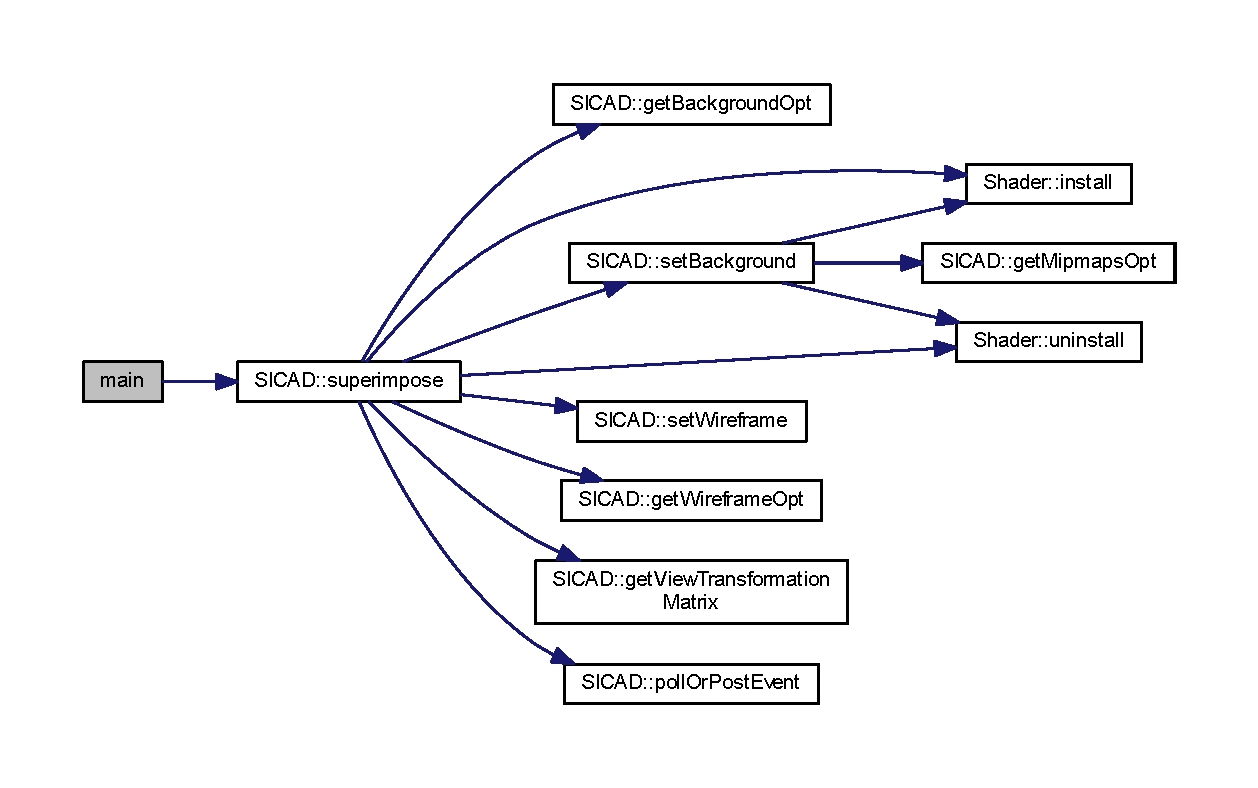
\includegraphics[width=350pt]{tutorial__superimpose_8cpp_ae66f6b31b5ad750f1fe042a706a4e3d4_cgraph}
\end{center}
\end{figure}

\hypertarget{tutorial__superimpose_8md}{}\section{tutorial\+\_\+superimpose.\+md File Reference}
\label{tutorial__superimpose_8md}\index{tutorial\+\_\+superimpose.\+md@{tutorial\+\_\+superimpose.\+md}}

\hypertarget{tutorial__superimpose__background_8md}{}\section{tutorial\+\_\+superimpose\+\_\+background.\+md File Reference}
\label{tutorial__superimpose__background_8md}\index{tutorial\+\_\+superimpose\+\_\+background.\+md@{tutorial\+\_\+superimpose\+\_\+background.\+md}}

\hypertarget{Mesh_8h}{}\section{C\+:/\+Users/cfantacci/\+Git\+Hub/superimpose-\/mesh-\/lib/src/\+Superimpose\+Mesh/include/\+Superimpose\+Mesh/\+Mesh.h File Reference}
\label{Mesh_8h}\index{C\+:/\+Users/cfantacci/\+Git\+Hub/superimpose-\/mesh-\/lib/src/\+Superimpose\+Mesh/include/\+Superimpose\+Mesh/\+Mesh.\+h@{C\+:/\+Users/cfantacci/\+Git\+Hub/superimpose-\/mesh-\/lib/src/\+Superimpose\+Mesh/include/\+Superimpose\+Mesh/\+Mesh.\+h}}
{\ttfamily \#include \char`\"{}Shader.\+h\char`\"{}}\newline
{\ttfamily \#include $<$vector$>$}\newline
{\ttfamily \#include $<$G\+L/glew.\+h$>$}\newline
{\ttfamily \#include $<$glm/vec2.\+hpp$>$}\newline
{\ttfamily \#include $<$glm/vec3.\+hpp$>$}\newline
{\ttfamily \#include $<$assimp/scene.\+h$>$}\newline
Include dependency graph for Mesh.\+h\+:
\nopagebreak
\begin{figure}[H]
\begin{center}
\leavevmode
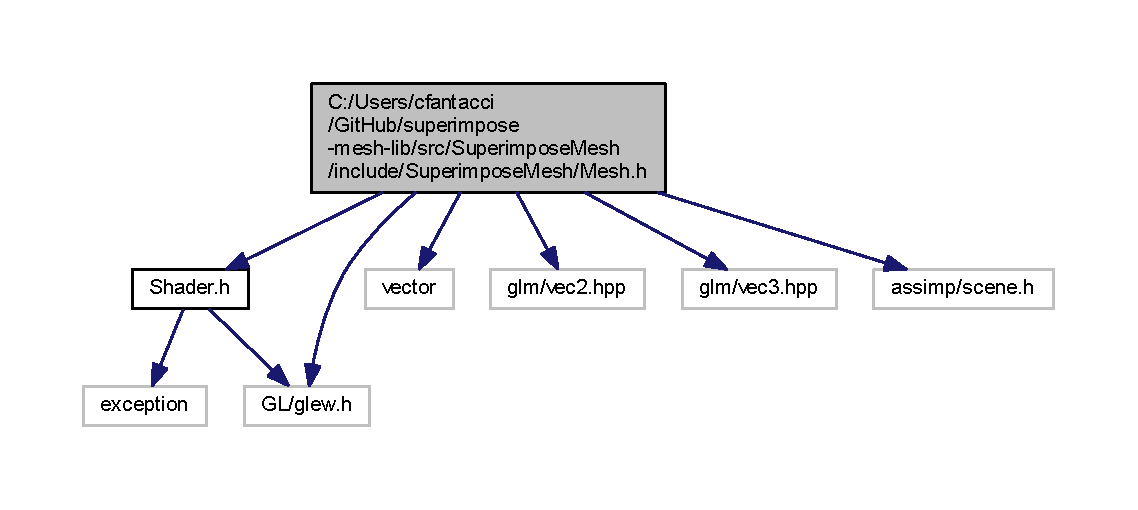
\includegraphics[width=350pt]{Mesh_8h__incl}
\end{center}
\end{figure}
This graph shows which files directly or indirectly include this file\+:
\nopagebreak
\begin{figure}[H]
\begin{center}
\leavevmode
\includegraphics[width=350pt]{Mesh_8h__dep__incl}
\end{center}
\end{figure}
\subsection*{Classes}
\begin{DoxyCompactItemize}
\item 
struct \mbox{\hyperlink{structVertex}{Vertex}}
\item 
struct \mbox{\hyperlink{structTexture}{Texture}}
\item 
class \mbox{\hyperlink{classMesh}{Mesh}}
\end{DoxyCompactItemize}

\hypertarget{Model_8h}{}\section{C\+:/\+Users/cfantacci/\+Git\+Hub/superimpose-\/mesh-\/lib/src/\+Superimpose\+Mesh/include/\+Superimpose\+Mesh/\+Model.h File Reference}
\label{Model_8h}\index{C\+:/\+Users/cfantacci/\+Git\+Hub/superimpose-\/mesh-\/lib/src/\+Superimpose\+Mesh/include/\+Superimpose\+Mesh/\+Model.\+h@{C\+:/\+Users/cfantacci/\+Git\+Hub/superimpose-\/mesh-\/lib/src/\+Superimpose\+Mesh/include/\+Superimpose\+Mesh/\+Model.\+h}}
{\ttfamily \#include \char`\"{}Shader.\+h\char`\"{}}\newline
{\ttfamily \#include \char`\"{}Mesh.\+h\char`\"{}}\newline
{\ttfamily \#include $<$vector$>$}\newline
{\ttfamily \#include $<$string$>$}\newline
{\ttfamily \#include $<$G\+L/glew.\+h$>$}\newline
{\ttfamily \#include $<$assimp/scene.\+h$>$}\newline
Include dependency graph for Model.\+h\+:
\nopagebreak
\begin{figure}[H]
\begin{center}
\leavevmode
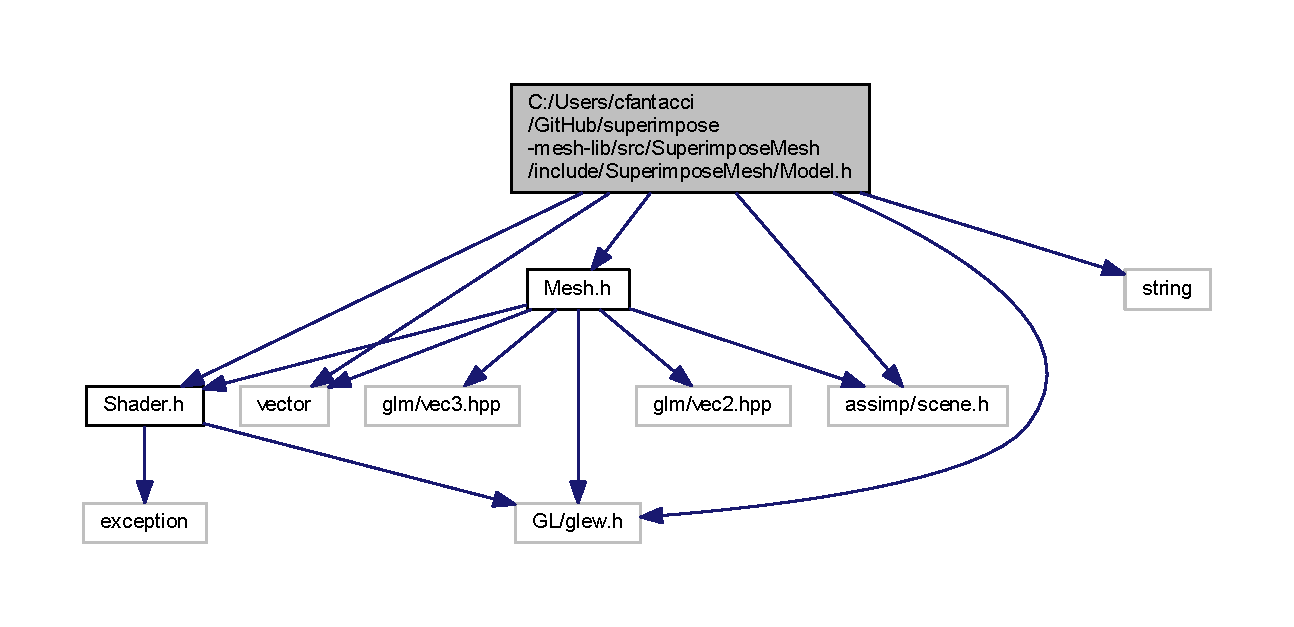
\includegraphics[width=350pt]{Model_8h__incl}
\end{center}
\end{figure}
This graph shows which files directly or indirectly include this file\+:
\nopagebreak
\begin{figure}[H]
\begin{center}
\leavevmode
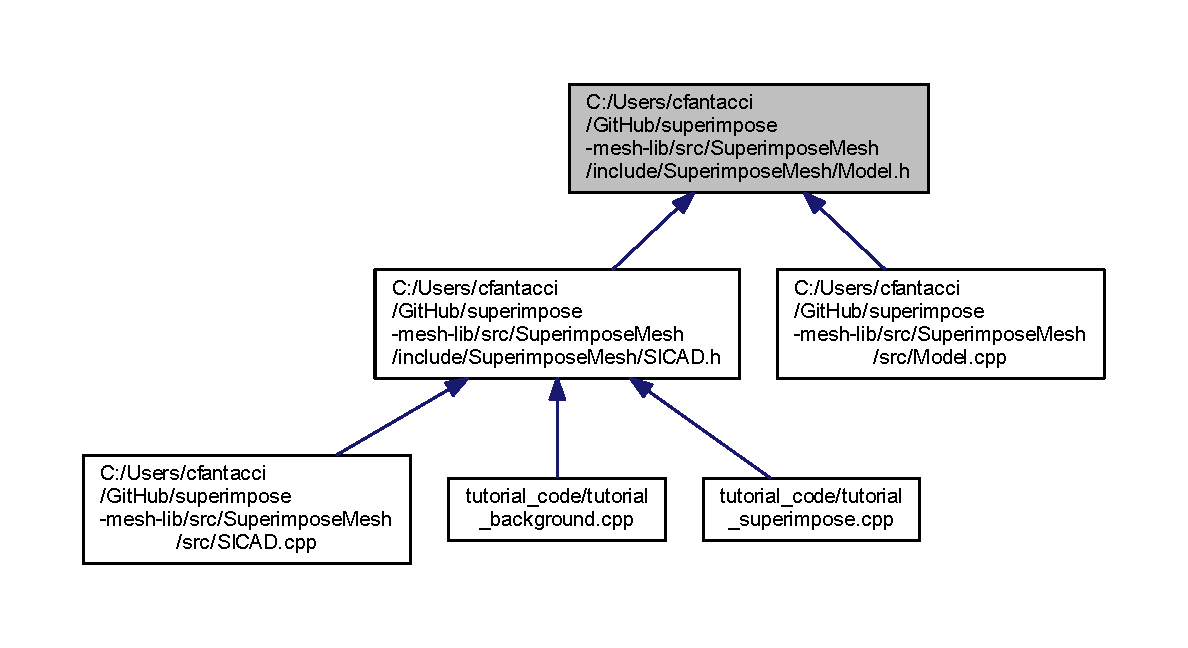
\includegraphics[width=350pt]{Model_8h__dep__incl}
\end{center}
\end{figure}
\subsection*{Classes}
\begin{DoxyCompactItemize}
\item 
class \mbox{\hyperlink{classModel}{Model}}
\end{DoxyCompactItemize}

\hypertarget{Shader_8h}{}\section{C\+:/\+Users/cfantacci/\+Git\+Hub/superimpose-\/mesh-\/lib/src/\+Superimpose\+Mesh/include/\+Superimpose\+Mesh/\+Shader.h File Reference}
\label{Shader_8h}\index{C\+:/\+Users/cfantacci/\+Git\+Hub/superimpose-\/mesh-\/lib/src/\+Superimpose\+Mesh/include/\+Superimpose\+Mesh/\+Shader.\+h@{C\+:/\+Users/cfantacci/\+Git\+Hub/superimpose-\/mesh-\/lib/src/\+Superimpose\+Mesh/include/\+Superimpose\+Mesh/\+Shader.\+h}}
{\ttfamily \#include $<$exception$>$}\newline
{\ttfamily \#include $<$G\+L/glew.\+h$>$}\newline
Include dependency graph for Shader.\+h\+:
\nopagebreak
\begin{figure}[H]
\begin{center}
\leavevmode
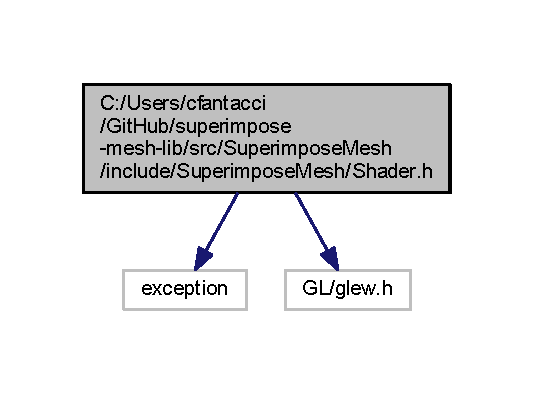
\includegraphics[width=256pt]{Shader_8h__incl}
\end{center}
\end{figure}
This graph shows which files directly or indirectly include this file\+:
\nopagebreak
\begin{figure}[H]
\begin{center}
\leavevmode
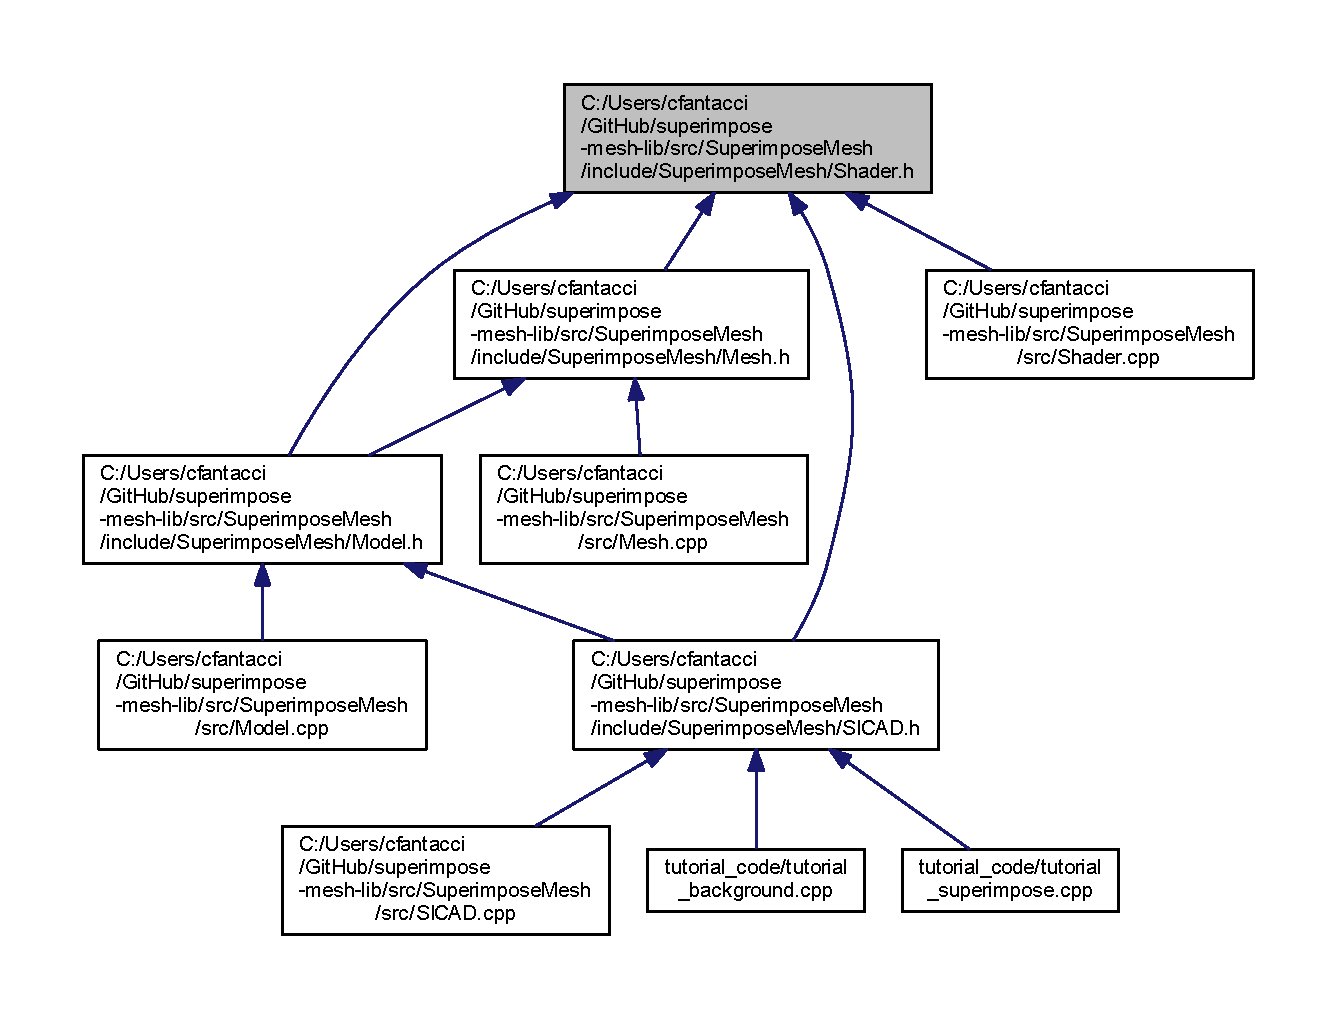
\includegraphics[width=350pt]{Shader_8h__dep__incl}
\end{center}
\end{figure}
\subsection*{Classes}
\begin{DoxyCompactItemize}
\item 
class \mbox{\hyperlink{classShader}{Shader}}
\end{DoxyCompactItemize}

\hypertarget{SICAD_8h}{}\section{C\+:/\+Users/cfantacci/\+Git\+Hub/superimpose-\/mesh-\/lib/src/\+Superimpose\+Mesh/include/\+Superimpose\+Mesh/\+S\+I\+C\+AD.h File Reference}
\label{SICAD_8h}\index{C\+:/\+Users/cfantacci/\+Git\+Hub/superimpose-\/mesh-\/lib/src/\+Superimpose\+Mesh/include/\+Superimpose\+Mesh/\+S\+I\+C\+A\+D.\+h@{C\+:/\+Users/cfantacci/\+Git\+Hub/superimpose-\/mesh-\/lib/src/\+Superimpose\+Mesh/include/\+Superimpose\+Mesh/\+S\+I\+C\+A\+D.\+h}}
{\ttfamily \#include \char`\"{}Superimpose.\+h\char`\"{}}\newline
{\ttfamily \#include \char`\"{}Model.\+h\char`\"{}}\newline
{\ttfamily \#include \char`\"{}Shader.\+h\char`\"{}}\newline
{\ttfamily \#include $<$string$>$}\newline
{\ttfamily \#include $<$thread$>$}\newline
{\ttfamily \#include $<$vector$>$}\newline
{\ttfamily \#include $<$G\+L/glew.\+h$>$}\newline
{\ttfamily \#include $<$G\+L\+F\+W/glfw3.\+h$>$}\newline
{\ttfamily \#include $<$glm/glm.\+hpp$>$}\newline
Include dependency graph for S\+I\+C\+A\+D.\+h\+:
\nopagebreak
\begin{figure}[H]
\begin{center}
\leavevmode
\includegraphics[width=350pt]{SICAD_8h__incl}
\end{center}
\end{figure}
This graph shows which files directly or indirectly include this file\+:
\nopagebreak
\begin{figure}[H]
\begin{center}
\leavevmode
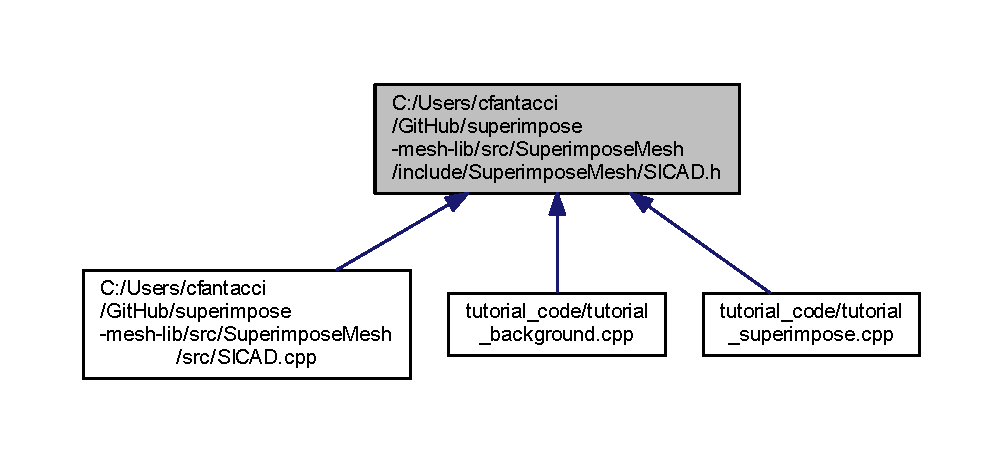
\includegraphics[width=350pt]{SICAD_8h__dep__incl}
\end{center}
\end{figure}
\subsection*{Classes}
\begin{DoxyCompactItemize}
\item 
class \mbox{\hyperlink{classSICAD}{S\+I\+C\+AD}}
\begin{DoxyCompactList}\small\item\em A \mbox{\hyperlink{classSuperimpose}{Superimpose}} derived class to superimpose mesh models on top of images. \end{DoxyCompactList}\end{DoxyCompactItemize}

\hypertarget{SISkeleton_8h}{}\section{C\+:/\+Users/cfantacci/\+Git\+Hub/superimpose-\/mesh-\/lib/src/\+Superimpose\+Mesh/include/\+Superimpose\+Mesh/\+S\+I\+Skeleton.h File Reference}
\label{SISkeleton_8h}\index{C\+:/\+Users/cfantacci/\+Git\+Hub/superimpose-\/mesh-\/lib/src/\+Superimpose\+Mesh/include/\+Superimpose\+Mesh/\+S\+I\+Skeleton.\+h@{C\+:/\+Users/cfantacci/\+Git\+Hub/superimpose-\/mesh-\/lib/src/\+Superimpose\+Mesh/include/\+Superimpose\+Mesh/\+S\+I\+Skeleton.\+h}}
{\ttfamily \#include \char`\"{}Superimpose.\+h\char`\"{}}\newline
{\ttfamily \#include $<$list$>$}\newline
{\ttfamily \#include $<$string$>$}\newline
{\ttfamily \#include $<$glm/glm.\+hpp$>$}\newline
Include dependency graph for S\+I\+Skeleton.\+h\+:
\nopagebreak
\begin{figure}[H]
\begin{center}
\leavevmode
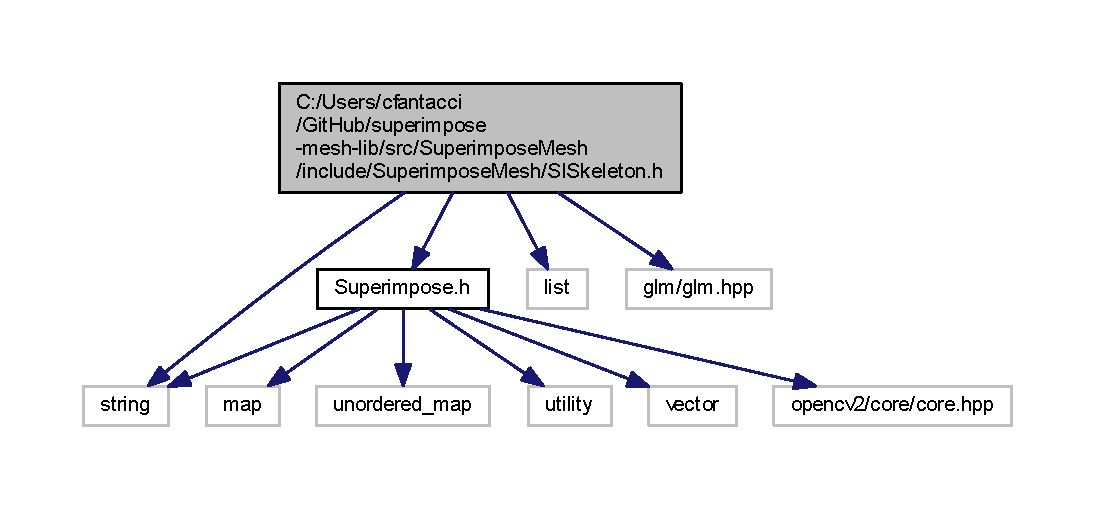
\includegraphics[width=350pt]{SISkeleton_8h__incl}
\end{center}
\end{figure}
This graph shows which files directly or indirectly include this file\+:
\nopagebreak
\begin{figure}[H]
\begin{center}
\leavevmode
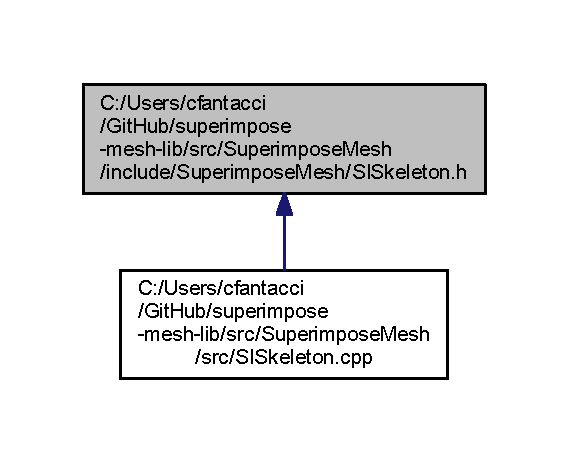
\includegraphics[width=273pt]{SISkeleton_8h__dep__incl}
\end{center}
\end{figure}
\subsection*{Classes}
\begin{DoxyCompactItemize}
\item 
class \mbox{\hyperlink{classSISkeleton}{S\+I\+Skeleton}}
\end{DoxyCompactItemize}

\hypertarget{Superimpose_8h}{}\section{C\+:/\+Users/cfantacci/\+Git\+Hub/superimpose-\/mesh-\/lib/src/\+Superimpose\+Mesh/include/\+Superimpose\+Mesh/\+Superimpose.h File Reference}
\label{Superimpose_8h}\index{C\+:/\+Users/cfantacci/\+Git\+Hub/superimpose-\/mesh-\/lib/src/\+Superimpose\+Mesh/include/\+Superimpose\+Mesh/\+Superimpose.\+h@{C\+:/\+Users/cfantacci/\+Git\+Hub/superimpose-\/mesh-\/lib/src/\+Superimpose\+Mesh/include/\+Superimpose\+Mesh/\+Superimpose.\+h}}
{\ttfamily \#include $<$string$>$}\newline
{\ttfamily \#include $<$map$>$}\newline
{\ttfamily \#include $<$unordered\+\_\+map$>$}\newline
{\ttfamily \#include $<$utility$>$}\newline
{\ttfamily \#include $<$vector$>$}\newline
{\ttfamily \#include $<$opencv2/core/core.\+hpp$>$}\newline
Include dependency graph for Superimpose.\+h\+:
\nopagebreak
\begin{figure}[H]
\begin{center}
\leavevmode
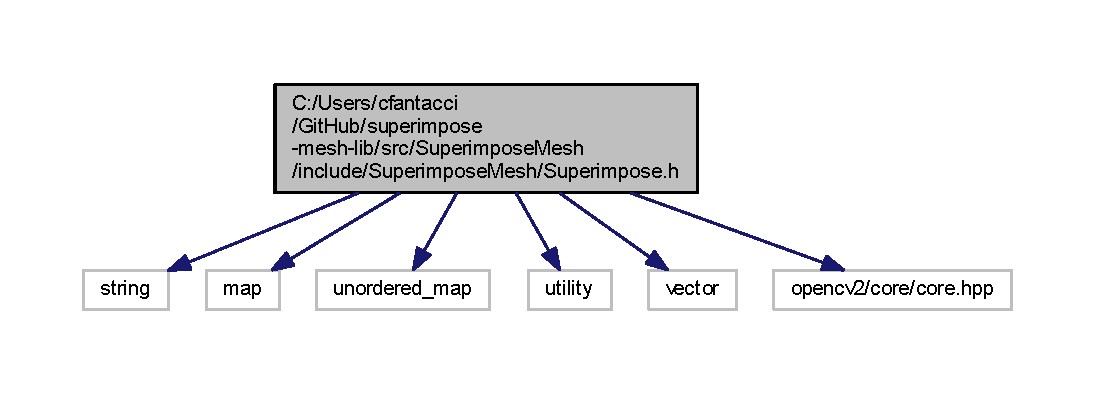
\includegraphics[width=350pt]{Superimpose_8h__incl}
\end{center}
\end{figure}
This graph shows which files directly or indirectly include this file\+:
\nopagebreak
\begin{figure}[H]
\begin{center}
\leavevmode
\includegraphics[width=350pt]{Superimpose_8h__dep__incl}
\end{center}
\end{figure}
\subsection*{Classes}
\begin{DoxyCompactItemize}
\item 
class \mbox{\hyperlink{classSuperimpose}{Superimpose}}
\end{DoxyCompactItemize}

\hypertarget{Mesh_8cpp}{}\section{C\+:/\+Users/cfantacci/\+Git\+Hub/superimpose-\/mesh-\/lib/src/\+Superimpose\+Mesh/src/\+Mesh.cpp File Reference}
\label{Mesh_8cpp}\index{C\+:/\+Users/cfantacci/\+Git\+Hub/superimpose-\/mesh-\/lib/src/\+Superimpose\+Mesh/src/\+Mesh.\+cpp@{C\+:/\+Users/cfantacci/\+Git\+Hub/superimpose-\/mesh-\/lib/src/\+Superimpose\+Mesh/src/\+Mesh.\+cpp}}
{\ttfamily \#include \char`\"{}Superimpose\+Mesh/\+Mesh.\+h\char`\"{}}\newline
{\ttfamily \#include $<$string$>$}\newline
{\ttfamily \#include $<$glm/glm.\+hpp$>$}\newline
{\ttfamily \#include $<$glm/gtc/matrix\+\_\+transform.\+hpp$>$}\newline
{\ttfamily \#include $<$glm/gtc/type\+\_\+ptr.\+hpp$>$}\newline
Include dependency graph for Mesh.\+cpp\+:
\nopagebreak
\begin{figure}[H]
\begin{center}
\leavevmode
\includegraphics[width=350pt]{Mesh_8cpp__incl}
\end{center}
\end{figure}

\hypertarget{Model_8cpp}{}\section{C\+:/\+Users/cfantacci/\+Git\+Hub/superimpose-\/mesh-\/lib/src/\+Superimpose\+Mesh/src/\+Model.cpp File Reference}
\label{Model_8cpp}\index{C\+:/\+Users/cfantacci/\+Git\+Hub/superimpose-\/mesh-\/lib/src/\+Superimpose\+Mesh/src/\+Model.\+cpp@{C\+:/\+Users/cfantacci/\+Git\+Hub/superimpose-\/mesh-\/lib/src/\+Superimpose\+Mesh/src/\+Model.\+cpp}}
{\ttfamily \#include \char`\"{}Superimpose\+Mesh/\+Model.\+h\char`\"{}}\newline
{\ttfamily \#include $<$iostream$>$}\newline
{\ttfamily \#include $<$assimp/\+Importer.\+hpp$>$}\newline
{\ttfamily \#include $<$assimp/postprocess.\+h$>$}\newline
{\ttfamily \#include $<$glm/glm.\+hpp$>$}\newline
Include dependency graph for Model.\+cpp\+:
\nopagebreak
\begin{figure}[H]
\begin{center}
\leavevmode
\includegraphics[width=350pt]{Model_8cpp__incl}
\end{center}
\end{figure}

\hypertarget{Shader_8cpp}{}\section{C\+:/\+Users/cfantacci/\+Git\+Hub/superimpose-\/mesh-\/lib/src/\+Superimpose\+Mesh/src/\+Shader.cpp File Reference}
\label{Shader_8cpp}\index{C\+:/\+Users/cfantacci/\+Git\+Hub/superimpose-\/mesh-\/lib/src/\+Superimpose\+Mesh/src/\+Shader.\+cpp@{C\+:/\+Users/cfantacci/\+Git\+Hub/superimpose-\/mesh-\/lib/src/\+Superimpose\+Mesh/src/\+Shader.\+cpp}}
{\ttfamily \#include \char`\"{}Superimpose\+Mesh/\+Shader.\+h\char`\"{}}\newline
{\ttfamily \#include $<$string$>$}\newline
{\ttfamily \#include $<$fstream$>$}\newline
{\ttfamily \#include $<$sstream$>$}\newline
{\ttfamily \#include $<$iostream$>$}\newline
Include dependency graph for Shader.\+cpp\+:
\nopagebreak
\begin{figure}[H]
\begin{center}
\leavevmode
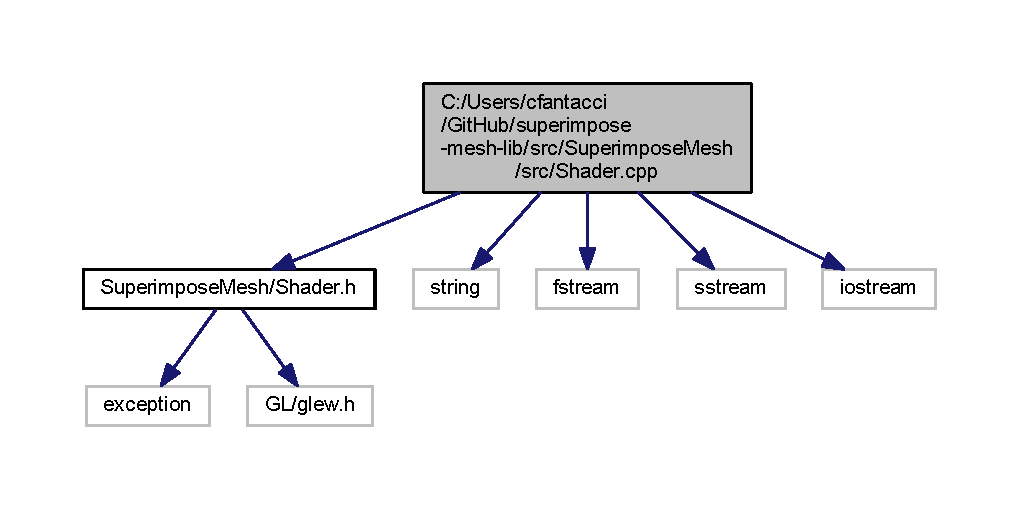
\includegraphics[width=350pt]{Shader_8cpp__incl}
\end{center}
\end{figure}

\hypertarget{SICAD_8cpp}{}\section{C\+:/\+Users/cfantacci/\+Git\+Hub/superimpose-\/mesh-\/lib/src/\+Superimpose\+Mesh/src/\+S\+I\+C\+AD.cpp File Reference}
\label{SICAD_8cpp}\index{C\+:/\+Users/cfantacci/\+Git\+Hub/superimpose-\/mesh-\/lib/src/\+Superimpose\+Mesh/src/\+S\+I\+C\+A\+D.\+cpp@{C\+:/\+Users/cfantacci/\+Git\+Hub/superimpose-\/mesh-\/lib/src/\+Superimpose\+Mesh/src/\+S\+I\+C\+A\+D.\+cpp}}
{\ttfamily \#include \char`\"{}Superimpose\+Mesh/\+S\+I\+C\+A\+D.\+h\char`\"{}}\newline
{\ttfamily \#include $<$iostream$>$}\newline
{\ttfamily \#include $<$exception$>$}\newline
{\ttfamily \#include $<$string$>$}\newline
{\ttfamily \#include $<$assimp/\+Importer.\+hpp$>$}\newline
{\ttfamily \#include $<$assimp/scene.\+h$>$}\newline
{\ttfamily \#include $<$assimp/postprocess.\+h$>$}\newline
{\ttfamily \#include $<$glm/gtc/matrix\+\_\+transform.\+hpp$>$}\newline
{\ttfamily \#include $<$glm/gtc/type\+\_\+ptr.\+hpp$>$}\newline
{\ttfamily \#include $<$opencv2/imgproc/imgproc.\+hpp$>$}\newline
Include dependency graph for S\+I\+C\+A\+D.\+cpp\+:
\nopagebreak
\begin{figure}[H]
\begin{center}
\leavevmode
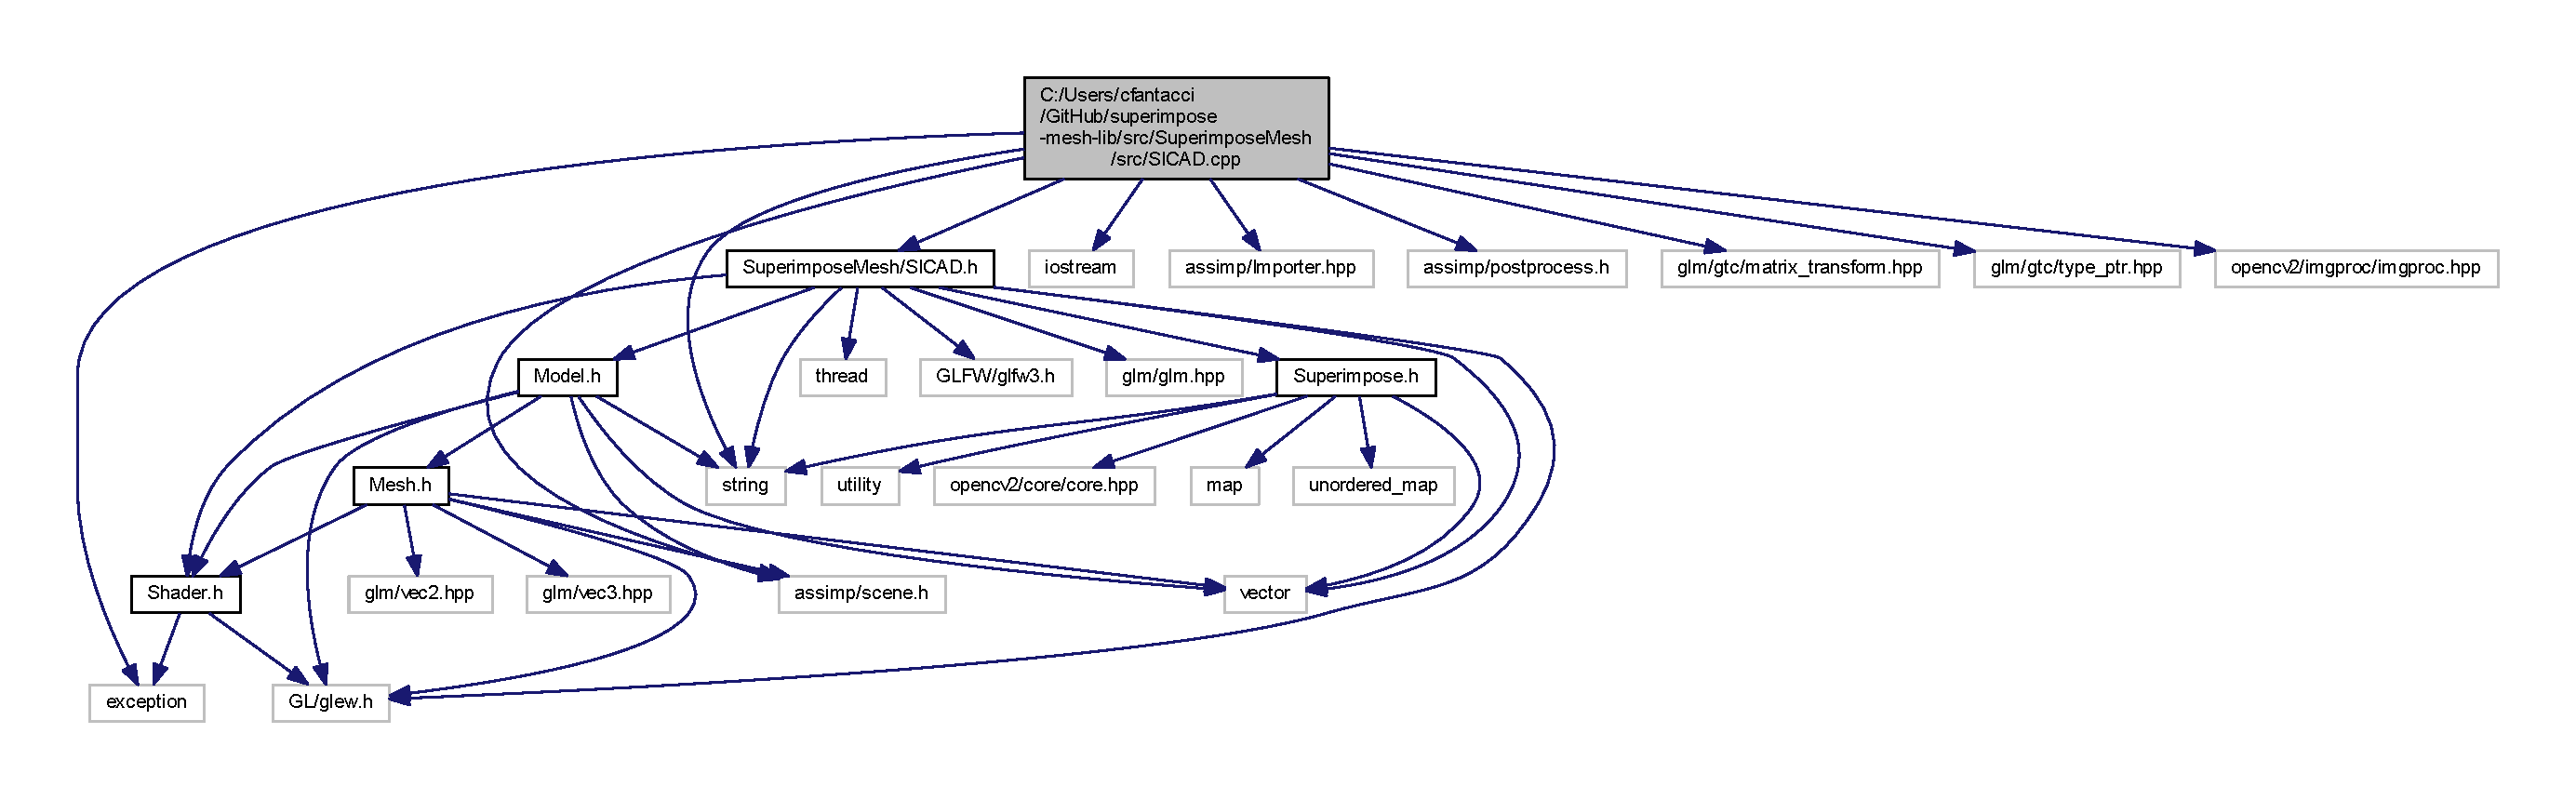
\includegraphics[width=350pt]{SICAD_8cpp__incl}
\end{center}
\end{figure}

\hypertarget{SISkeleton_8cpp}{}\section{C\+:/\+Users/cfantacci/\+Git\+Hub/superimpose-\/mesh-\/lib/src/\+Superimpose\+Mesh/src/\+S\+I\+Skeleton.cpp File Reference}
\label{SISkeleton_8cpp}\index{C\+:/\+Users/cfantacci/\+Git\+Hub/superimpose-\/mesh-\/lib/src/\+Superimpose\+Mesh/src/\+S\+I\+Skeleton.\+cpp@{C\+:/\+Users/cfantacci/\+Git\+Hub/superimpose-\/mesh-\/lib/src/\+Superimpose\+Mesh/src/\+S\+I\+Skeleton.\+cpp}}
{\ttfamily \#include \char`\"{}Superimpose\+Mesh/\+S\+I\+Skeleton.\+h\char`\"{}}\newline
{\ttfamily \#include $<$iostream$>$}\newline
{\ttfamily \#include $<$glm/gtc/matrix\+\_\+transform.\+hpp$>$}\newline
{\ttfamily \#include $<$glm/gtc/type\+\_\+ptr.\+hpp$>$}\newline
{\ttfamily \#include $<$opencv2/core/core.\+hpp$>$}\newline
{\ttfamily \#include $<$opencv2/imgproc/imgproc.\+hpp$>$}\newline
{\ttfamily \#include $<$opencv2/calib3d/calib3d.\+hpp$>$}\newline
Include dependency graph for S\+I\+Skeleton.\+cpp\+:
\nopagebreak
\begin{figure}[H]
\begin{center}
\leavevmode
\includegraphics[width=350pt]{SISkeleton_8cpp__incl}
\end{center}
\end{figure}

%--- End generated contents ---

% Index
\backmatter
\newpage
\phantomsection
\clearemptydoublepage
\addcontentsline{toc}{chapter}{Index}
\printindex

\end{document}
